\chapter{Results and Discussion}
\label{ch:ResultsDiscussion}

The preceding chapters defined a rigorous simulation framework and parameter sweep for both flow-optimised and eco-driving \ac{glosa} controllers. We now explore how these algorithms perform under varying traffic loads and penetration rates, revealing their network-level and vehicle-level impacts.  
We open with an analysis of green‐phase vehicle flow to understand discharge performance under connected control (\ref{sec:Results_GreenPhaseFlow}). From there, attention moves to vehicle dynamics: first average travel speed (\ref{sec:Results_MeanSpeed}), then stop frequency (\ref{sec:Results_Stops}), and finally driving smoothness via acceleration profiles (\ref{sec:Results_Smoothness}). Environmental consequences follow, as per-vehicle CO$_2$ and NO$_x$ emissions, quantify ecological benefit (\ref{sec:Results_Emissions}). A dedicated break-even analysis then pinpoints the critical penetration at which eco-driving gains outweigh flow-optimised advantages (\ref{sec:Results_BreakEven}). Computational viability comes next, comparing runtime overheads of the advisory loop and optimisation algorithm (\ref{sec:Results_Computational}). We conclude by synthesising these findings, discussing trade-offs and implications for real-world deployment (\ref{sec:Results_Discussion}).  

\section{Green‐Phase Vehicle Flow}
\label{sec:Results_GreenPhaseFlow}

The per-cycle vehicle flow for demand levels ranging from $69$ to $3462~\unit{\veh\per\hour}$ across \acp{mpr} is summarized in Table~\vref{tab:GreenPhaseFlow}. Where \enquote{Standard} (0\%) denotes no \ac{glosa}, and \enquote{Baseline} denotes \ac{flow-glosa}. Figures~\vref{fig:HBEFA4_Flow} and \vref{fig:PHEM_Flow} visualise these curves for HBEFA4 and PHEMlight5 at $1500$, $2000$ and $2500~\unit{\veh\per\hour}$. 
At low to moderate demand ($69$--$692~\unit{\veh\per\hour}$) both \ac{eco-glosa} and \ac{flow-glosa} remain within $\pm 0.1$ vehicles of the Standard across the full \ac{mpr} range, indicating that under light traffic densities speed advisories, whether emission‐ or flow‐optimised, do not materially affect green‐phase capacity. As demand rises to $1385~\unit{\veh\per\hour}$, a slight scatter appears in the \ac{eco-glosa} curve at low \ac{mpr} ($10$--$30\%$), yet maximum deviation stays under $0.13$ vehicles, still within normal cycle‐to‐cycle variation. Crucially, this insensitivity of \ac{eco-glosa} extends only up to $2077~\unit{\veh\per\hour}$ for PHEMlight5 and up to $2769~\unit{\veh\per\hour}$ for HBEFA4, suggesting that the coarser emission factors in HBEFA4 delay the onset of aggressive speed changes. Beyond these breakpoints, the throughput of the \ac{eco-glosa} controller declines sharply. For instance, at a demand of $2769~\unit{\veh\per\hour}$ under the PHEMlight5 model, the flow drops from $46.03$ vehicles at Standard to $35.9$ vehicles at $90\%$ \ac{mpr}, a reduction of $22\%$. A similar decline occurs at $3462~\unit{\veh\per\hour}$ with the HBEFA4 model, where throughput falls from $49.03$ to $37.27$ vehicles at full \ac{mpr}. This provides clear evidence of queue formation and spill-back occurring within a single green phase. In contrast, the \ac{flow-glosa} baseline curves remain essentially horizontal across all volumes and \ac{mpr}s, preserving 100\% of Standard throughput by design. These results confirm that while \ac{eco-glosa} can marginally modulate flow under low densities, its emission‐driven advisories incur significant capacity penalties under high demand, whereas \ac{flow-glosa} reliably maintains green‐phase capacity in all tested scenarios.
\begin{figure}[htb]
  \centering
  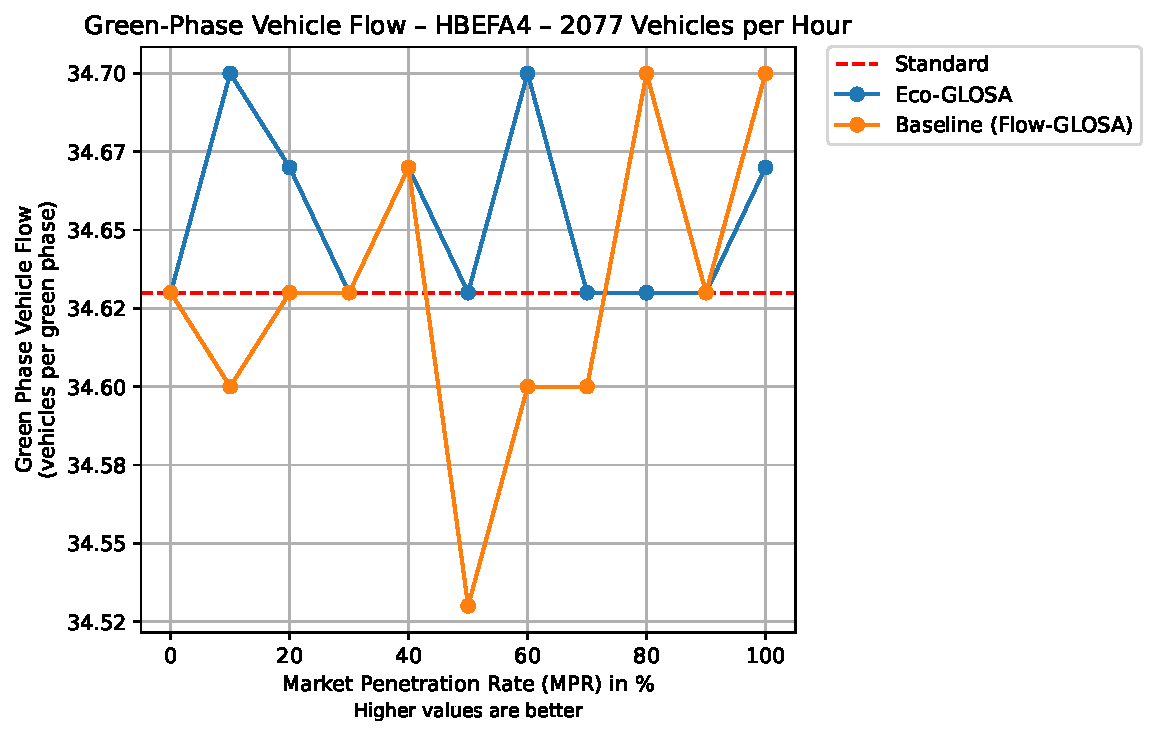
\includegraphics[width=0.49\textwidth]{data/img/GreenPhaseVehicleFlow/GreenPhaseVehicleFlow_HBEFA4_Cars1500.pdf}
  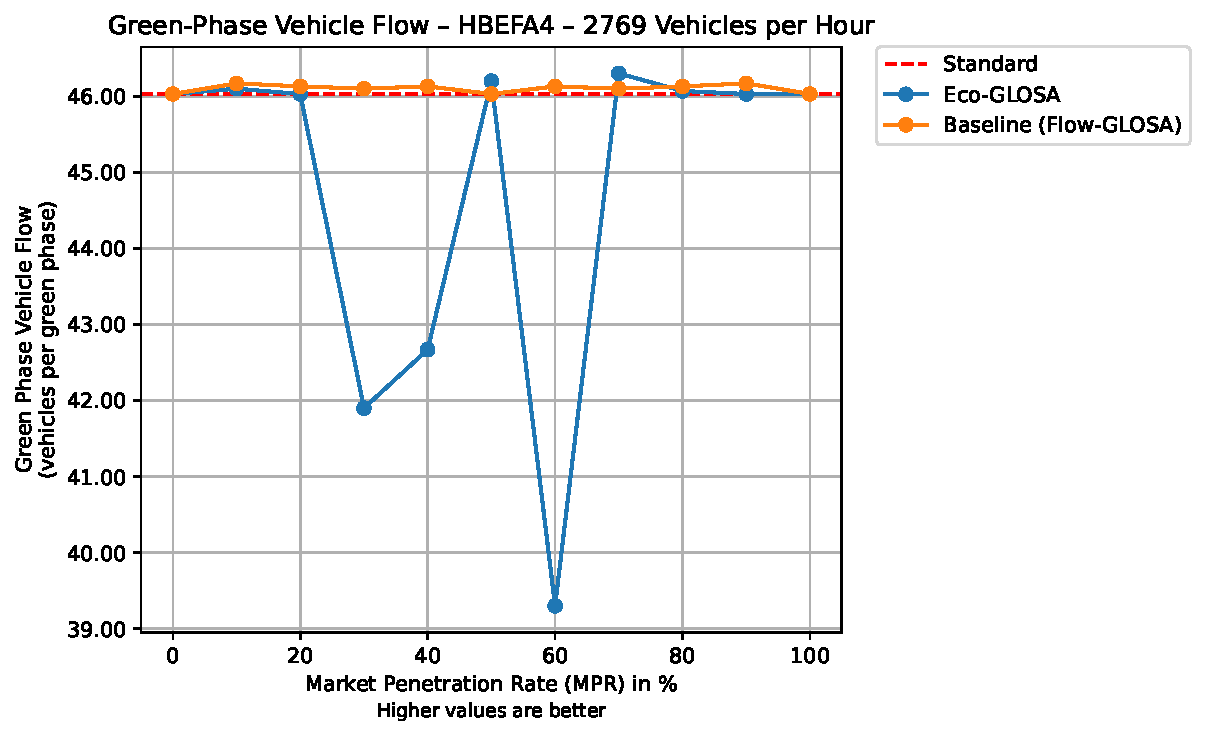
\includegraphics[width=0.49\textwidth]{data/img/GreenPhaseVehicleFlow/GreenPhaseVehicleFlow_HBEFA4_Cars2000.pdf}
  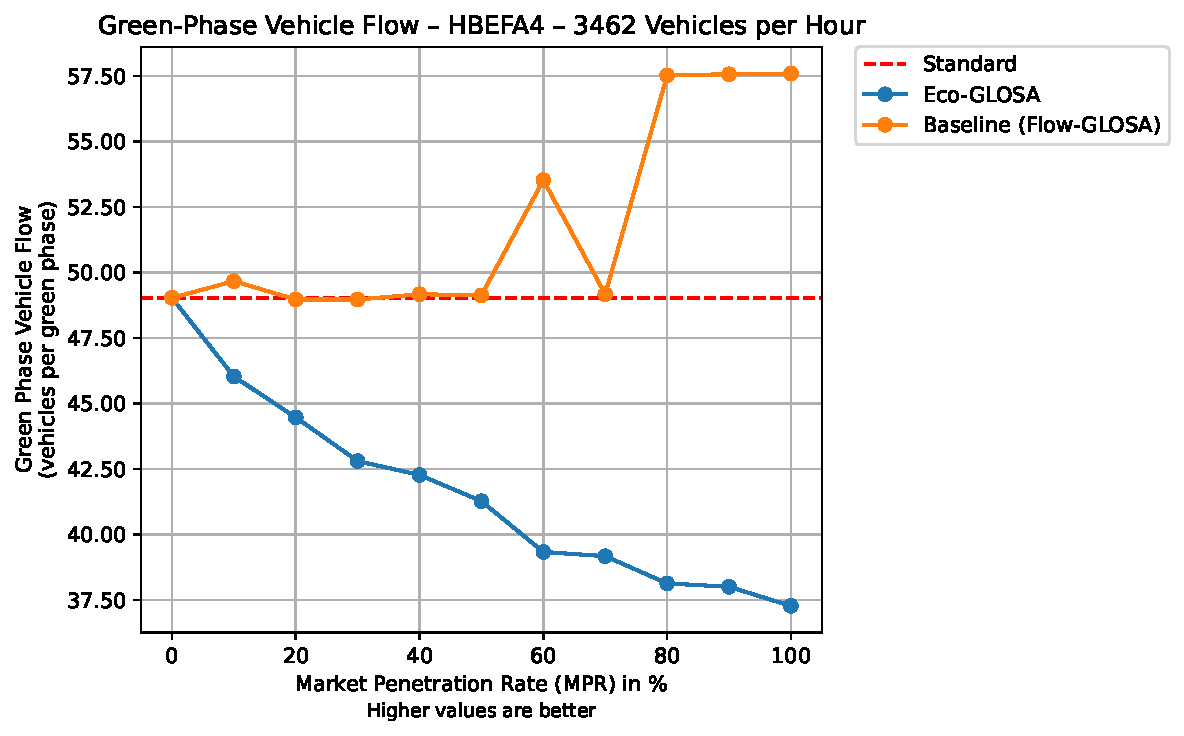
\includegraphics[width=0.49\textwidth]{data/img/GreenPhaseVehicleFlow/GreenPhaseVehicleFlow_HBEFA4_Cars2500.pdf}
  \caption[Green-phase vehicle flow vs. \ac{mpr} at $2077$, $2769$, and $3462~\unit{\veh\per\hour}$ (HBEFA4)]{Green-phase vehicle flow as a function of \ac{mpr} for three high-demand scenarios under the HBEFA4 emission model. The plots compare the performance of the Standard (no \ac{glosa}), \ac{eco-glosa}, and \ac{flow-glosa} controllers at demand levels of $2077$, $2769$, and $3462~\unit{\veh\per\hour}$.}
\label{fig:HBEFA4_Flow}
\end{figure}

\begin{figure}[htb]
  \centering
  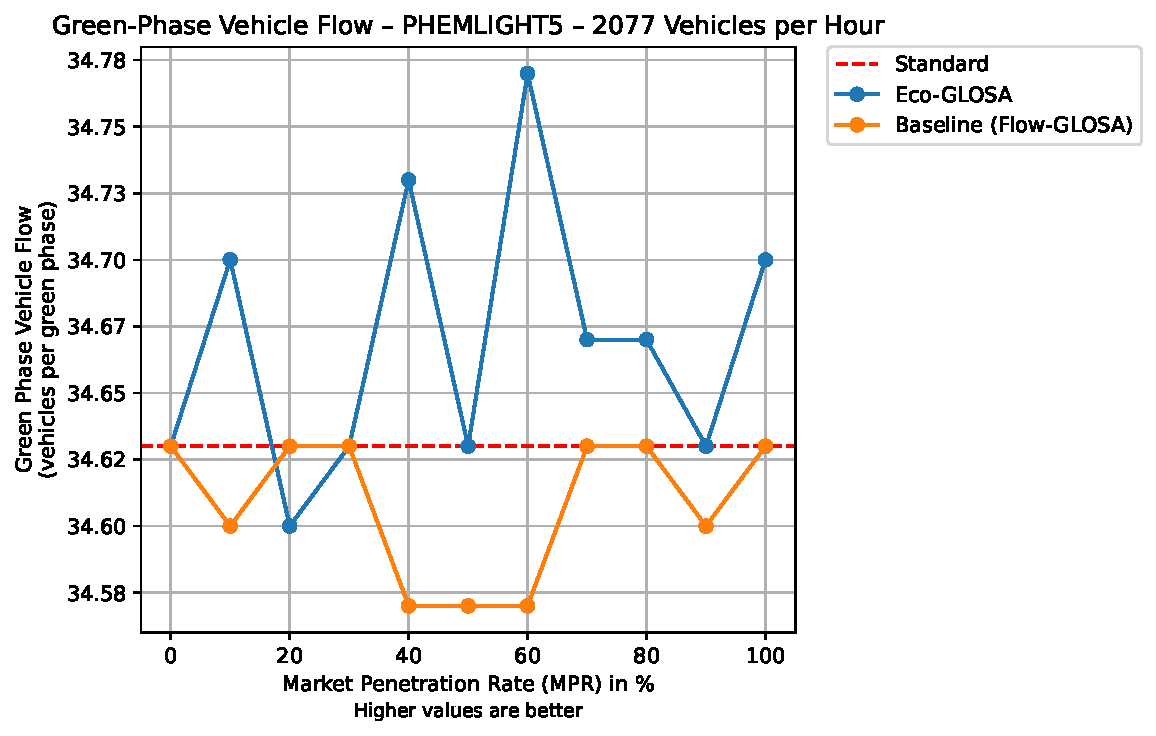
\includegraphics[width=0.49\textwidth]{data/img/GreenPhaseVehicleFlow/GreenPhaseVehicleFlow_PHEMLIGHT5_Cars1500.pdf}
  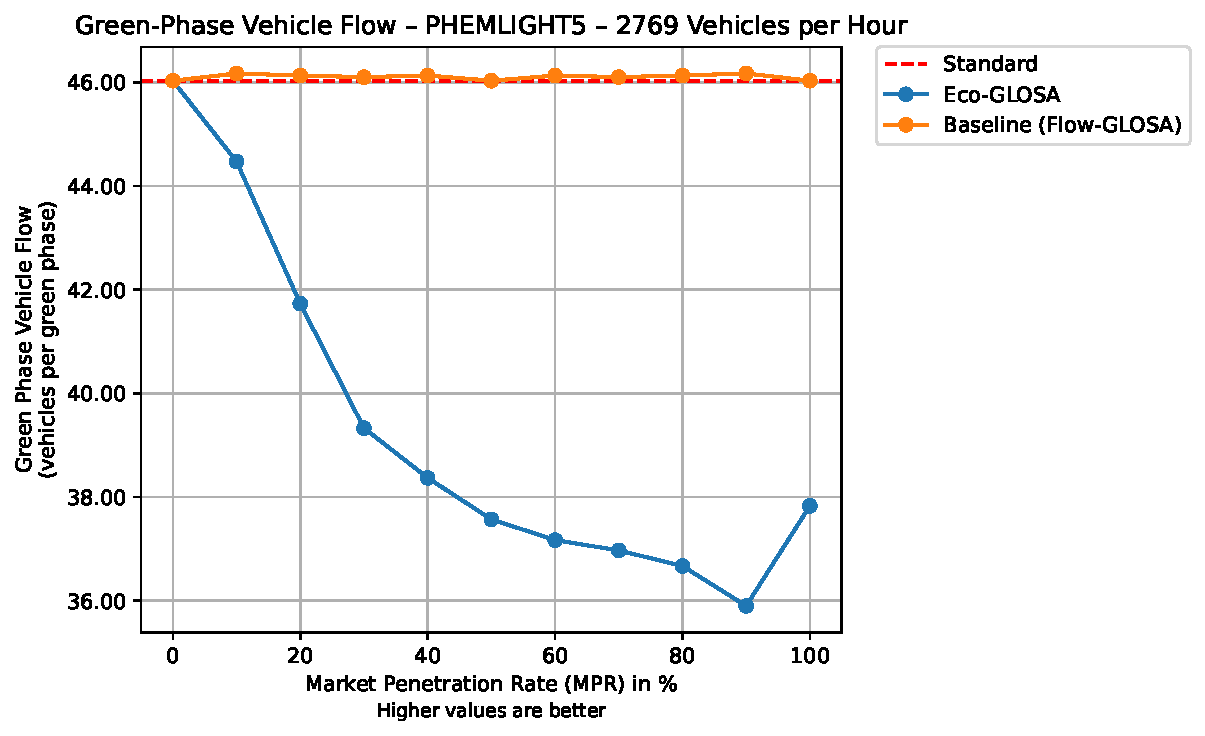
\includegraphics[width=0.49\textwidth]{data/img/GreenPhaseVehicleFlow/GreenPhaseVehicleFlow_PHEMLIGHT5_Cars2000.pdf}
  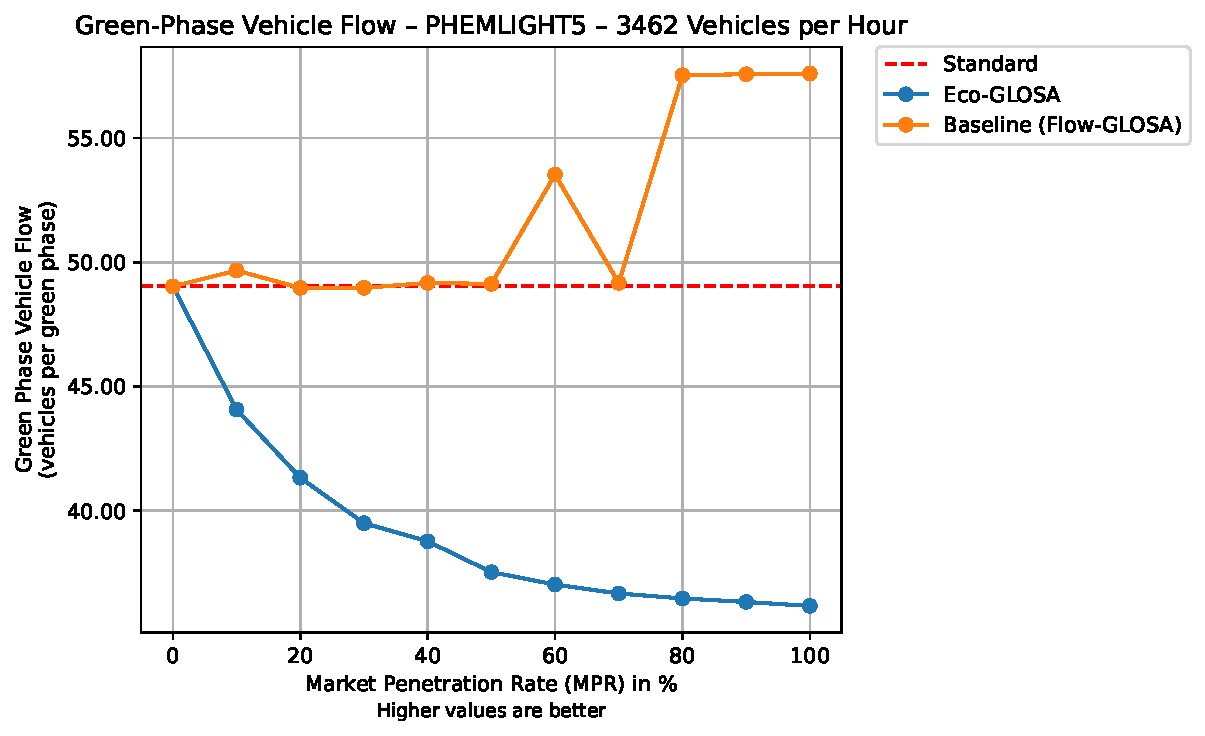
\includegraphics[width=0.49\textwidth]{data/img/GreenPhaseVehicleFlow/GreenPhaseVehicleFlow_PHEMLIGHT5_Cars2500.pdf}
  \caption[Green-phase vehicle flow vs. \ac{mpr} at $2077$, $2769$, and $3462~\unit{\veh\per\hour}$ (PHEMlight5)]{Green-phase vehicle flow as a function of \ac{mpr} for three high-demand scenarios under the PHEMlight5 emission model. The plots compare the performance of the Standard (no \ac{glosa}), \ac{eco-glosa}, and \ac{flow-glosa} controllers at demand levels of $2077$, $2769$, and $3462~\unit{\veh\per\hour}$.}
\label{fig:PHEM_Flow}
\end{figure}

\begin{table}[htb]
  \centering
  \caption[Green-phase vehicle throughput for all volumes and \ac{mpr} values]{Green-phase vehicle throughput, measured in vehicles per cycle, across all simulated traffic volumes and \ac{mpr} values. The Standard scenario denotes uncontrolled traffic ($0\%$ \ac{mpr}), while Baseline refers to the \ac{flow-glosa} controller.}
  \label{tab:GreenPhaseFlow}
  \resizebox{\textwidth}{!}{%
  \begin{tabular}{r l l r *{10}{r}}
    \toprule
    Vehicles & Algorithm                   & Fuel Model       & \textbf{0\% (Standard)} & 10\%  & 20\%  & 30\%  & 40\%  & 50\%  & 60\%  & 70\%  & 80\%  & 90\%  & 100\% \\
    \midrule
    69   & \ac{eco-glosa}              & HBEFA4           & \textbf{1.17} & 1.17  & 1.17  & 1.17  & 1.17  & 1.13  & 1.17  & 1.17  & 1.13  & 1.17  & 1.17  \\
    69   & Baseline (\ac{flow-glosa})  & HBEFA4           & \textbf{1.17} & 1.17  & 1.17  & 1.17  & 1.17  & 1.13  & 1.17  & 1.17  & 1.17  & 1.17  & 1.17  \\
    69   & \ac{eco-glosa}              & PHEMLIGHT5       & \textbf{1.17} & 1.17  & 1.17  & 1.17  & 1.17  & 1.13  & 1.17  & 1.17  & 1.17  & 1.17  & 1.17  \\
    69   & Baseline (\ac{flow-glosa})  & PHEMLIGHT5       & \textbf{1.17} & 1.17  & 1.17  & 1.17  & 1.17  & 1.13  & 1.17  & 1.17  & 1.17  & 1.17  & 1.17  \\
    \midrule
    138  & \ac{eco-glosa}              & HBEFA4           & \textbf{2.30} & 2.30  & 2.30  & 2.27  & 2.27  & 2.27  & 2.27  & 2.30  & 2.30  & 2.27  & 2.27  \\
    138  & Baseline (\ac{flow-glosa})  & HBEFA4           & \textbf{2.30} & 2.30  & 2.30  & 2.30  & 2.27  & 2.27  & 2.27  & 2.30  & 2.30  & 2.30  & 2.30  \\
    138  & \ac{eco-glosa}              & PHEMLIGHT5       & \textbf{2.30} & 2.30  & 2.30  & 2.27  & 2.27  & 2.27  & 2.27  & 2.30  & 2.30  & 2.30  & 2.27  \\
    138  & Baseline (\ac{flow-glosa})  & PHEMLIGHT5       & \textbf{2.30} & 2.30  & 2.30  & 2.30  & 2.27  & 2.27  & 2.27  & 2.30  & 2.30  & 2.30  & 2.30  \\
    \midrule
    346  & \ac{eco-glosa}              & HBEFA4           & \textbf{5.73} & 5.70  & 5.77  & 5.73  & 5.73  & 5.77  & 5.73  & 5.73  & 5.73  & 5.70  & 5.73  \\
    346  & Baseline (\ac{flow-glosa})  & HBEFA4           & \textbf{5.73} & 5.73  & 5.73  & 5.70  & 5.73  & 5.73  & 5.73  & 5.70  & 5.73  & 5.73  & 5.73  \\
    346  & \ac{eco-glosa}              & PHEMLIGHT5       & \textbf{5.73} & 5.73  & 5.73  & 5.70  & 5.77  & 5.73  & 5.73  & 5.70  & 5.70  & 5.70  & 5.77  \\
    346  & Baseline (\ac{flow-glosa})  & PHEMLIGHT5       & \textbf{5.73} & 5.73  & 5.73  & 5.70  & 5.73  & 5.73  & 5.73  & 5.70  & 5.73  & 5.73  & 5.73  \\
    \midrule
    692  & \ac{eco-glosa}              & HBEFA4           & \textbf{11.57} & 11.60 & 11.57 & 11.57 & 11.60 & 11.57 & 11.57 & 11.57 & 11.57 & 11.53 & 11.63 \\
    692  & Baseline (\ac{flow-glosa})  & HBEFA4           & \textbf{11.57} & 11.60 & 11.60 & 11.60 & 11.60 & 11.60 & 11.60 & 11.60 & 11.60 & 11.60 & 11.57 \\
    692  & \ac{eco-glosa}              & PHEMLIGHT5       & \textbf{11.57} & 11.57 & 11.53 & 11.53 & 11.57 & 11.57 & 11.60 & 11.57 & 11.50 & 11.53 & 11.63 \\
    692  & Baseline (\ac{flow-glosa})  & PHEMLIGHT5       & \textbf{11.57} & 11.60 & 11.60 & 11.60 & 11.60 & 11.60 & 11.60 & 11.60 & 11.60 & 11.60 & 11.57 \\
    \midrule
    1385 & \ac{eco-glosa}              & HBEFA4           & \textbf{23.03} & 22.97 & 23.07 & 22.97 & 23.03 & 23.10 & 23.03 & 23.03 & 22.97 & 23.07 & 23.03 \\
    1385 & Baseline (\ac{flow-glosa})  & HBEFA4           & \textbf{23.03} & 23.13 & 23.10 & 23.07 & 23.03 & 23.10 & 23.03 & 23.07 & 23.10 & 23.13 & 23.03 \\
    1385 & \ac{eco-glosa}              & PHEMLIGHT5       & \textbf{23.03} & 23.07 & 23.03 & 23.03 & 23.10 & 23.07 & 23.07 & 22.93 & 22.93 & 23.00 & 23.03 \\
    1385 & Baseline (\ac{flow-glosa})  & PHEMLIGHT5       & \textbf{23.03} & 23.13 & 23.10 & 23.07 & 23.03 & 23.10 & 23.03 & 23.07 & 23.10 & 23.13 & 23.03 \\
    \midrule
    2077 & \ac{eco-glosa}              & HBEFA4           & \textbf{34.63} & 34.70 & 34.67 & 34.63 & 34.67 & 34.63 & 34.70 & 34.63 & 34.63 & 34.63 & 34.67 \\
    2077 & Baseline (\ac{flow-glosa})  & HBEFA4           & \textbf{34.63} & 34.60 & 34.63 & 34.63 & 34.57 & 34.57 & 34.57 & 34.63 & 34.63 & 34.60 & 34.63 \\
    2077 & \ac{eco-glosa}              & PHEMLIGHT5       & \textbf{34.63} & 34.70 & 34.60 & 34.63 & 34.73 & 34.63 & 34.77 & 34.67 & 34.67 & 34.63 & 34.70 \\
    2077 & Baseline (\ac{flow-glosa})  & PHEMLIGHT5       & \textbf{34.63} & 34.60 & 34.63 & 34.63 & 34.57 & 34.57 & 34.57 & 34.63 & 34.63 & 34.60 & 34.63 \\
    \midrule
    2769 & Eco-\ac{eco-glosa}           & HBEFA4         & \textbf{46.03} & 46.10 & 46.03 & 41.90 & 42.67 & 46.20 & 39.30 & 46.30 & 46.07 & 46.03 & 46.03 \\
    2769 & Baseline (\ac{flow-glosa})   & HBEFA4         & \textbf{46.03} & 46.17 & 46.13 & 46.10 & 46.13 & 46.03 & 46.13 & 46.10 & 46.13 & 46.17 & 46.03 \\
    \textbf{2769} & \textbf{\ac{eco-glosa}} & \textbf{PHEMLIGHT5} & \textbf{46.03} & \textbf{44.47} & \textbf{41.73} & \textbf{39.33} & \textbf{38.37} & \textbf{37.57} & \textbf{37.17} & \textbf{36.97} & \textbf{36.67} & \textbf{35.90} & \textbf{37.83} \\
    2769 & Baseline (\ac{flow-glosa})  & PHEMLIGHT5       & \textbf{46.03} & 46.17 & 46.13 & 46.10 & 46.13 & 46.03 & 46.13 & 46.10 & 46.13 & 46.17 & 46.03 \\
    \midrule
    \textbf{3462} & \textbf{\ac{eco-glosa}} & \textbf{HBEFA4}   & \textbf{49.03} & \textbf{46.03} & \textbf{44.47} & \textbf{42.80} & \textbf{42.27} & \textbf{41.27} & \textbf{39.33} & \textbf{39.17} & \textbf{38.13} & \textbf{38.00} & \textbf{37.27} \\
    3462 & Baseline (\ac{flow-glosa})  & HBEFA4           & \textbf{49.03} & 49.07 & 48.83 & 49.53 & 48.97 & 49.23 & 48.97 & 49.53 & 48.83 & 49.07 & 49.03 \\
    \textbf{3462} & \textbf{\ac{eco-glosa}} & \textbf{PHEMLIGHT5} & \textbf{49.03} & \textbf{44.07} & \textbf{41.33} & \textbf{39.50} & \textbf{38.77} & \textbf{37.53} & \textbf{37.03} & \textbf{36.67} & \textbf{36.47} & \textbf{36.33} & \textbf{36.17} \\
    3462 & Baseline (\ac{flow-glosa})  & PHEMLIGHT5       & \textbf{49.03} & 49.07 & 48.83 & 49.53 & 48.97 & 49.23 & 48.97 & 49.53 & 48.83 & 49.07 & 49.03 \\
    \bottomrule
  \end{tabular}%
  }
\end{table}

\section{Average Vehicle Speed}
\label{sec:Results_MeanSpeed}

Table~\ref{tab:MeanSpeed} and Figures~\ref{fig:MeanSpeed_2077}–\ref{fig:MeanSpeed_3462} report the mean cruise speed of the platoon as a function of \ac{mpr}. The three control strategies, Standard, \ac{eco-glosa} and \ac{flow-glosa}, are compared under both emission models (HBEFA4 and PHEMLIGHT5) at three critical demand levels. A careful examination of the data yields six principal insights.

\subparagraph*{1. Systematic impact of \ac{mpr} on \ac{eco-glosa}.}
Across \emph{all} volumes, \ac{eco-glosa} shows a monotonic speed decrease as \ac{mpr} increases. For example, at the lightest load of $69\,\mathrm{veh/h}$, the HBEFA4 mean speed drops from $13.34\,\mathrm{m/s}$ (Standard) to $13.01\,\mathrm{m/s}$ at $100\,\%$ \ac{mpr} ($\downarrow 2.5\,\%$). The reduction accelerates with demand: at $2077\,\mathrm{veh/h}$, the decrease is $0.44\,\mathrm{m/s}$ ($\downarrow 3.5\,\%$) by $40\,\%$ \ac{mpr}, while at $2769\,\mathrm{veh/h}$ it becomes catastrophic, falling from $11.94\,\mathrm{m/s}$ to $2.57\,\mathrm{m/s}$ ($\downarrow 79\,\%$) by $90\,\%$ \ac{mpr} under PHEMlight5 (Figure~\ref{fig:MeanSpeed_PHEM_2769}). This monotonic decline is, for example, illustrated in Figures~\ref{fig:MeanSpeed_HBEFA4_2077} and~\ref{fig:MeanSpeed_PHEM_2077}.

\subparagraph*{2. Flow stability and jam resolution of \ac{flow-glosa}.}
\ac{flow-glosa} maintains near-Standard speeds up to $2769\,\mathrm{veh/h}$, and under full saturation ($3462\,\mathrm{veh/h}$) it dissolves the queue once penetration exceeds approximately $80\%$. The mean speed increases from $\mathbf{3.86\,\mathrm{m/s}}$ (Standard, 0\% \ac{mpr}) to $4.16\,\mathrm{m/s}$ at $50\%$ \ac{mpr} and ultimately reaches $\mathbf{12.18\,\mathrm{m/s}}$ at $100\%$ \ac{mpr}. This behaviour demonstrates that \ac{flow-glosa} can actively resolve gridlock and restore free-flow speeds when a sufficient share of vehicles conforms to its advisory. The jam-dissolving capability is evident in Figures~\ref{fig:MeanSpeed_HBEFA4_3462} and~\ref{fig:MeanSpeed_PHEM_3462}.  


\subparagraph*{3. Emission-model sensitivity.}
PHEMlight5 consistently produces lower speeds than HBEFA4 at the same \ac{mpr} and demand level. The difference is modest at low demand (approximately $0.1\,\mathrm{m/s}$ for $69$--$346\,\mathrm{veh/h}$) but widens dramatically in congestion. At $2769\,\mathrm{veh/h}$ and $30\,\%$ \ac{mpr}, PHEMlight5--\ac{eco-glosa} already drops to $3.17\,\mathrm{m/s}$ versus $7.32\,\mathrm{m/s}$ for HBEFA4, a $57\,\%$ gap. This reflects the higher temporal resolution and the non-linear fuel--speed polynomial in PHEMlight5: it penalises short bursts of high engine power more strongly, which prompts earlier decelerations and thus longer queuing times. The widening gap between HBEFA4 and PHEMlight5 under congestion is visible in Figures~\ref{fig:MeanSpeed_HBEFA4_2769} and~\ref{fig:MeanSpeed_PHEM_2769}.

\subparagraph*{4. Jam-onset thresholds.}
Under the conventional jam criterion of around $v \leq 4\,\mathrm{m/s}$ in urban areas, Table~\ref{tab:MeanSpeed} reveals discrete breakpoints for the \ac{eco-glosa}. In the PHEMlight5 case, a jam forms at $10$--$20\,\%$ \ac{mpr} for $2769\,\mathrm{veh/h}$ and at the first non-zero \ac{mpr} for $3462\,\mathrm{veh/h}$. HBEFA4 postpones the jam onset by roughly one \ac{mpr} decade: $30$--$50\,\%$ at $2769\,\mathrm{veh/h}$. The staggered thresholds underscore the importance of the emission-model choice when extrapolating eco-driving benefits to congested corridors. The onset of jam (v\,$\le4\,\mathrm{m/s}$) corresponds to the inflection points in Figures~\ref{fig:MeanSpeed_HBEFA4_2769} and~\ref{fig:MeanSpeed_PHEM_2769}.

\subparagraph*{5. Residual overshoot at low demand.}
At sub-saturated volumes ($69$--$1385\,\mathrm{veh/h}$), \ac{eco-glosa} occasionally overshoots Standard by up to $0.04\,\mathrm{m/s}$ at $10\,\%$ \ac{mpr}. The effect, most visible in HBEFA4, originates from the algorithm's \enquote{anticipatory glide} that smooths minor stop-and-go waves, thereby shortening braking phases and slightly increasing the arithmetic mean of cruise speed. However, as soon as \ac{mpr} exceeds approximately $20\,\%$, the fuel-saving bias dominates and the curve bends downward. The slight overshoot at low demand (10\,\% \ac{mpr}) is observable in Figures~\ref{fig:MeanSpeed_HBEFA4_2077} and~\ref{fig:MeanSpeed_PHEM_2077}.

\subparagraph*{6. Progressive speed gains under \ac{flow-glosa}.}
As \ac{mpr} increases, \ac{flow-glosa} delivers measurable speed improvements even below saturation. At low demand ($69\,\mathrm{veh/h}$), HBEFA4–\ac{flow-glosa} speeds climb from $\mathbf{13.34}$ to $13.88\,\mathrm{m/s}$ ($+4.1\,\%$) by $90\,\%$ \ac{mpr}. At medium demand ($1385\,\mathrm{veh/h}$), the mean speed rises from $\mathbf{12.84}$ to $13.07\,\mathrm{m/s}$ ($+1.8\,\%$) at $100\,\%$ penetration. Even at high demand ($2769\,\mathrm{veh/h}$), it increases from $\mathbf{11.94}$ to $12.55\,\mathrm{m/s}$ ($+5.1\,\%$) at $100\,\%$ \ac{mpr}. These consistent gains underscore \ac{flow-glosa}’s capacity to smooth stop-and-go waves and improve throughput across light, moderate, and heavy traffic regimes. The progressive uplift with increasing penetration is shown by the upward slopes in Figures~\ref{fig:MeanSpeed_HBEFA4_2077}, \ref{fig:MeanSpeed_HBEFA4_2769}, and \ref{fig:MeanSpeed_HBEFA4_3462} (and similarly for PHEMLIGHT5 in Figures~\ref{fig:MeanSpeed_PHEM_2077}, \ref{fig:MeanSpeed_PHEM_2769}, \ref{fig:MeanSpeed_PHEM_3462}).

\begin{figure}[htb]
  \centering
  \begin{subfigure}[b]{0.49\textwidth}
    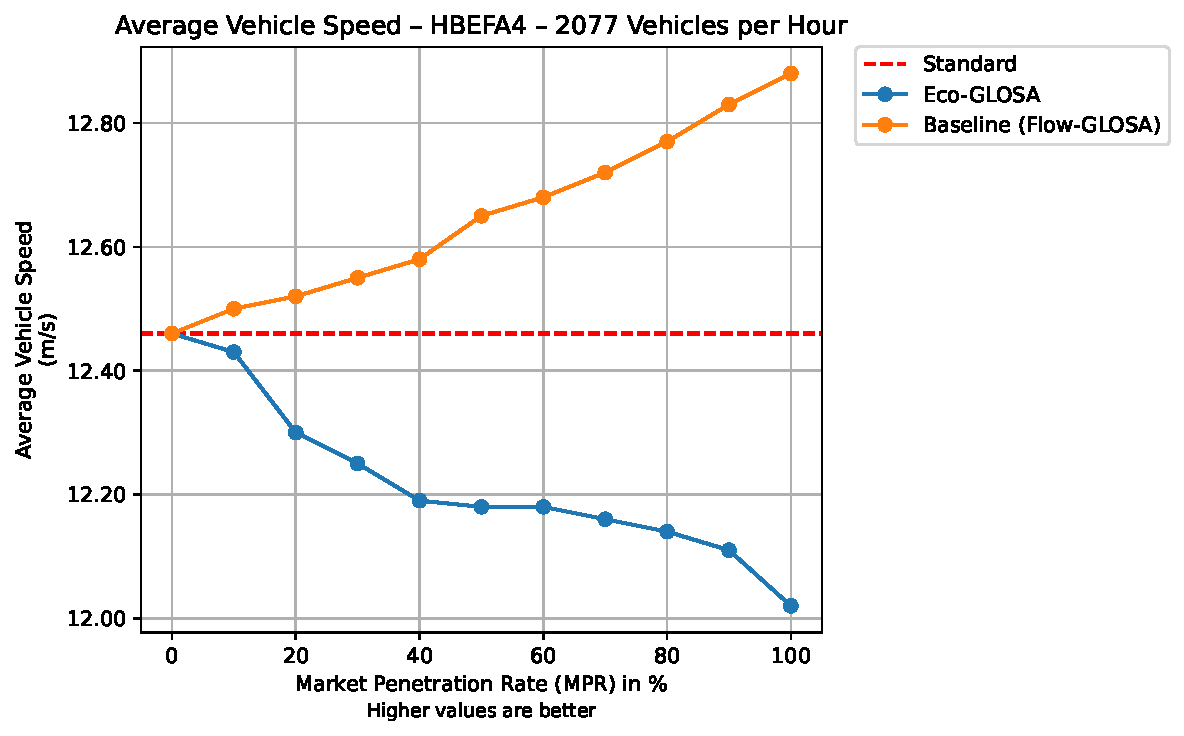
\includegraphics[width=\textwidth]{data/img/AverageVehicleSpeed/AverageVehicleSpeed_HBEFA4_Cars2077.pdf}
    \caption{Mean vehicle speed as a function of \ac{mpr} for the HBEFA4 emission model at a demand level of $2077\,\mathrm{veh/h}$.}
    \label{fig:MeanSpeed_HBEFA4_2077}
  \end{subfigure}\hfill
  \begin{subfigure}[b]{0.49\textwidth}
    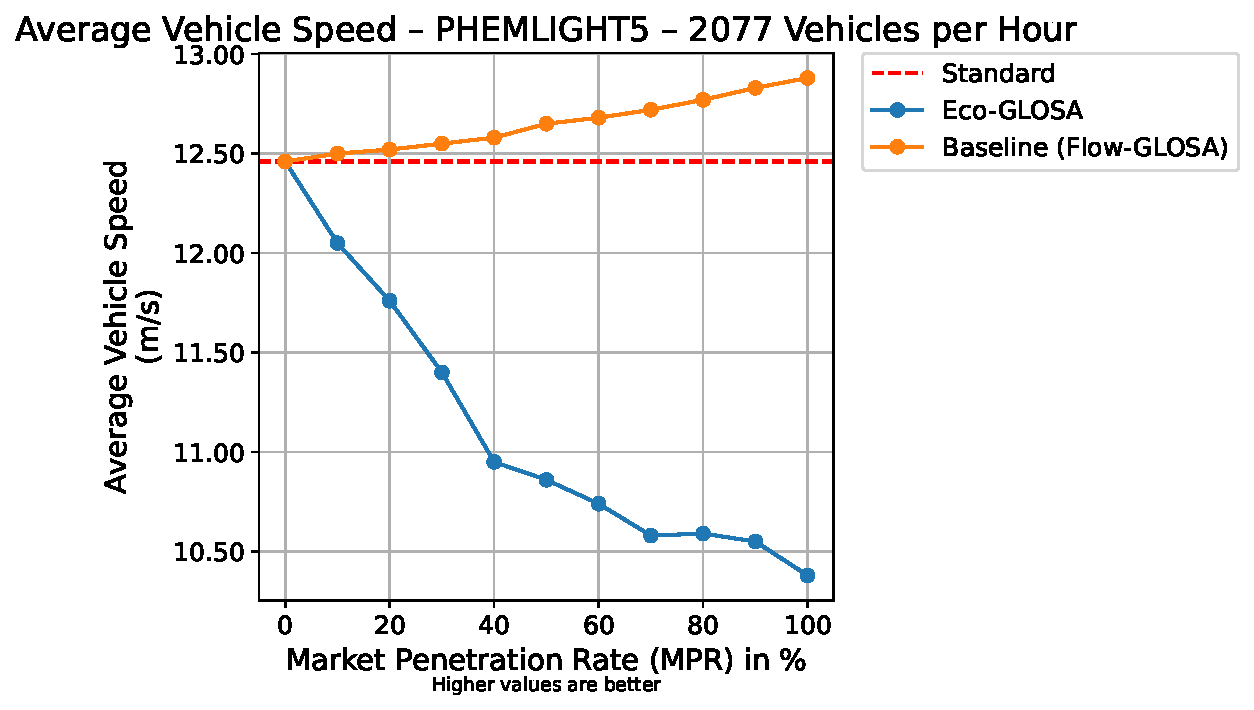
\includegraphics[width=\textwidth]{data/img/AverageVehicleSpeed/AverageVehicleSpeed_PHEMLIGHT5_Cars2077.pdf}
    \caption{Mean vehicle speed as a function of \ac{mpr} for the PHEMlight5 emission model at a demand level of $2077\,\mathrm{veh/h}$.}
    \label{fig:MeanSpeed_PHEM_2077}
  \end{subfigure}
  \caption{Mean vehicle speed as a function of \ac{mpr} at $2077\,\mathrm{veh/h}$ for the HBEFA4 and PHEMlight5 emission models. The plots show results for the Standard, \ac{eco-glosa}, and \ac{flow-glosa} algorithms.}
  \label{fig:MeanSpeed_2077}
\end{figure}


\begin{figure}[htb]
  \centering
  \begin{subfigure}[b]{0.49\textwidth}
    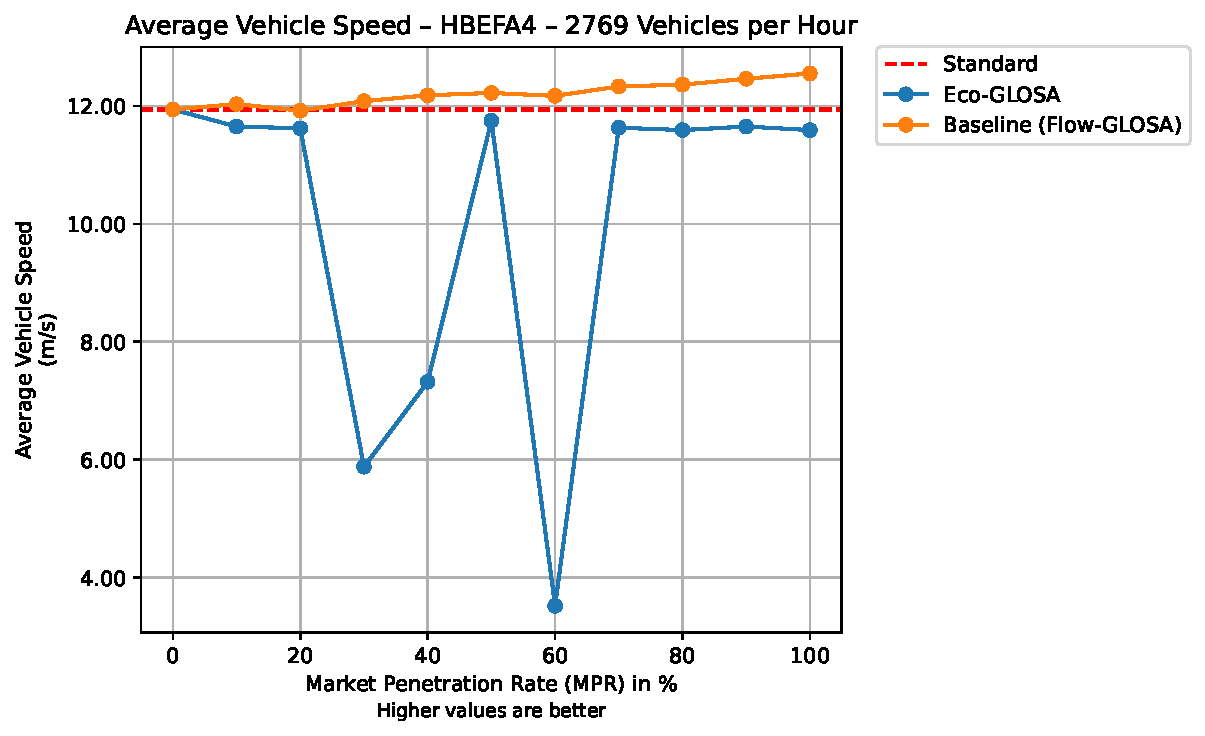
\includegraphics[width=\textwidth]{data/img/AverageVehicleSpeed/AverageVehicleSpeed_HBEFA4_Cars2769.pdf}
    \caption{Mean vehicle speed as a function of \ac{mpr} for the HBEFA4 emission model at $2769\,\mathrm{veh/h}$.}
    \label{fig:MeanSpeed_HBEFA4_2769}
  \end{subfigure}\hfill
  \begin{subfigure}[b]{0.49\textwidth}
    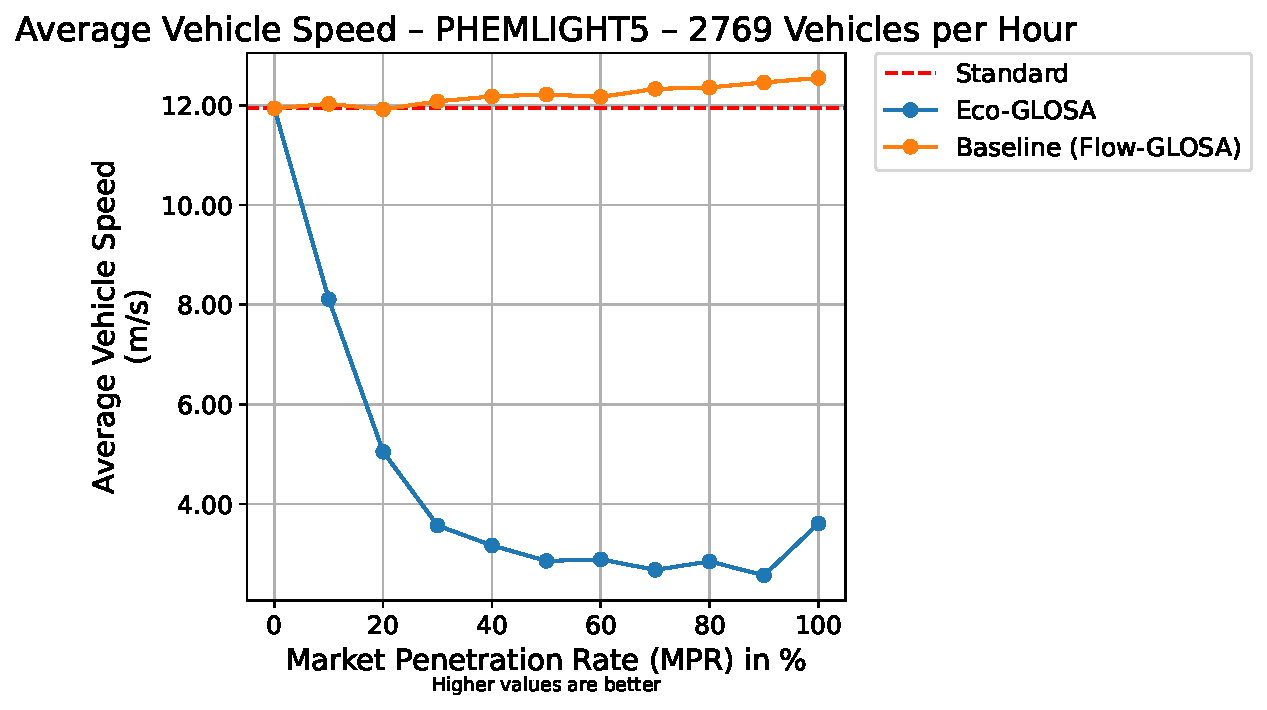
\includegraphics[width=\textwidth]{data/img/AverageVehicleSpeed/AverageVehicleSpeed_PHEMLIGHT5_Cars2769.pdf}
    \caption{Mean vehicle speed as a function of \ac{mpr} for the PHEMlight5 emission model at $2769\,\mathrm{veh/h}$.}
    \label{fig:MeanSpeed_PHEM_2769}
  \end{subfigure}
  \caption{Mean vehicle speed as a function of \ac{mpr} at $2769\,\mathrm{veh/h}$ for the HBEFA4 and PHEMlight5 emission models. The results include the Standard, \ac{eco-glosa}, and \ac{flow-glosa} algorithms.}
  \label{fig:MeanSpeed_2769}
\end{figure}

\begin{figure}[htb]
  \centering
  \begin{subfigure}[b]{0.49\textwidth}
    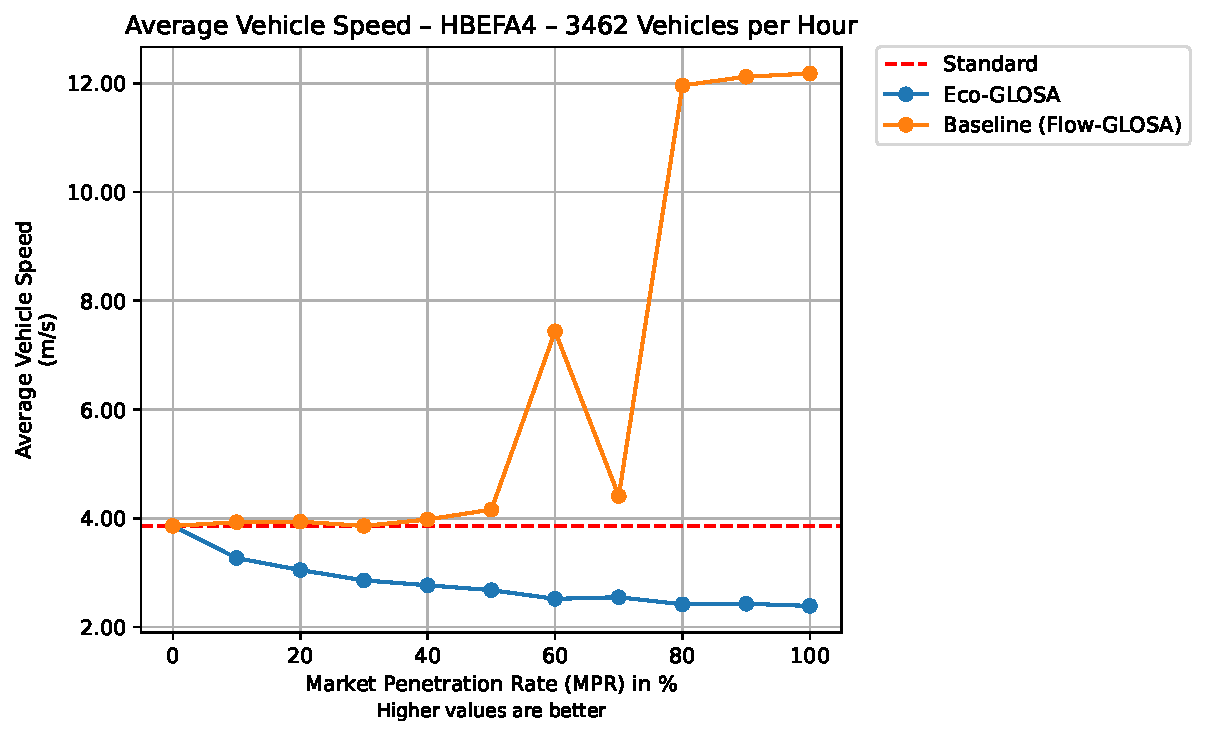
\includegraphics[width=\textwidth]{data/img/AverageVehicleSpeed/AverageVehicleSpeed_HBEFA4_Cars3462.pdf}
    \caption{Mean vehicle speed as a function of \ac{mpr} for the HBEFA4 emission model at $3462\,\mathrm{veh/h}$.}
    \label{fig:MeanSpeed_HBEFA4_3462}
  \end{subfigure}\hfill
  \begin{subfigure}[b]{0.49\textwidth}
    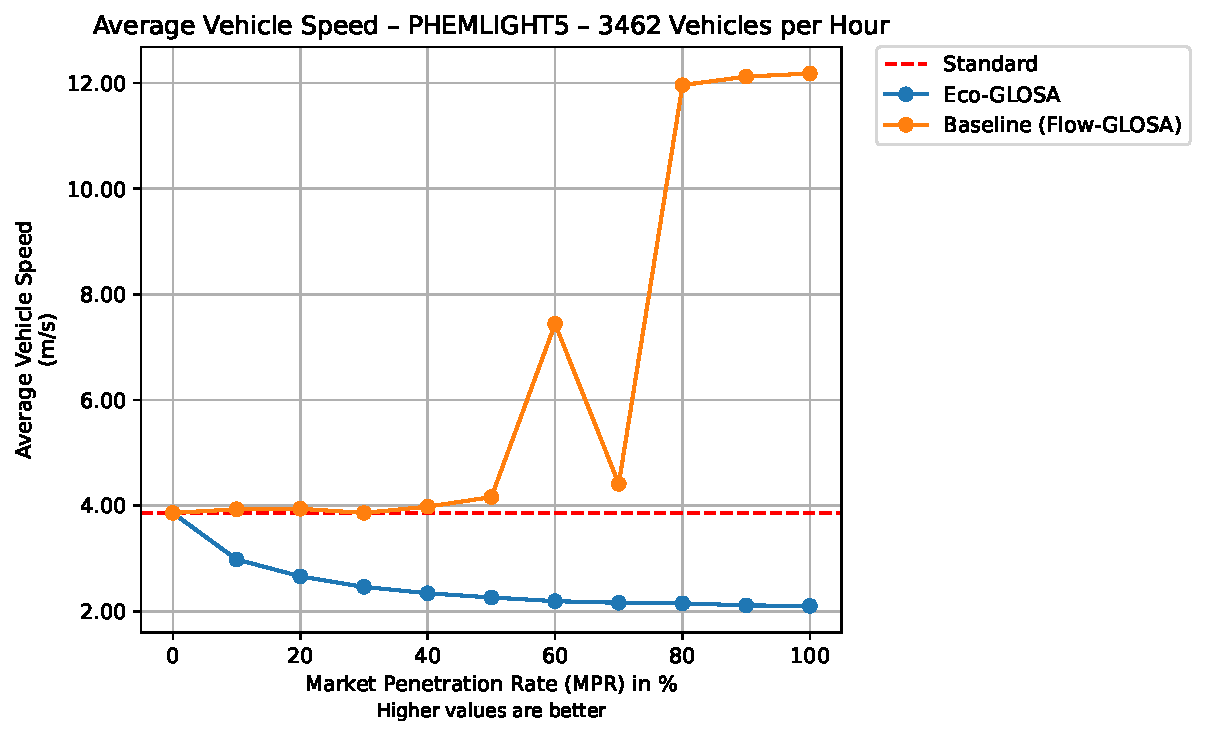
\includegraphics[width=\textwidth]{data/img/AverageVehicleSpeed/AverageVehicleSpeed_PHEMLIGHT5_Cars3462.pdf}
    \caption{Mean vehicle speed as a function of \ac{mpr} for the PHEMlight5 emission model at $3462\,\mathrm{veh/h}$.}
    \label{fig:MeanSpeed_PHEM_3462}
  \end{subfigure}
  \caption{Mean vehicle speed as a function of \ac{mpr} at $3462\,\mathrm{veh/h}$ for the HBEFA4 and PHEMlight5 emission models. The results are shown for the Standard, \ac{eco-glosa}, and \ac{flow-glosa} algorithms.}
  \label{fig:MeanSpeed_3462}
\end{figure}

\subparagraph*{Implications.}
\ac{flow-glosa}’s advisory logic is agnostic to the emission model, so its speed curves coincide exactly for HBEFA4 and PHEMLIGHT5 (see Figures~\ref{fig:MeanSpeed_HBEFA4_2077} and~\ref{fig:MeanSpeed_PHEM_2077}). By contrast, \ac{eco-glosa} computes its target speeds using the specific fuel model, yielding markedly different slowdowns: under PHEMLIGHT5 the mean speed at $2077\,\mathrm{veh/h}$ begins to fall at only $10\%$ \ac{mpr} (Figure~\ref{fig:MeanSpeed_PHEM_2077}), whereas under HBEFA4 the speed remains within $0.1\,\mathrm{m/s}$ of Standard until $30\%$ \ac{mpr} (Figure~\ref{fig:MeanSpeed_HBEFA4_2077}). Once the junction saturates ($3462\,\mathrm{veh/h}$), \ac{flow-glosa} can actually dissolve the queue at high \ac{mpr}, restoring free-flow speeds above $12\,\mathrm{m/s}$ (Figures~\ref{fig:MeanSpeed_HBEFA4_3462} and~\ref{fig:MeanSpeed_PHEM_3462}), whereas \ac{eco-glosa} remains gridlocked. At light to moderate volumes ($69$–$1385\,\mathrm{veh/h}$), \ac{eco-glosa} still offers marginal smoothing of stop-and-go oscillations, occasionally exceeding Standard by up to $0.04\,\mathrm{m/s}$ at $10\%$ \ac{mpr} (Figures~\ref{fig:MeanSpeed_HBEFA4_2077} and~\ref{fig:MeanSpeed_PHEM_2077}), but these gains vanish as \ac{mpr} exceeds $20\%$. Therefore, on lightly loaded arterials \ac{eco-glosa} may be deployed to fine-tune speed consistency, while on corridors operating near or above $2077\,\mathrm{veh/h}$ \ac{flow-glosa} is essential to maintain throughput, prevent premature queuing, and even resolve existing gridlock.

\begin{table}[htb]
  \centering
  \caption{Mean vehicle speed in meters per second ($\mathrm{m/s}$) as a function of traffic demand and \ac{mpr} for the different algorithm configurations. Outcomes are provided for the Baseline configuration (\ac{flow-glosa}), the Eco configuration (\ac{eco-glosa}), and the Standard case (no \ac{glosa}, $0\,\%$ \ac{mpr}).}
  \label{tab:MeanSpeed}
  \resizebox{\textwidth}{!}{%
  \begin{tabular}{r l l r *{10}{r}}
    \toprule
    Cars & Algorithm & Fuel & \textbf{0\% (Std)} & 10\% & 20\% & 30\% & 40\% & 50\% & 60\% & 70\% & 80\% & 90\% & 100\%\\
    \midrule
    69  & \ac{eco-glosa} & HBEFA4 & \textbf{13.34} & 13.86 & 13.45 & 13.71 & 13.51 & 13.46 & 13.71 & 13.72 & 13.05 & 13.81 & 13.01\\
    69  & Baseline (\ac{flow-glosa}) & HBEFA4 & \textbf{13.34} & 13.98 & 13.58 & 13.66 & 13.69 & 13.62 & 13.65 & 13.85 & 13.63 & 13.88 & 13.34\\
    69  & \ac{eco-glosa} & PHEMLIGHT5 & \textbf{13.34} & 13.89 & 13.38 & 13.79 & 13.60 & 12.77 & 13.30 & 13.23 & 12.81 & 13.70 & 12.34\\
    69  & Baseline (\ac{flow-glosa}) & PHEMLIGHT5 & \textbf{13.34} & 13.98 & 13.58 & 13.66 & 13.69 & 13.62 & 13.65 & 13.85 & 13.63 & 13.88 & 13.34\\
    \midrule
    138 & \ac{eco-glosa} & HBEFA4 & \textbf{13.24} & 13.51 & 13.29 & 13.46 & 13.56 & 13.36 & 13.52 & 13.17 & 13.12 & 13.01 & 12.97\\
    138 & Baseline (\ac{flow-glosa}) & HBEFA4 & \textbf{13.24} & 13.52 & 13.37 & 13.41 & 13.65 & 13.47 & 13.57 & 13.52 & 13.41 & 13.39 & 13.23\\
    138 & \ac{eco-glosa} & PHEMLIGHT5 & \textbf{13.24} & 13.38 & 13.40 & 13.36 & 13.64 & 13.15 & 13.39 & 13.03 & 12.99 & 12.70 & 12.50\\
    138 & Baseline (\ac{flow-glosa}) & PHEMLIGHT5 & \textbf{13.24} & 13.52 & 13.37 & 13.41 & 13.65 & 13.47 & 13.57 & 13.52 & 13.41 & 13.39 & 13.23\\
    \midrule
    346 & \ac{eco-glosa} & HBEFA4 & \textbf{13.24} & 13.24 & 13.14 & 13.07 & 13.18 & 13.01 & 13.08 & 13.04 & 12.96 & 12.99 & 12.87\\
    346 & Baseline (\ac{flow-glosa}) & HBEFA4 & \textbf{13.24} & 13.27 & 13.19 & 13.20 & 13.25 & 13.28 & 13.33 & 13.33 & 13.35 & 13.36 & \textbf{13.48}\\
    346 & \ac{eco-glosa} & PHEMLIGHT5 & \textbf{13.24} & 13.20 & 12.83 & 12.71 & 12.80 & 12.77 & 12.56 & 12.59 & 12.52 & 12.64 & 12.50\\
    346 & Baseline (\ac{flow-glosa}) & PHEMLIGHT5 & \textbf{13.24} & 13.27 & 13.19 & 13.20 & 13.25 & 13.28 & 13.33 & 13.33 & 13.35 & 13.36 & \textbf{13.48}\\
    \midrule
    692 & \ac{eco-glosa} & HBEFA4 & \textbf{13.17} & 13.13 & 13.17 & 13.09 & 13.04 & 13.01 & 13.05 & 12.94 & 12.91 & 12.82 & 12.81\\
    692 & Baseline (\ac{flow-glosa}) & HBEFA4 & \textbf{13.17} & 13.23 & 13.25 & 13.20 & 13.27 & 13.22 & 13.36 & 13.25 & 13.31 & 13.39 & 13.33\\
    692 & \ac{eco-glosa} & PHEMLIGHT5 & \textbf{13.17} & 13.08 & 12.95 & 12.71 & 12.68 & 12.52 & 12.49 & 12.38 & 12.24 & 12.11 & 12.10\\
    692 & Baseline (\ac{flow-glosa}) & PHEMLIGHT5 & \textbf{13.17} & 13.23 & 13.25 & 13.20 & 13.27 & 13.22 & 13.36 & 13.25 & 13.31 & 13.39 & 13.33\\
    \midrule
    1385 & \ac{eco-glosa} & HBEFA4 & \textbf{12.84} & 12.75 & 12.75 & 12.74 & 12.69 & 12.62 & 12.59 & 12.55 & 12.51 & 12.49 & 12.41\\
    1385 & Baseline (\ac{flow-glosa}) & HBEFA4 & \textbf{12.84} & 12.82 & 12.81 & 12.82 & 12.93 & 12.90 & 13.00 & 13.00 & 13.08 & 13.03 & 13.07\\
    1385 & \ac{eco-glosa} & PHEMLIGHT5 & \textbf{12.84} & 12.52 & 12.27 & 11.98 & 11.87 & 11.56 & 11.37 & 11.42 & 11.38 & 11.31 & 11.31\\
    1385 & Baseline (\ac{flow-glosa}) & PHEMLIGHT5 & \textbf{12.84} & 12.82 & 12.81 & 12.82 & 12.93 & 12.90 & 13.00 & 13.00 & 13.08 & 13.03 & 13.07\\
    \midrule
    2077 & \ac{eco-glosa} & HBEFA4 & \textbf{12.46} & 12.43 & 12.30 & 12.25 & 12.19 & 12.18 & 12.18 & 12.16 & 12.14 & 12.11 & 12.02\\
    2077 & Baseline (\ac{flow-glosa}) & HBEFA4 & \textbf{12.46} & 12.50 & 12.52 & 12.55 & 12.58 & 12.65 & 12.68 & 12.72 & 12.77 & 12.83 & 12.88\\
    2077 & \ac{eco-glosa} & PHEMLIGHT5 & \textbf{12.46} & 12.05 & 11.76 & 11.40 & 10.95 & 10.86 & 10.74 & 10.58 & 10.59 & 10.55 & 10.38\\
    2077 & Baseline (\ac{flow-glosa}) & PHEMLIGHT5 & \textbf{12.46} & 12.50 & 12.52 & 12.55 & 12.58 & 12.65 & 12.68 & 12.72 & 12.77 & 12.83 & 12.88\\
    \midrule
    2769 & \ac{eco-glosa} & HBEFA4 & \textbf{11.94} & 11.65 & 11.62 & \textbf{5.88} & \textbf{7.32} & 11.75 & \textbf{3.52} & 11.63 & 11.59 & 11.65 & 11.59\\
    2769 & Baseline (\ac{flow-glosa}) & HBEFA4 & \textbf{11.94} & 12.03 & 11.92 & 12.08 & 12.18 & 12.22 & 12.17 & 12.33 & 12.36 & 12.46 & 12.55\\
    \textbf{2769} & \textbf{\ac{eco-glosa}} & \textbf{PHEMLIGHT5} & \textbf{11.94} & \textbf{8.11} & \textbf{5.05} & \textbf{3.57} & \textbf{3.17} & \textbf{2.86} & \textbf{2.89} & \textbf{2.68} & \textbf{2.85} & \textbf{2.57} & \textbf{3.61}\\
    2769 & Baseline (\ac{flow-glosa}) & PHEMLIGHT5 & \textbf{11.94} & 12.03 & 11.92 & 12.08 & 12.18 & 12.22 & 12.17 & 12.33 & 12.36 & 12.46 & 12.55\\
    \midrule
    \textbf{3462} & \textbf{\ac{eco-glosa}} & \textbf{HBEFA4} & \textbf{3.86} & \textbf{3.27} & \textbf{3.05} & \textbf{2.86} & \textbf{2.77} & \textbf{2.68} & \textbf{2.52} & \textbf{2.55} & \textbf{2.42} & \textbf{2.43} & \textbf{2.39}\\
    3462 & Baseline (\ac{flow-glosa}) & HBEFA4 & \textbf{3.86} & 3.93 & 3.94 & 3.86 & 3.98 & 4.16 & \textbf{7.44} & 4.41 & \textbf{11.96} & \textbf{12.12} & \textbf{12.18}\\
    \textbf{3462} & \textbf{\ac{eco-glosa}} & \textbf{PHEMLIGHT5} & \textbf{3.86} & \textbf{2.98} & \textbf{2.66} & \textbf{2.46} & \textbf{2.34} & \textbf{2.26} & \textbf{2.19} & \textbf{2.16} & \textbf{2.15} & \textbf{2.11} & \textbf{2.10}\\
    3462 & Baseline (\ac{flow-glosa}) & PHEMLIGHT5 & \textbf{3.86} & 3.93 & 3.94 & 3.86 & 3.98 & 4.16 & \textbf{7.44} & 4.41 & \textbf{11.96} & \textbf{12.12} & \textbf{12.18}\\
    \bottomrule
  \end{tabular}
  }
\end{table}

\section{Vehicle Stop Frequency}
\label{sec:Results_Stops}

Vehicle Stop frequency is the natural kinematic counterpart to the mean speed metric discussed in Section~\vref{sec:Results_MeanSpeed}. A decrease in the platoon’s mean speed is expected to be accompanied by a rise in complete halts. Table~\vref{tab:StopFreq} and Figures~\vref{fig:StopFreq_2077} to \vref{fig:StopFreq_3462} therefore recapitulate the structure of the previous section, yet emphasise discrete stop events rather than continuous velocity.

\paragraph{Low to Intermediate Demand ($69$--$692~\unit{\veh\per\hour}$).}
For light and moderate traffic flows, both \ac{eco-glosa} and \ac{flow-glosa} effectively and monotonically decrease the stop frequency as the \ac{mpr} increases. This demonstrates a clear benefit of \ac{glosa} systems in sub-saturated conditions. At a demand of $138~\unit{\veh\per\hour}$ under the HBEFA4 model, the \ac{eco-glosa} controller reduces the stop rate from an initial $0.415$ to $0.04~\unit{\stops\per\veh}$ at $90\%$ \ac{mpr}, a reduction of over $90\%$. The \ac{flow-glosa} algorithm achieves a similarly robust reduction in stops across this demand range.

\paragraph{Emerging Congestion ($1385$--$2077~\unit{\veh\per\hour}$).}
As the system approaches its capacity limit, the ability of \ac{glosa} to smooth traffic flow and prevent stops becomes even more critical. At a demand of $2077~\unit{\veh\per\hour}$, which starts at $0.53~\unit{\stops\per\veh}$ in the Standard case, both controllers remain highly effective (Figure~\vref{fig:StopFreq_2077}). The \ac{flow-glosa} controller steadily reduces stops with increasing \ac{mpr}, completely eliminating them by $100\%$. The \ac{eco-glosa} controller also significantly reduces stops at high penetration, although it can exhibit minor instability at low \ac{mpr} levels as it adapts to the denser traffic. Nonetheless, both strategies demonstrate strong queue-suppression capabilities just below the congestion threshold.

\begin{figure}[htbp]
  \centering
  \begin{subfigure}[b]{0.98\textwidth}
    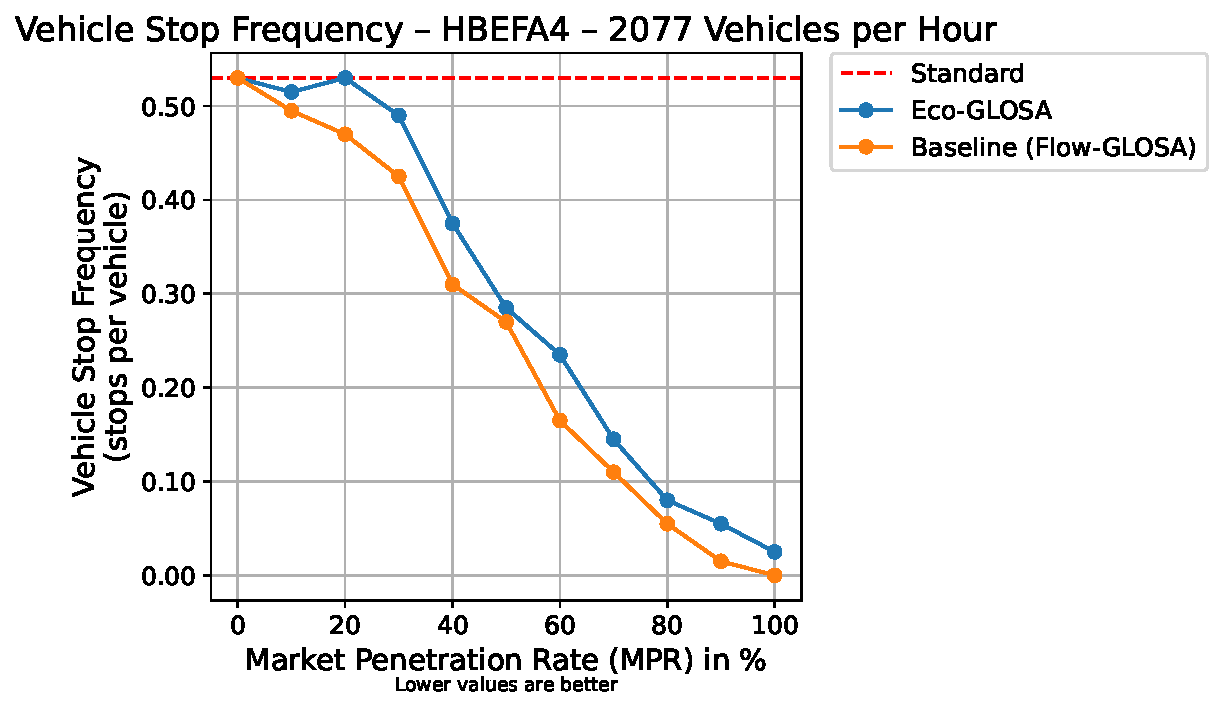
\includegraphics[width=\textwidth]{data/img/VehicleStopFrequency/VehicleStopFrequency_HBEFA4_Cars2077.pdf}
    \caption{Results under the HBEFA4 emission model.}
    \label{fig:StopFreq_2077_HBEFA4}
  \end{subfigure}
  \begin{subfigure}[b]{0.98\textwidth}
    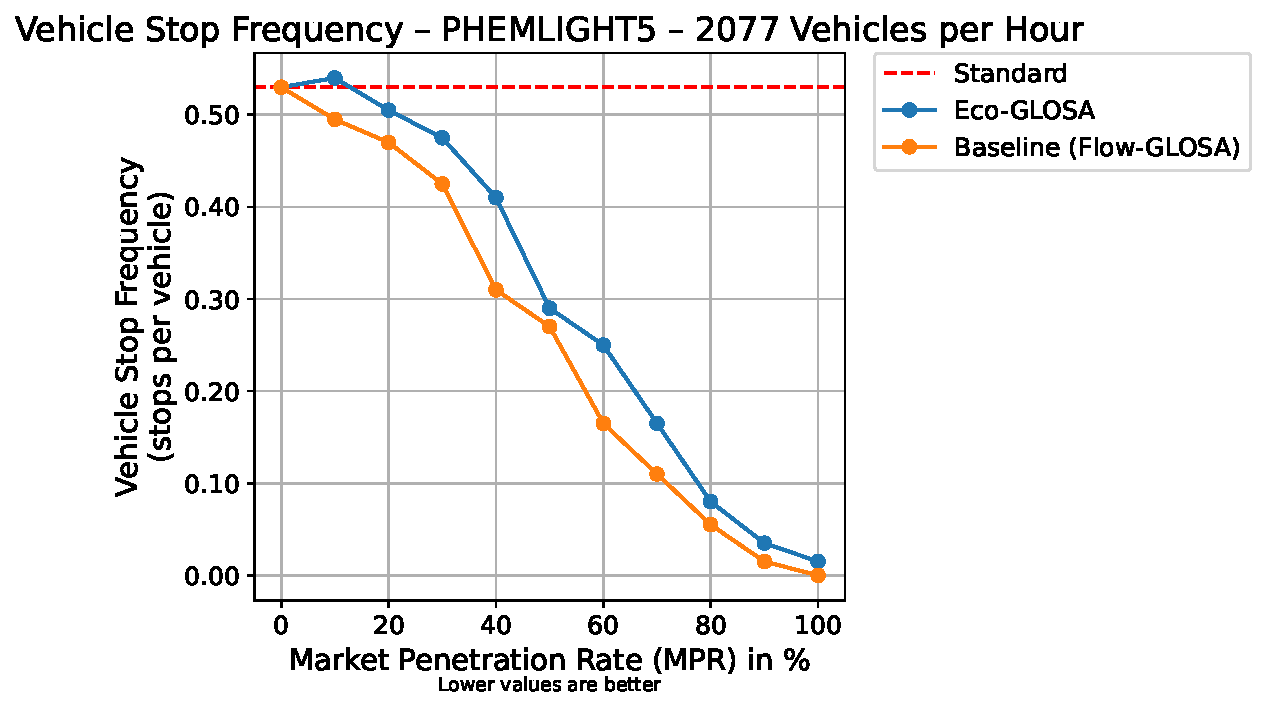
\includegraphics[width=\textwidth]{data/img/VehicleStopFrequency/VehicleStopFrequency_PHEMLIGHT5_Cars2077.pdf}
    \caption{Results under the PHEMlight5 emission model.}
    \label{fig:StopFreq_2077_PHEM}
  \end{subfigure}
  \caption[Vehicle stop frequency vs. \ac{mpr} at $2077~\unit{\veh\per\hour}$]{Vehicle stop frequency versus \ac{mpr} at an incipient congestion level of $2077~\unit{\veh\per\hour}$. The plots compare the Standard, \ac{eco-glosa}, and \ac{flow-glosa} controllers.}
  \label{fig:StopFreq_2077}
\end{figure}

\paragraph{High Demand ($2769~\unit{\veh\per\hour}$).}
This demand level reveals a critical performance divergence (Figure~\vref{fig:StopFreq_2769}). The \ac{flow-glosa} controller remains robust, maintaining a low stop frequency that declines smoothly as \ac{mpr} increases. In contrast, \ac{eco-glosa} becomes highly unstable. Under the PHEMlight5 model, its stop frequency increases sharply from the Standard value of $0.68~\unit{\stops\per\veh}$ to over $11.5~\unit{\stops\per\veh}$ at $90\%$ \ac{mpr}. The HBEFA4 model exhibits different volatility, with stop frequency oscillating and peaking at $8.02~\unit{\stops\per\veh}$ at $60\%$ \ac{mpr}. This behaviour highlights the risk of \ac{eco-glosa} actively inducing stop-and-go waves at the verge of congestion.

\begin{figure}[htbp]
  \centering
  \begin{subfigure}[b]{0.98\textwidth}
    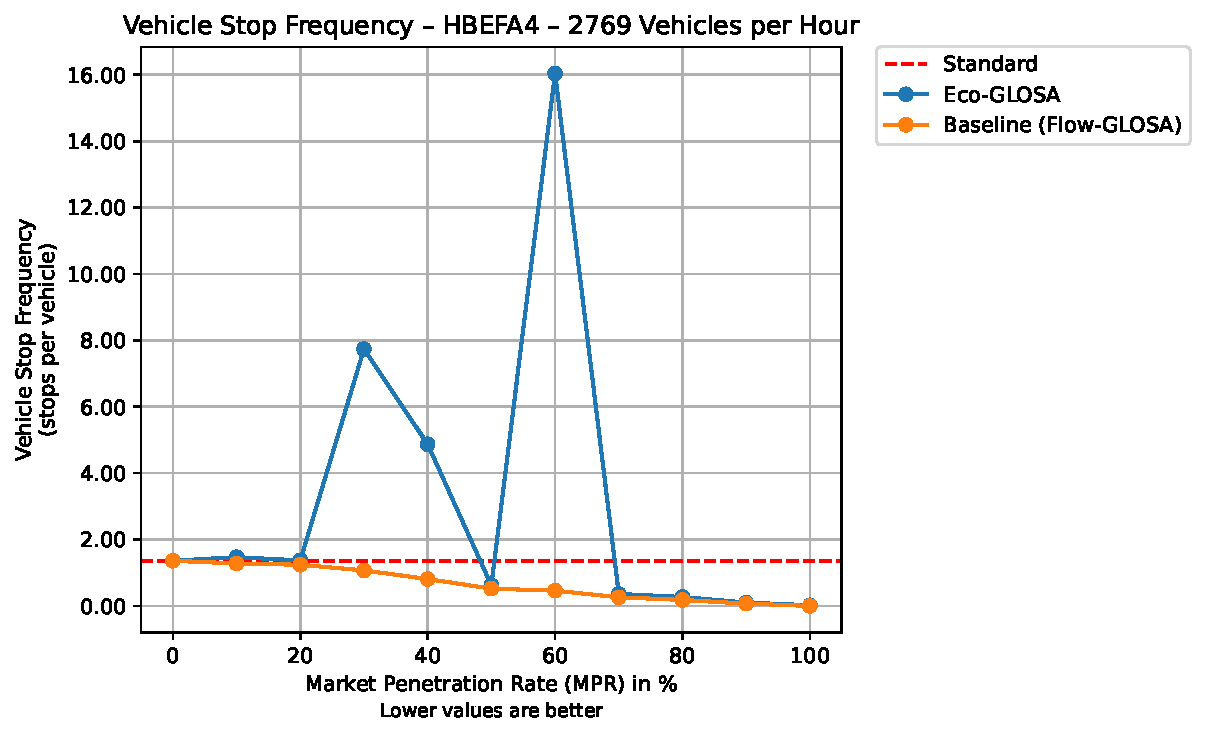
\includegraphics[width=\textwidth]{data/img/VehicleStopFrequency/VehicleStopFrequency_HBEFA4_Cars2769.pdf}
    \caption{Performance with the HBEFA4 emission model.}
    \label{fig:StopFreq_2769_HBEFA4}
  \end{subfigure}
  \begin{subfigure}[b]{0.98\textwidth}
    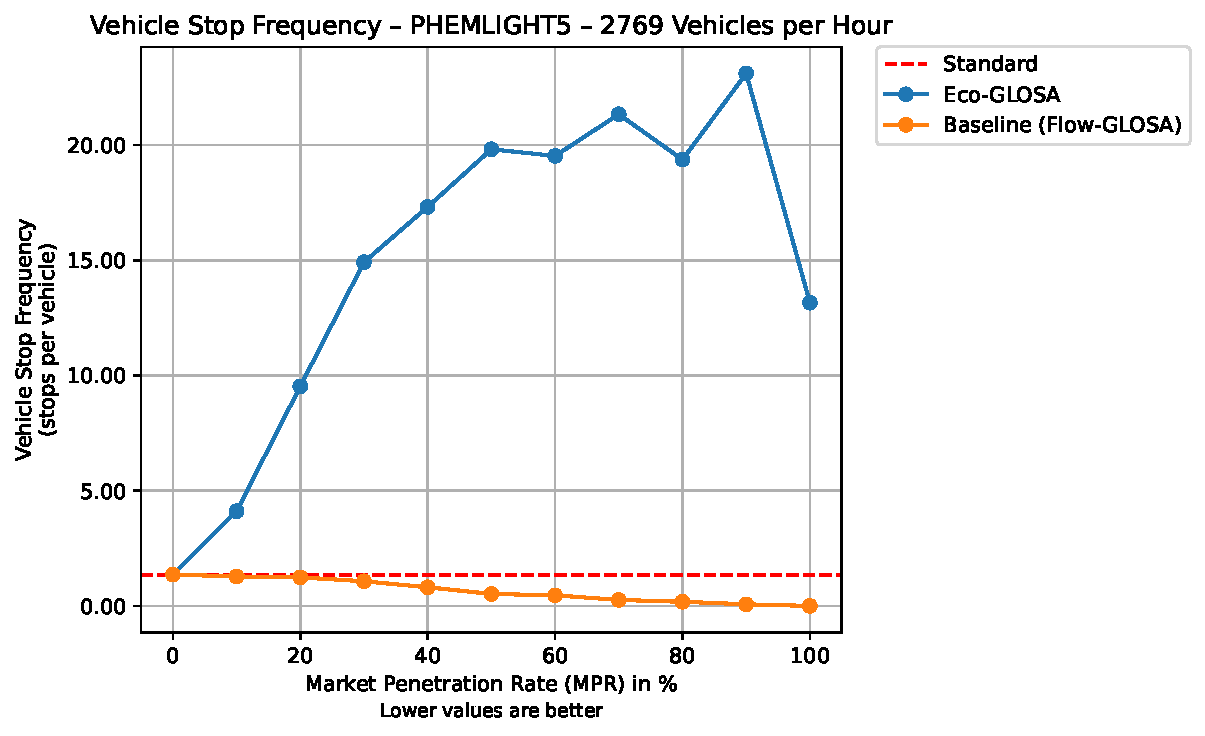
\includegraphics[width=\textwidth]{data/img/VehicleStopFrequency/VehicleStopFrequency_PHEMLIGHT5_Cars2769.pdf}
    \caption{Performance with the PHEMlight5 emission model.}
    \label{fig:StopFreq_2769_PHEM}
  \end{subfigure}
  \caption[Vehicle stop frequency vs. \ac{mpr} at $2769~\unit{\veh\per\hour}$]{Vehicle stop frequency versus \ac{mpr} at the jam threshold of $2769~\unit{\veh\per\hour}$. The plots illustrate the significant performance divergence of the two control strategies.}
  \label{fig:StopFreq_2769}
\end{figure}

\paragraph{Saturated Regime ($3462~\unit{\veh\per\hour}$).}
In the fully saturated regime, the Standard scenario is already gridlocked with a high stop frequency of $9.42~\unit{\stops\per\veh}$ (Figure~\vref{fig:StopFreq_3462}). Under these conditions, the \ac{eco-glosa} controller fails to improve conditions and instead exacerbates congestion, with its stop frequency increasing to over $17~\unit{\stops\per\veh}$ (HBEFA4) and $19~\unit{\stops\per\veh}$ (PHEMlight5). In the opposite direction, the \ac{flow-glosa} controller demonstrates a remarkable ability to prevent gridlock. Its effectiveness becomes apparent as penetration increases, with the stop frequency dropping sharply beyond $50\%$ \ac{mpr}. At full penetration, stops are reduced to near-zero levels ($0.005~\unit{\stops\per\veh}$). This profound reduction, supported by the sustained high average speeds shown in Figure~\vref{fig:MeanSpeed_3462}, confirms that a flow-optimised strategy successfully maintains free-flow conditions and prevents the onset of severe traffic jams even under saturated demand.

\begin{figure}[htbp]
  \centering
  \begin{subfigure}[b]{0.98\textwidth}
    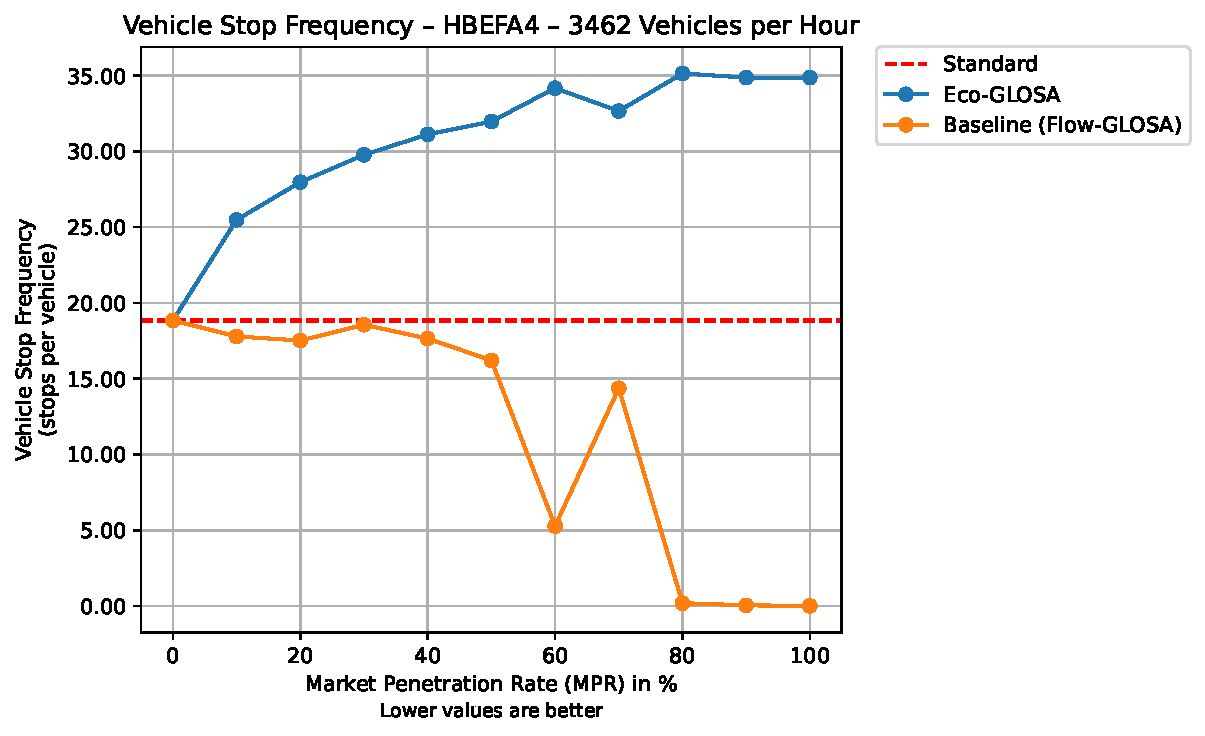
\includegraphics[width=\textwidth]{data/img/VehicleStopFrequency/VehicleStopFrequency_HBEFA4_Cars3462.pdf}
    \caption{Simulation results using the HBEFA4 model.}
    \label{fig:StopFreq_3462_HBEFA4}
  \end{subfigure}
  \begin{subfigure}[b]{0.98\textwidth}
    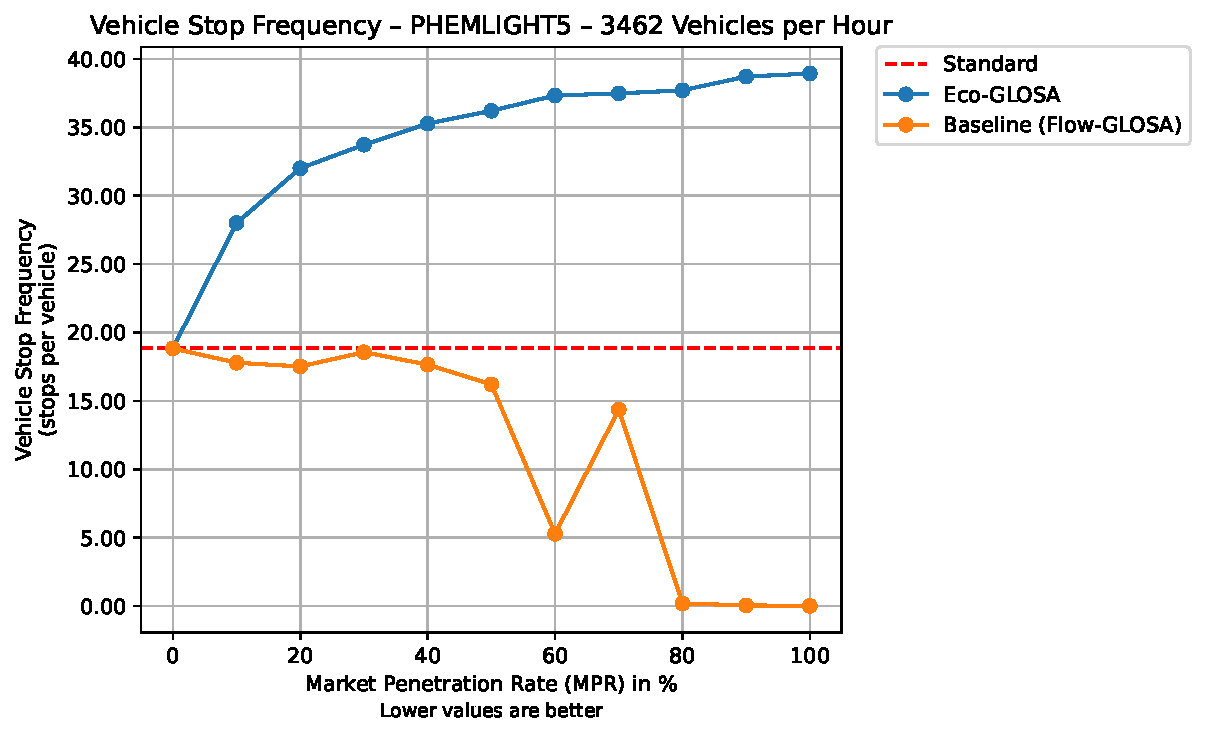
\includegraphics[width=\textwidth]{data/img/VehicleStopFrequency/VehicleStopFrequency_PHEMLIGHT5_Cars3462.pdf}
    \caption{Simulation results using the PHEMlight5 model.}
    \label{fig:StopFreq_3462_PHEM}
  \end{subfigure}
  \caption[Vehicle stop frequency vs. \ac{mpr} at $3462~\unit{\veh\per\hour}$]{Vehicle stop frequency as a function of \ac{mpr} in the fully saturated regime of $3462~\unit{\veh\per\hour}$. The outcomes for the Standard, \ac{eco-glosa}, and \ac{flow-glosa} controllers are shown.}
  \label{fig:StopFreq_3462}
\end{figure}

\paragraph{Implications.}
The stop frequency results reveal a significant performance inversion for the \ac{eco-glosa} controller. While it is highly effective at reducing stops in low to moderate demand, its behaviour becomes inconsistent and counterproductive as the system approaches capacity, actively increasing stops and inducing traffic instability. This creates a substantial operational risk, where a controller intended to improve efficiency instead causes network instability. The choice of emission model further complicates its performance, with the transient-sensitive PHEMlight5 model consistently triggering this failure at lower penetration rates than HBEFA4. Conversely, the \ac{flow-glosa} algorithm proves to be a robust strategy across all demand scenarios. Its consistent ability to suppress and prevent vehicle stops, particularly under high and saturated demand, underscores its value not just for optimising flow but for ensuring network stability.

\paragraph{Key Takeaways.}
\begin{enumerate}
    \item \textbf{Low Demand Performance:} In light to moderate demand scenarios ($69$--$1385~\unit{\veh\per\hour}$), both \ac{eco-glosa} and \ac{flow-glosa} are highly effective, significantly reducing vehicle stop frequency as their market penetration increases.
    \item \textbf{Performance Inversion:} \ac{eco-glosa} exhibits a critical performance inversion. Its benefits in low-demand scenarios are reversed at high demands ($ \geq 2769~\unit{\veh\per\hour}$), where it becomes unstable and significantly increases stop frequency compared to the uncontrolled Standard.
    \item \textbf{Robustness of \ac{flow-glosa}:} The \ac{flow-glosa} controller is robust across all tested demand levels, consistently maintaining or reducing stop frequency.
    \item \textbf{Gridlock Prevention:} In fully saturated conditions ($3462~\unit{\veh\per\hour}$), where the Standard scenario is gridlocked, \ac{flow-glosa} is capable of preventing this breakdown. At high penetration rates, it drives stop counts to near-zero, thereby maintaining free-flow conditions.
\end{enumerate}

\begin{table}[htb]
  \centering
  \caption[Vehicle stop frequency for all traffic volumes and \ac{mpr} values]{Vehicle stop frequency, measured in $\unit{\stops\per\veh}$, tabulated for all traffic volumes and \ac{mpr} values. Data is provided for the Standard, \ac{flow-glosa}, and \ac{eco-glosa} controllers under both the HBEFA4 and PHEMlight5 emission models.}
  \label{tab:StopFreq}
  \resizebox{\textwidth}{!}{%
  \begin{tabular}{r l l r *{10}{r}}
    \toprule
    Vehicles & Algorithm & Fuel Model & \textbf{0\% (Standard)} & 10\% & 20\% & 30\% & 40\% & 50\% & 60\% & 70\% & 80\% & 90\% & 100\%\\
    \midrule
    69  & \ac{eco-glosa} & HBEFA4 & \textbf{0.38} & 0.28 & 0.36 & 0.28 & 0.245 & 0.27 & 0.215 & 0.11 & 0.14 & 0.055 & 0\\
    69  & Baseline (\ac{flow-glosa}) & HBEFA4 & \textbf{0.38} & 0.28 & 0.39 & 0.305 & 0.245 & 0.27 & 0.245 & 0.11 & 0.14 & 0.085 & 0\\
    69  & \ac{eco-glosa} & PHEMLIGHT5 & \textbf{0.38} & 0.28 & 0.36 & 0.25 & 0.245 & 0.27 & 0.215 & 0.11 & 0.14 & 0.055 & 0\\
    69  & Baseline (\ac{flow-glosa}) & PHEMLIGHT5 & \textbf{0.38} & 0.28 & 0.39 & 0.305 & 0.245 & 0.27 & 0.245 & 0.11 & 0.14 & 0.085 & 0\\
    \midrule
    138 & \ac{eco-glosa} & HBEFA4 & \textbf{0.415} & 0.32 & 0.32 & 0.295 & 0.185 & 0.135 & 0.135 & 0.095 & 0.065 & 0.04 & 0\\
    138 & Baseline (\ac{flow-glosa}) & HBEFA4 & \textbf{0.415} & 0.305 & 0.31 & 0.295 & 0.185 & 0.16 & 0.12 & 0.08 & 0.08 & 0.025 & 0\\
    138 & \ac{eco-glosa} & PHEMLIGHT5 & \textbf{0.415} & 0.335 & 0.28 & 0.295 & 0.185 & 0.145 & 0.08 & 0.095 & 0.065 & 0.04 & 0\\
    138 & Baseline (\ac{flow-glosa}) & PHEMLIGHT5 & \textbf{0.415} & 0.305 & 0.31 & 0.295 & 0.185 & 0.16 & 0.12 & 0.08 & 0.08 & 0.025 & 0\\
    \midrule
    346 & \ac{eco-glosa} & HBEFA4 & \textbf{0.38} & 0.34 & 0.325 & 0.255 & 0.235 & 0.19 & 0.14 & 0.135 & 0.095 & 0.04 & 0.005\\
    346 & Baseline (\ac{flow-glosa}) & HBEFA4 & \textbf{0.38} & 0.345 & 0.32 & 0.245 & 0.22 & 0.18 & 0.12 & 0.135 & 0.075 & 0.03 & 0\\
    346 & \ac{eco-glosa} & PHEMLIGHT5 & \textbf{0.38} & 0.325 & 0.365 & 0.28 & 0.255 & 0.175 & 0.155 & 0.135 & 0.085 & 0.035 & 0.015\\
    346 & Baseline (\ac{flow-glosa}) & PHEMLIGHT5 & \textbf{0.38} & 0.345 & 0.32 & 0.245 & 0.22 & 0.18 & 0.12 & 0.135 & 0.075 & 0.03 & 0\\
    \midrule
    692 & \ac{eco-glosa} & HBEFA4 & \textbf{0.395} & 0.39 & 0.31 & 0.27 & 0.225 & 0.21 & 0.115 & 0.13 & 0.08 & 0.03 & 0.005\\
    692 & Baseline (\ac{flow-glosa}) & HBEFA4 & \textbf{0.395} & 0.35 & 0.315 & 0.265 & 0.225 & 0.185 & 0.115 & 0.11 & 0.065 & 0.025 & 0.005\\
    692 & \ac{eco-glosa} & PHEMLIGHT5 & \textbf{0.395} & 0.345 & 0.33 & 0.3 & 0.25 & 0.205 & 0.145 & 0.125 & 0.1 & 0.025 & 0.005\\
    692 & Baseline (\ac{flow-glosa}) & PHEMLIGHT5 & \textbf{0.395} & 0.35 & 0.315 & 0.265 & 0.225 & 0.185 & 0.115 & 0.11 & 0.065 & 0.025 & 0.005\\
    \midrule
    1385 & \ac{eco-glosa} & HBEFA4 & \textbf{0.455} & 0.45 & 0.41 & 0.345 & 0.29 & 0.23 & 0.205 & 0.125 & 0.095 & 0.05 & 0.01\\
    1385 & Baseline (\ac{flow-glosa}) & HBEFA4 & \textbf{0.455} & 0.42 & 0.395 & 0.35 & 0.275 & 0.2 & 0.155 & 0.105 & 0.065 & 0.04 & 0\\
    1385 & \ac{eco-glosa} & PHEMLIGHT5 & \textbf{0.455} & 0.445 & 0.405 & 0.375 & 0.285 & 0.215 & 0.215 & 0.11 & 0.11 & 0.045 & 0.025\\
    1385 & Baseline (\ac{flow-glosa}) & PHEMLIGHT5 & \textbf{0.455} & 0.42 & 0.395 & 0.35 & 0.275 & 0.2 & 0.155 & 0.105 & 0.065 & 0.04 & 0\\
    \midrule
    2077 & \ac{eco-glosa} & HBEFA4 & \textbf{0.53} & 0.515 & 0.53 & 0.49 & 0.375 & 0.285 & 0.235 & 0.145 & 0.08 & 0.055 & 0.025\\
    2077 & Baseline (\ac{flow-glosa}) & HBEFA4 & \textbf{0.53} & 0.495 & 0.47 & 0.425 & 0.31 & 0.27 & 0.165 & 0.11 & 0.055 & 0.015 & 0\\
    2077 & \ac{eco-glosa} & PHEMLIGHT5 & \textbf{0.53} & 0.54 & 0.505 & 0.475 & 0.41 & 0.29 & 0.25 & 0.165 & 0.08 & 0.035 & 0.015\\
    2077 & Baseline (\ac{flow-glosa}) & PHEMLIGHT5 & \textbf{0.53} & 0.495 & 0.47 & 0.425 & 0.31 & 0.27 & 0.165 & 0.11 & 0.055 & 0.015 & 0\\
    \midrule
    \textbf{2769} & \textbf{\ac{eco-glosa}} & \textbf{HBEFA4} & \textbf{0.68} & \textbf{0.735} & \textbf{0.685} & \textbf{3.87} & \textbf{2.435} & \textbf{0.31} & \textbf{8.02} & \textbf{0.18} & \textbf{0.135} & \textbf{0.05} & \textbf{0.01}\\
    2769 & Baseline (\ac{flow-glosa}) & HBEFA4 & \textbf{0.68} & 0.64 & 0.62 & 0.535 & 0.405 & 0.26 & 0.23 & 0.13 & 0.09 & 0.035 & 0\\
    \textbf{2769} & \textbf{\ac{eco-glosa}} & \textbf{PHEMLIGHT5} & \textbf{0.68} & \textbf{2.055} & \textbf{4.765} & \textbf{7.46} & \textbf{8.66} & \textbf{9.91} & \textbf{9.765} & \textbf{10.67} & \textbf{9.685} & \textbf{11.555} & \textbf{6.58}\\
    2769 & Baseline (\ac{flow-glosa}) & PHEMLIGHT5 & \textbf{0.68} & 0.64 & 0.62 & 0.535 & 0.405 & 0.26 & 0.23 & 0.13 & 0.09 & 0.035 & 0\\
    \midrule
    \textbf{3462} & \textbf{\ac{eco-glosa}} & \textbf{HBEFA4} & \textbf{9.42} & \textbf{12.74} & \textbf{13.985} & \textbf{14.885} & \textbf{15.56} & \textbf{15.985} & \textbf{17.085} & \textbf{16.33} & \textbf{17.57} & \textbf{17.435} & \textbf{17.435}\\
    3462 & Baseline (\ac{flow-glosa}) & HBEFA4 & \textbf{9.42} & 8.895 & 8.76 & 9.28 & 8.825 & 8.105 & 2.64 & 7.185 & \textbf{0.095} & \textbf{0.025} & \textbf{0.005}\\
    \textbf{3462} & \textbf{\ac{eco-glosa}} & \textbf{PHEMLIGHT5} & \textbf{9.42} & \textbf{14.005} & \textbf{16.005} & \textbf{16.865} & \textbf{17.635} & \textbf{18.105} & \textbf{18.665} & \textbf{18.74} & \textbf{18.855} & \textbf{19.355} & \textbf{19.47}\\
    3462 & Baseline (\ac{flow-glosa}) & PHEMLIGHT5 & \textbf{9.42} & 8.895 & 8.76 & 9.28 & 8.825 & 8.105 & 2.64 & 7.185 & \textbf{0.095} & \textbf{0.025} & \textbf{0.005}\\
    \bottomrule
  \end{tabular}}
\end{table}

\section{Driving Smoothness}
\label{sec:Results_Smoothness}

The analysis of driving smoothness examines the average acceleration, $\gls{a}$, and average jerk, $\gls{j}$, as functions of the \ac{mpr}. Table~\vref{tab:DrivingSmoothness} reports the paired values $(\gls{a}, \gls{j})$ for the Standard, \ac{flow-glosa}, and \ac{eco-glosa} configurations under both emission models. Figures~\vref{fig:Smoothness_692}, \vref{fig:Smoothness_2769}, and \vref{fig:Smoothness_3462} illustrate these trends at representative traffic volumes.

\paragraph{\ac{eco-glosa} at Low to Medium Volumes}
Under the \ac{eco-glosa} controller, an inverse relationship between average acceleration and jerk emerges as \ac{mpr} increases. At a demand of $69~\unit{\veh\per\hour}$ with the HBEFA4 model, acceleration falls from $0.30~\unit{\metre\per\second\squared}$ to $0.25~\unit{\metre\per\second\squared}$ (a $17\%$ reduction), while jerk rises from $0.74~\unit{\metre\per\second\cubed}$ to $0.81~\unit{\metre\per\second\cubed}$ (a $9\%$ increase). This pattern, where gentler accelerations are offset by sharper adjustments, is consistent across the PHEMlight5 model and persists at higher moderate volumes such as $692~\unit{\veh\per\hour}$, as seen in Figure~\vref{fig:Smoothness_692}.

\begin{figure}[htb]
  \centering
  \begin{subfigure}[b]{0.45\textwidth}
    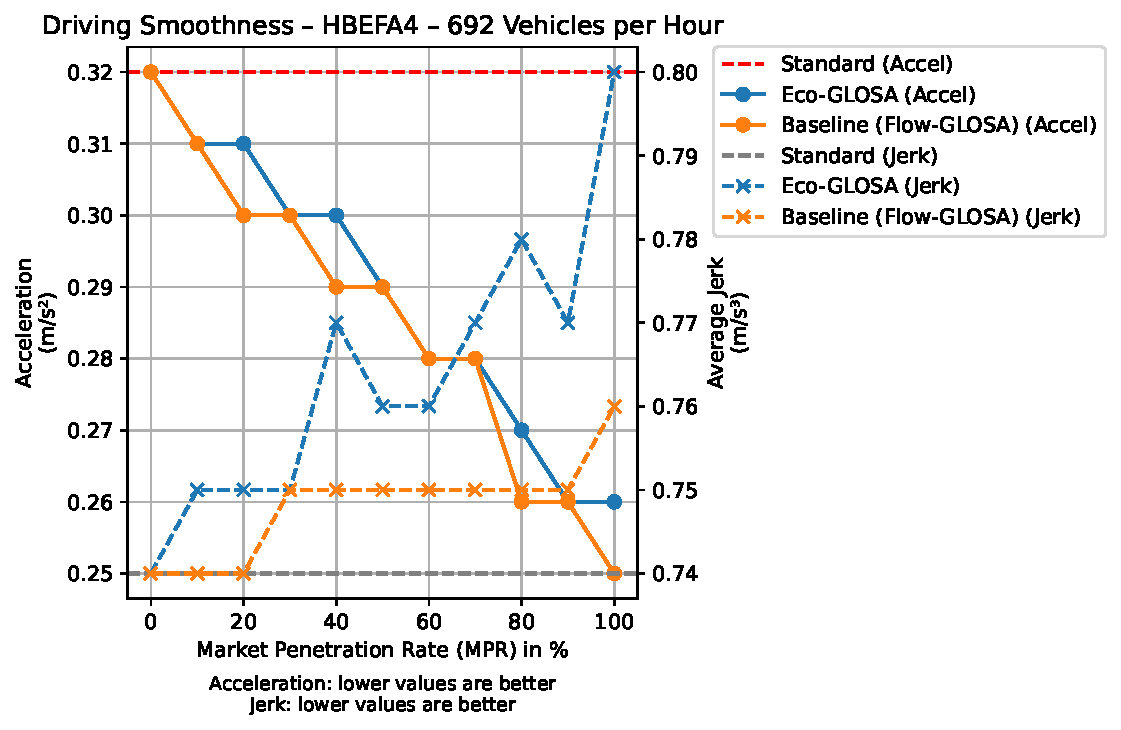
\includegraphics[width=\textwidth]{data/img/DrivingSmoothness/DrivingSmoothness_HBEFA4_Cars692.pdf}
    \caption{Results under the HBEFA4 emission model.}
    \label{fig:Smoothness_HBEFA4_692}
  \end{subfigure}\hfill
  \begin{subfigure}[b]{0.45\textwidth}
    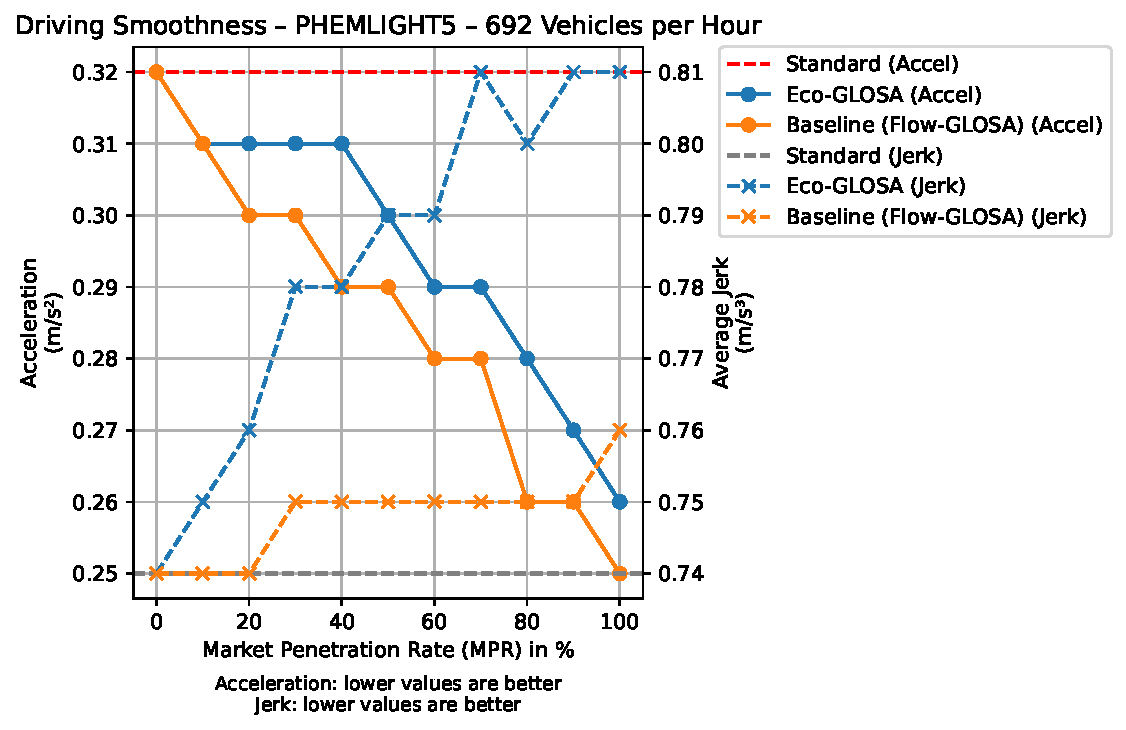
\includegraphics[width=\textwidth]{data/img/DrivingSmoothness/DrivingSmoothness_PHEMLIGHT5_Cars692.pdf}
    \caption{Results under the PHEMlight5 emission model.}
    \label{fig:Smoothness_PHEMlight5_692}
  \end{subfigure}
  \caption[Driving smoothness metrics at $692~\unit{\veh\per\hour}$]{Driving smoothness metrics at a moderate demand of $692~\unit{\veh\per\hour}$. The plots compare average acceleration and jerk for the Standard, \ac{eco-glosa}, and \ac{flow-glosa} controllers.}
  \label{fig:Smoothness_692}
\end{figure}

\paragraph{\ac{eco-glosa} at High Volume ($2769~\unit{\veh\per\hour}$).}
At this demand level, the HBEFA4 model shows fluctuating acceleration values under \ac{eco-glosa}, which rise from the Standard $0.36~\unit{\metre\per\second\squared}$ to $0.41~\unit{\metre\per\second\squared}$ before gradually declining. With the PHEMlight5 model, however, the outcome is more favourable; while not monotonic, the acceleration improves from $0.36~\unit{\metre\per\second\squared}$ to $0.33~\unit{\metre\per\second\squared}$ at full penetration. More significantly, jerk declines to $0.66~\unit{\metre\per\second\cubed}$, a value $13\%$ below the Standard of $0.76~\unit{\metre\per\second\cubed}$ (Figure~\vref{fig:Smoothness_PHEMlight5_2769}). The persistently lower jerk at high \ac{mpr} suggests that once vehicles navigate the initial jam, they maintain smoother trajectories.

\begin{figure}[htb]
  \centering
  \begin{subfigure}[b]{0.45\textwidth}
    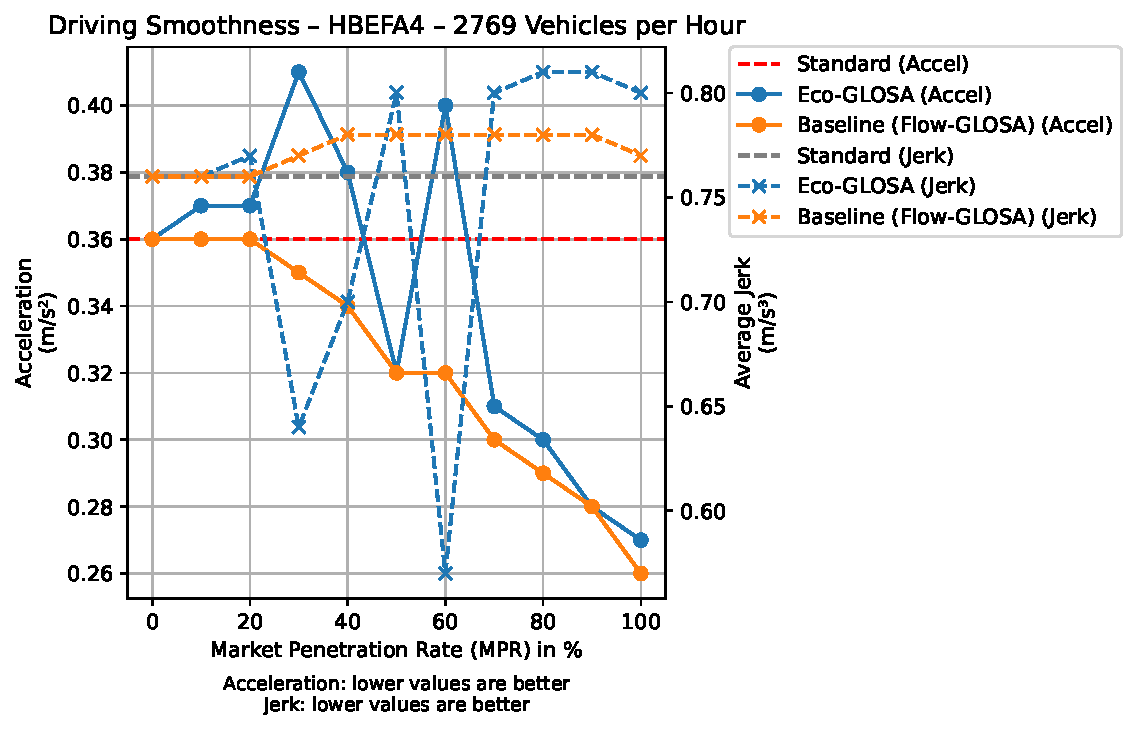
\includegraphics[width=\textwidth]{data/img/DrivingSmoothness/DrivingSmoothness_HBEFA4_Cars2769.pdf}
    \caption{Performance with the HBEFA4 emission model.}
    \label{fig:Smoothness_HBEFA4_2769}
  \end{subfigure}\hfill
  \begin{subfigure}[b]{0.45\textwidth}
    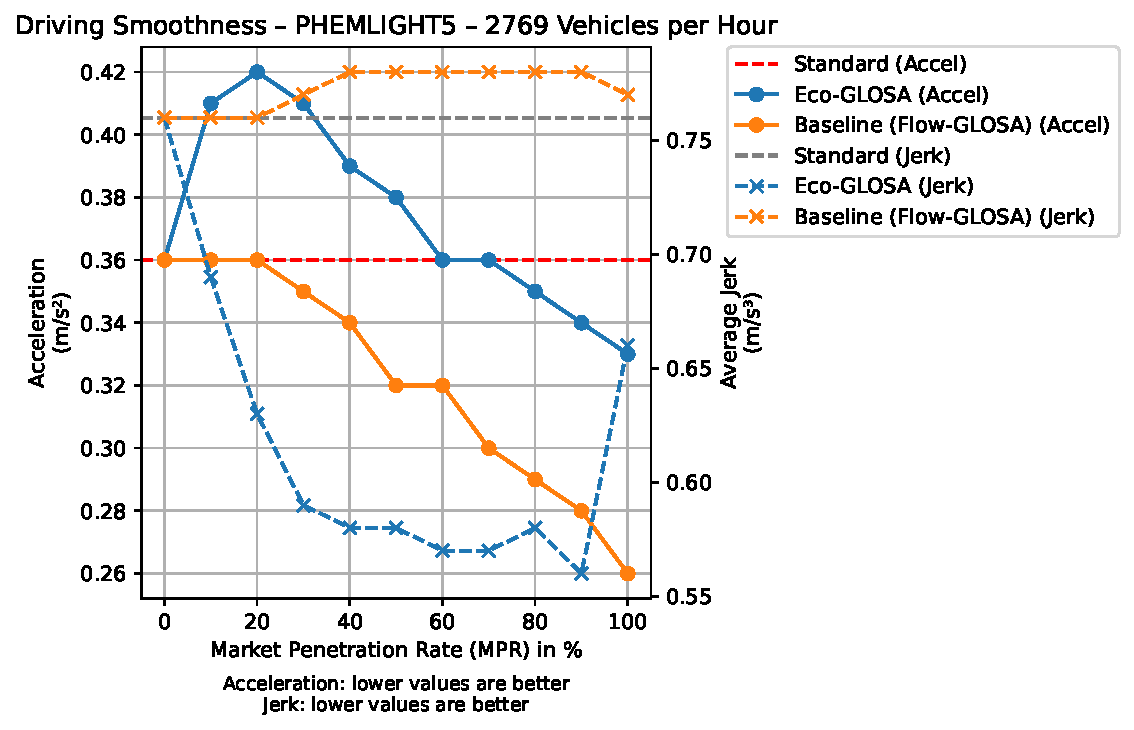
\includegraphics[width=\textwidth]{data/img/DrivingSmoothness/DrivingSmoothness_PHEMLIGHT5_Cars2769.pdf}
    \caption{Performance with the PHEMlight5 emission model.}
    \label{fig:Smoothness_PHEMlight5_2769}
  \end{subfigure}
  \caption[Driving smoothness vs. \ac{mpr} at $2769~\unit{\veh\per\hour}$]{Driving smoothness as a function of \ac{mpr} at the jam threshold of $2769~\unit{\veh\per\hour}$. The plots show the performance of the three controller strategies under two emission models.}
  \label{fig:Smoothness_2769}
\end{figure}

\paragraph{\ac{eco-glosa} at Full Saturation ($3462~\unit{\veh\per\hour}$).}
In the fully saturated regime, both models show clear improvements in smoothness as \ac{mpr} increases. For HBEFA4, acceleration decreases from $0.55$ to $0.38~\unit{\metre\per\second\squared}$ ($31\%$ reduction), and jerk from $0.57$ to $0.51~\unit{\metre\per\second\cubed}$ ($11\%$ reduction) at $100\%$ \ac{mpr}. The PHEMlight5 model shows comparable gains, with acceleration falling to $0.35~\unit{\metre\per\second\squared}$ and jerk to $0.52~\unit{\metre\per\second\cubed}$. However, these smoothness improvements must be interpreted within the context of the traffic jam. As established in Sections~\vref{sec:Results_MeanSpeed} and \vref{sec:Results_Stops}, the controller fails to increase the low average speed or reduce the high stop frequency. Therefore, the data does not indicate a dissolution of the jam. Instead, it suggests that the controller successfully modifies the \enquote{character} of the stop-and-go waves. The aggressive, high-acceleration manoeuvres typical of a congested state are replaced by a smoother, less frantic \enquote{creeping} behaviour. While this change enhances ride comfort, the persistent gridlock confirms that the \ac{eco-glosa} strategy cannot overcome the fundamental capacity limitations at this extreme demand level.

\begin{figure}[htb]
  \centering
  \begin{subfigure}[b]{0.45\textwidth}
    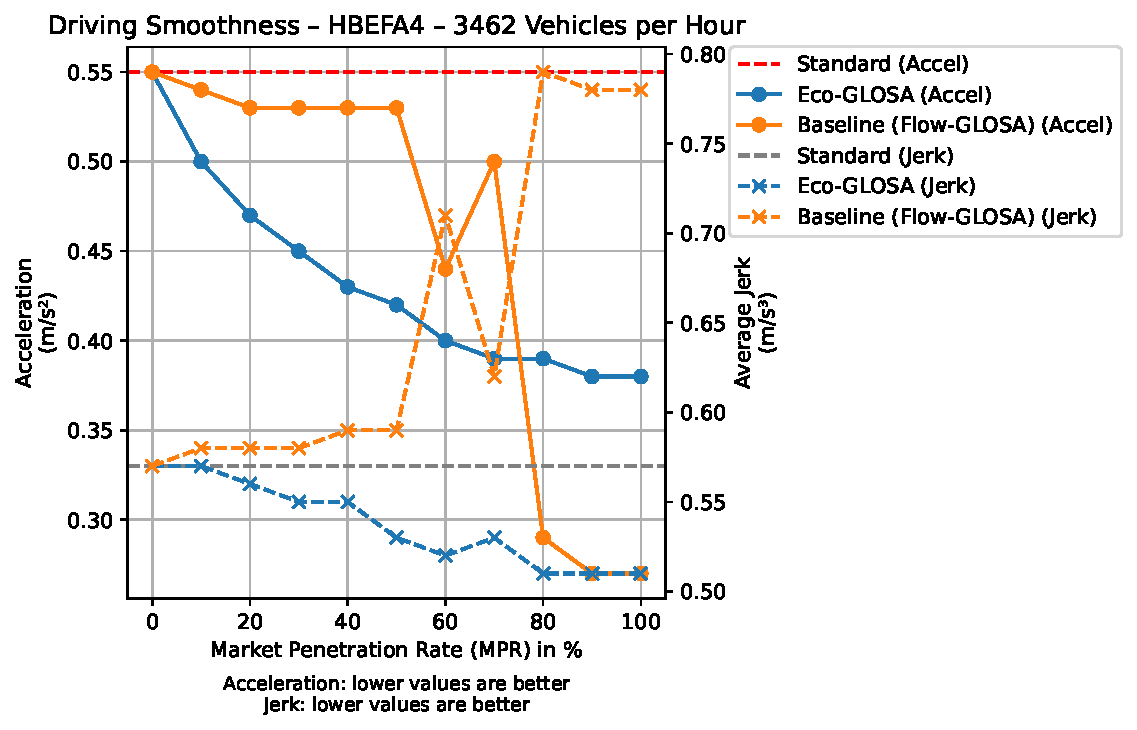
\includegraphics[width=\textwidth]{data/img/DrivingSmoothness/DrivingSmoothness_HBEFA4_Cars3462.pdf}
    \caption{Simulation results using the HBEFA4 model.}
    \label{fig:Smoothness_HBEFA4_3462}
  \end{subfigure}\hfill
  \begin{subfigure}[b]{0.45\textwidth}
    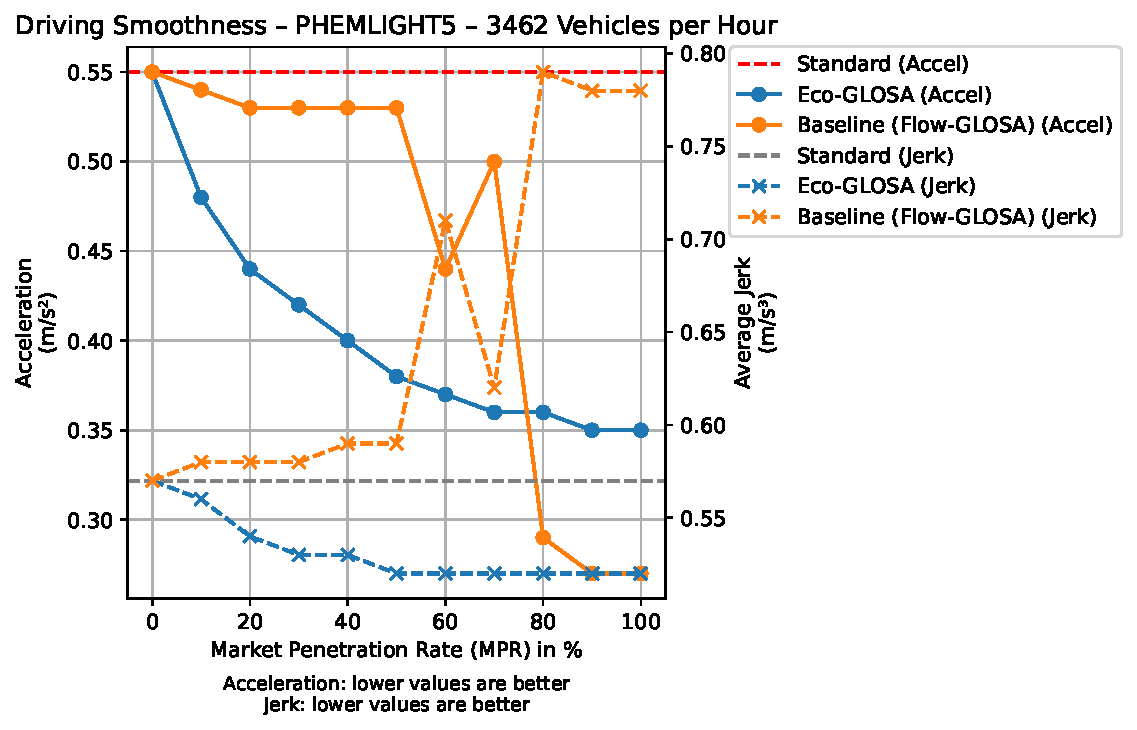
\includegraphics[width=\textwidth]{data/img/DrivingSmoothness/DrivingSmoothness_PHEMLIGHT5_Cars3462.pdf}
    \caption{Simulation results using the PHEMlight5 model.}
    \label{fig:Smoothness_PHEMlight5_3462}
  \end{subfigure}
  \caption[Driving smoothness metrics at $3462~\unit{\veh\per\hour}$]{Driving smoothness metrics in the fully saturated regime ($3462~\unit{\veh\per\hour}$). The plots compare the Standard, \ac{eco-glosa}, and \ac{flow-glosa} controllers.}
  \label{fig:Smoothness_3462}
\end{figure}

\paragraph{\ac{flow-glosa} Comparison.}
The \ac{flow-glosa} controller offers acceleration improvements comparable to \ac{eco-glosa} but generally maintains a more stable and consistently lower jerk profile, except in specific high-saturation scenarios. At low to medium volumes, its application reduces average acceleration by approximately $15\%$ to $20\%$ from the Standard, with only a minimal corresponding increase in average jerk.
\mynewline
The controller's dynamics shift significantly under full saturation ($3462~\unit{\veh\per\hour}$). It exhibits a notable jerk spike from $0.59~\unit{\metre\per\second\cubed}$ to $0.71~\unit{\metre\per\second\cubed}$ at an \ac{mpr} of $60\%$. This transient corresponds precisely to the point where the traffic jam dissolves and vehicles begin to resume free-flow speeds. A second, more pronounced peak appears at $80\%$ \ac{mpr}, which does not stem from an incoming jam but rather from platoon-based micro-adjustments. With such a high share of equipped vehicles, tight clusters form and must continually react to signal timings. Minor mismatches can force abrupt, platoon-wide decelerations and subsequent re-accelerations, which drives the observed increase in average jerk.

\begin{table}[htb]
  \centering
  \caption[Average acceleration and jerk across all volumes and \acp{mpr}]{Driving smoothness, detailed by average acceleration ($\unit{\metre\per\second\squared}$) and jerk ($\unit{\metre\per\second\cubed}$), across all traffic volumes and \acp{mpr}. Results are provided for the Standard, \ac{flow-glosa}, and \ac{eco-glosa} configurations.}
  \label{tab:DrivingSmoothness}
  \resizebox{\textwidth}{!}{%
    \begin{tabular}{l l l *{11}{c}}
      \toprule
      Vehicles & Algorithm & Model       & \textbf{0\% (Standard)} & 10\%        & 20\%        & 30\%        & 40\%        & 50\%        & 60\%        & 70\%        & 80\%        & 90\%        & 100\%       \\
      \midrule
      \textbf{69.0}  & Eco-GLOSA                   & HBEFA4      & \textbf{0.3, 0.74}   & 0.29, 0.75  & 0.31, 0.76  & 0.28, 0.77  & 0.29, 0.77  & 0.29, 0.79  & 0.27, 0.77  & 0.25, 0.81  & 0.28, 0.80  & 0.24, 0.79  & 0.25, 0.81  \\
      \textbf{69.0}  & Baseline (Flow-GLOSA)       & HBEFA4      & \textbf{0.3, 0.74}   & 0.29, 0.76  & 0.31, 0.75  & 0.28, 0.75  & 0.28, 0.75  & 0.29, 0.75  & 0.28, 0.74  & 0.25, 0.75  & 0.27, 0.75  & 0.25, 0.75  & 0.25, 0.77  \\
      \textbf{69.0}  & Eco-GLOSA                   & PHEMlight5  & \textbf{0.3, 0.74}   & 0.29, 0.76  & 0.29, 0.75  & 0.28, 0.76  & 0.27, 0.78  & 0.28, 0.78  & 0.27, 0.80  & 0.25, 0.81  & 0.27, 0.80  & 0.24, 0.79  & 0.23, 0.81  \\
      \textbf{69.0}  & Baseline (Flow-GLOSA)       & PHEMlight5  & \textbf{0.3, 0.74}   & 0.29, 0.76  & 0.31, 0.75  & 0.28, 0.75  & 0.28, 0.75  & 0.29, 0.75  & 0.28, 0.74  & 0.25, 0.75  & 0.27, 0.75  & 0.25, 0.75  & 0.25, 0.77  \\
      \midrule
      \textbf{138.0} & Eco-GLOSA                   & HBEFA4      & \textbf{0.31, 0.73}  & 0.29, 0.74  & 0.30, 0.74  & 0.28, 0.74  & 0.28, 0.77  & 0.27, 0.76  & 0.28, 0.77  & 0.25, 0.77  & 0.27, 0.78  & 0.26, 0.79  & 0.25, 0.78  \\
      \textbf{138.0} & Baseline (Flow-GLOSA)       & HBEFA4      & \textbf{0.31, 0.73}  & 0.29, 0.74  & 0.30, 0.75  & 0.30, 0.73  & 0.28, 0.75  & 0.28, 0.74  & 0.27, 0.75  & 0.26, 0.74  & 0.27, 0.75  & 0.26, 0.74  & 0.25, 0.75  \\
      \textbf{138.0} & Eco-GLOSA                   & PHEMlight5  & \textbf{0.31, 0.73}  & 0.30, 0.73  & 0.29, 0.75  & 0.28, 0.75  & 0.28, 0.77  & 0.26, 0.76  & 0.26, 0.78  & 0.26, 0.77  & 0.26, 0.79  & 0.25, 0.79  & 0.24, 0.79  \\
      \textbf{138.0} & Baseline (Flow-GLOSA)       & PHEMlight5  & \textbf{0.31, 0.73}  & 0.29, 0.74  & 0.30, 0.75  & 0.30, 0.73  & 0.28, 0.75  & 0.28, 0.74  & 0.27, 0.75  & 0.26, 0.74  & 0.27, 0.75  & 0.26, 0.74  & 0.25, 0.75  \\
      \midrule
      \textbf{346.0} & Eco-GLOSA                   & HBEFA4      & \textbf{0.31, 0.74}  & 0.31, 0.75  & 0.31, 0.76  & 0.30, 0.76  & 0.29, 0.76  & 0.29, 0.77  & 0.28, 0.77  & 0.28, 0.77  & 0.27, 0.77  & 0.26, 0.79  & 0.25, 0.80  \\
      \textbf{346.0} & Baseline (Flow-GLOSA)       & HBEFA4      & \textbf{0.31, 0.74}  & 0.31, 0.76  & 0.30, 0.75  & 0.30, 0.76  & 0.29, 0.76  & 0.29, 0.76  & 0.27, 0.75  & 0.28, 0.75  & 0.26, 0.76  & 0.26, 0.76  & 0.24, 0.76  \\
      \textbf{346.0} & Eco-GLOSA                   & PHEMlight5  & \textbf{0.31, 0.74}  & 0.31, 0.75  & 0.31, 0.77  & 0.30, 0.77  & 0.29, 0.77  & 0.28, 0.80  & 0.28, 0.79  & 0.28, 0.78  & 0.26, 0.79  & 0.26, 0.80  & 0.25, 0.82  \\
      \textbf{346.0} & Baseline (Flow-GLOSA)       & PHEMlight5  & \textbf{0.31, 0.74}  & 0.31, 0.76  & 0.30, 0.75  & 0.30, 0.76  & 0.29, 0.76  & 0.29, 0.76  & 0.27, 0.75  & 0.28, 0.75  & 0.26, 0.76  & 0.26, 0.76  & 0.24, 0.76  \\
      \midrule
      \textbf{692.0} & Eco-GLOSA                   & HBEFA4      & \textbf{0.32, 0.74}  & 0.31, 0.75  & 0.31, 0.75  & 0.30, 0.75  & 0.30, 0.77  & 0.29, 0.76  & 0.28, 0.76  & 0.28, 0.77  & 0.27, 0.78  & 0.26, 0.77  & 0.26, 0.80  \\
      \textbf{692.0} & Baseline (Flow-GLOSA)       & HBEFA4      & \textbf{0.32, 0.74}  & 0.31, 0.74  & 0.30, 0.74  & 0.30, 0.75  & 0.29, 0.75  & 0.29, 0.75  & 0.28, 0.75  & 0.28, 0.75  & 0.26, 0.75  & 0.26, 0.75  & 0.25, 0.76  \\
      \textbf{692.0} & Eco-GLOSA                   & PHEMlight5  & \textbf{0.32, 0.74}  & 0.31, 0.75  & 0.31, 0.76  & 0.31, 0.78  & 0.31, 0.78  & 0.30, 0.79  & 0.29, 0.79  & 0.29, 0.81  & 0.28, 0.80  & 0.27, 0.81  & 0.26, 0.81  \\
      \textbf{692.0} & Baseline (Flow-GLOSA)       & PHEMlight5  & \textbf{0.32, 0.74}  & 0.31, 0.74  & 0.30, 0.74  & 0.30, 0.75  & 0.29, 0.75  & 0.29, 0.75  & 0.28, 0.75  & 0.28, 0.75  & 0.26, 0.75  & 0.26, 0.75  & 0.25, 0.76  \\
      \midrule
      \textbf{1385.0}& Eco-GLOSA                   & HBEFA4      & \textbf{0.33, 0.74}  & 0.33, 0.75  & 0.33, 0.76  & 0.32, 0.77  & 0.31, 0.77  & 0.31, 0.77  & 0.30, 0.78  & 0.29, 0.78  & 0.28, 0.78  & 0.27, 0.78  & 0.26, 0.78  \\
      \textbf{1385.0}& Baseline (Flow-GLOSA)       & HBEFA4      & \textbf{0.33, 0.74}  & 0.33, 0.75  & 0.33, 0.75  & 0.32, 0.76  & 0.31, 0.76  & 0.30, 0.76  & 0.29, 0.76  & 0.29, 0.76  & 0.27, 0.76  & 0.27, 0.76  & 0.26, 0.75  \\
      \textbf{1385.0}& Eco-GLOSA                   & PHEMlight5  & \textbf{0.33, 0.74}  & 0.34, 0.77  & 0.34, 0.79  & 0.34, 0.80  & 0.33, 0.81  & 0.32, 0.82  & 0.32, 0.84  & 0.30, 0.83  & 0.29, 0.83  & 0.28, 0.84  & 0.27, 0.83  \\
      \textbf{1385.0}& Baseline (Flow-GLOSA)       & PHEMlight5  & \textbf{0.33, 0.74}  & 0.33, 0.75  & 0.33, 0.75  & 0.32, 0.76  & 0.31, 0.76  & 0.30, 0.76  & 0.29, 0.76  & 0.29, 0.76  & 0.27, 0.76  & 0.27, 0.76  & 0.26, 0.75  \\
      \midrule
      \textbf{2077.0}& Eco-GLOSA                   & HBEFA4      & \textbf{0.34, 0.75}  & 0.34, 0.75  & 0.35, 0.76  & 0.34, 0.77  & 0.33, 0.78  & 0.32, 0.78  & 0.31, 0.78  & 0.30, 0.79  & 0.29, 0.79  & 0.28, 0.78  & 0.27, 0.78  \\
      \textbf{2077.0}& Baseline (Flow-GLOSA)       & HBEFA4      & \textbf{0.34, 0.75}  & 0.34, 0.76  & 0.34, 0.76  & 0.33, 0.76  & 0.32, 0.77  & 0.32, 0.77  & 0.30, 0.77  & 0.29, 0.77  & 0.28, 0.76  & 0.26, 0.76  & 0.26, 0.76  \\
      \textbf{2077.0}& Eco-GLOSA                   & PHEMlight5  & \textbf{0.34, 0.75}  & 0.36, 0.78  & 0.35, 0.80  & 0.35, 0.82  & 0.34, 0.84  & 0.32, 0.84  & 0.31, 0.85  & 0.31, 0.87  & 0.29, 0.86  & 0.28, 0.86  & 0.27, 0.87  \\
      \textbf{2077.0}& Baseline (Flow-GLOSA)       & PHEMlight5  & \textbf{0.34, 0.75}  & 0.34, 0.76  & 0.34, 0.76  & 0.33, 0.76  & 0.32, 0.77  & 0.32, 0.77  & 0.30, 0.77  & 0.29, 0.77  & 0.28, 0.76  & 0.26, 0.76  & 0.26, 0.76  \\
      \midrule
      \textbf{2769.0}& Eco-GLOSA                   & HBEFA4      & \textbf{0.36, 0.76}  & 0.37, 0.76  & 0.37, 0.77  & 0.41, 0.64  & 0.38, 0.70  & 0.32, 0.80  & 0.40, 0.57  & 0.31, 0.80  & 0.30, 0.81  & 0.28, 0.81  & 0.27, 0.80  \\
      \textbf{2769.0}& Baseline (Flow-GLOSA)       & HBEFA4      & \textbf{0.36, 0.76}  & 0.36, 0.76  & 0.36, 0.76  & 0.35, 0.77  & 0.34, 0.78  & 0.32, 0.78  & 0.32, 0.78  & 0.30, 0.78  & 0.29, 0.78  & 0.28, 0.78  & 0.26, 0.77  \\
      \textbf{2769.0}& Eco-GLOSA                   & PHEMlight5  & \textbf{0.36, 0.76}  & 0.41, 0.69  & 0.42, 0.63  & 0.41, 0.59  & 0.39, 0.58  & 0.38, 0.58  & 0.36, 0.57  & 0.36, 0.57  & 0.35, 0.58  & 0.34, 0.56  & 0.33, 0.66  \\
      \textbf{2769.0}& Baseline (Flow-GLOSA)       & PHEMlight5  & \textbf{0.36, 0.76}  & 0.36, 0.76  & 0.36, 0.76  & 0.35, 0.77  & 0.34, 0.78  & 0.32, 0.78  & 0.32, 0.78  & 0.30, 0.78  & 0.29, 0.78  & 0.28, 0.78  & 0.26, 0.77  \\
      \midrule
      \textbf{3462.0} & \textbf{Eco-GLOSA} & \textbf{HBEFA4} & \textbf{0.55, 0.57} & \textbf{0.50, 0.57} & \textbf{0.47, 0.56} & \textbf{0.45, 0.55} & \textbf{0.43, 0.55} & \textbf{0.42, 0.53} & \textbf{0.40, 0.52} & \textbf{0.39, 0.53} & \textbf{0.39, 0.51} & \textbf{0.38, 0.51} & \textbf{0.38, 0.51} \\
      \textbf{3462.0}& Baseline (Flow-GLOSA)       & HBEFA4      & \textbf{0.55, 0.57}  & 0.54, 0.58  & 0.53, 0.58  & 0.53, 0.58  & 0.53, 0.59  & 0.53, 0.59  & 0.44, 0.71  & 0.50, 0.62  & \textbf{0.29, 0.79}  & \textbf{0.27, 0.78}  & \textbf{0.27, 0.78}  \\
      \textbf{3462.0} & \textbf{Eco-GLOSA} & \textbf{PHEMlight5} & \textbf{0.55, 0.57} & \textbf{0.48, 0.56} & \textbf{0.44, 0.54} & \textbf{0.42, 0.53} & \textbf{0.40, 0.53} & \textbf{0.38, 0.52} & \textbf{0.37, 0.52} & \textbf{0.36, 0.52} & \textbf{0.36, 0.52} & \textbf{0.35, 0.52} & \textbf{0.35, 0.52} \\
      \textbf{3462.0}& Baseline (Flow-GLOSA)       & PHEMlight5  & \textbf{0.55, 0.57}  & 0.54, 0.58  & 0.53, 0.58  & 0.53, 0.58  & 0.53, 0.59  & 0.53, 0.59  & 0.44, 0.71  & 0.50, 0.62  & \textbf{0.29, 0.79}  & \textbf{0.27, 0.78}  & \textbf{0.27, 0.78}  \\
      \bottomrule
    \end{tabular}%
  }
\end{table}


\section{Vehicle Emissions}
\label{sec:Results_Emissions}

The environmental impact of the control strategies is evaluated by focusing on the average \ac{co2} and \ac{nox} mass per kilometre, as detailed in Table~\vref{tab:Emissions}. The results, visualized in Figures~\vref{fig:Emis_692} through \vref{fig:Emis_3462}, are discussed separately for the HBEFA4 and PHEMlight5 models, as their different sensitivities to transient vehicle dynamics yield distinct outcomes.

\paragraph{Low to Intermediate Demand ($69$--$692~\unit{\veh\per\hour}$).}
In the low-to-intermediate demand range, the \ac{eco-glosa} algorithm's performance under the HBEFA4 model is inconsistent. For example, at a demand of $69~\unit{\veh\per\hour}$, it achieves a notable \ac{co2} reduction of nearly $15\%$ at $40\%$ \ac{mpr}, with emissions falling to $127.88~\unit{\gram\per\kilo\metre}$. However, this gain is immediately reversed at $50\%$ \ac{mpr}, where emissions increase to $165.55~\unit{\gram\per\kilo\metre}$. A similar pattern of fluctuation is observed at $692~\unit{\veh\per\hour}$, as illustrated in Figure~\vref{fig:Emis_692_HBEFA4}.
\mynewline
The performance of the more sensitive PHEMlight5 model is also variable. While the \ac{eco-glosa} controller does achieve significant emission reductions at certain penetration rates, it can perform worse than the Standard case at others. This instability means that the simpler, throughput-oriented \ac{flow-glosa} controller can sometimes yield better environmental outcomes. For instance, at $692~\unit{\veh\per\hour}$ and $20\%$ \ac{mpr}, the baseline \ac{flow-glosa} emits $165.46~\unit{\gram\per\kilo\metre}$ of \ac{co2}. This is $1.86~\unit{\gram\per\kilo\metre}$ less than the \ac{eco-glosa} controller under identical conditions, with a marginal corresponding reduction in \ac{nox} as well.

\begin{figure}[htb]
  \centering
  \begin{subfigure}[b]{0.45\textwidth}
    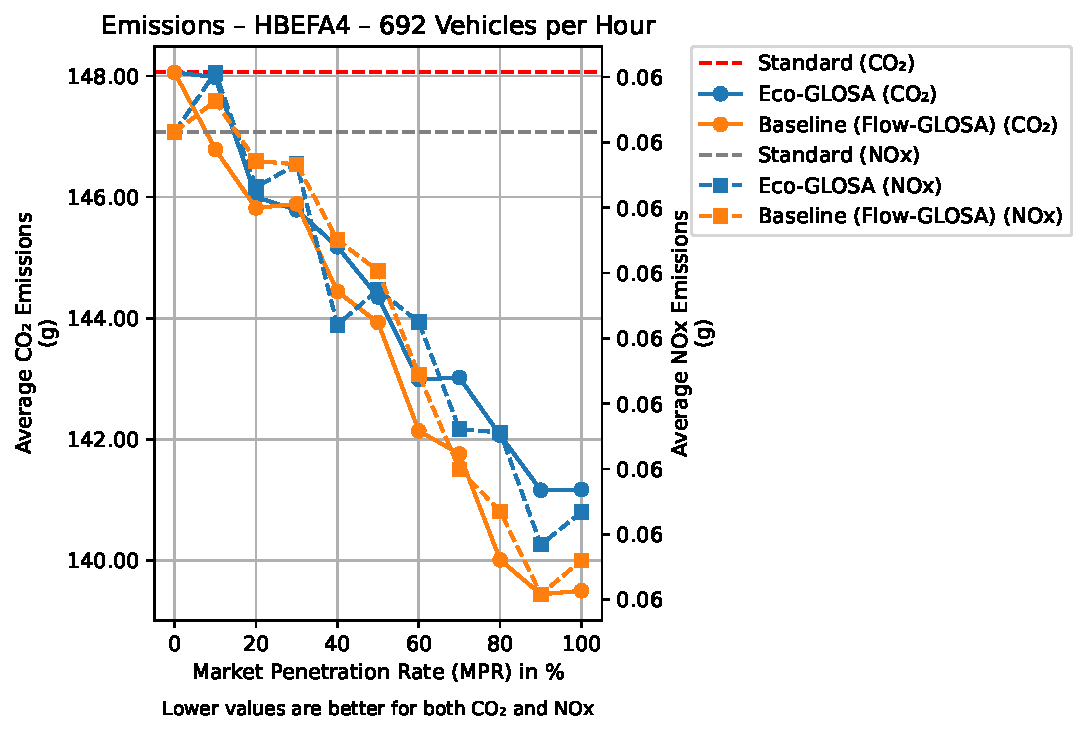
\includegraphics[width=\textwidth]{data/img/Emissions/Emissions_HBEFA4_Cars692.pdf}
    \caption{HBEFA4 at $692\,\mathrm{veh/h}$.}
    \label{fig:Emis_692_HBEFA4}
  \end{subfigure}\hfill
  \begin{subfigure}[b]{0.45\textwidth}
    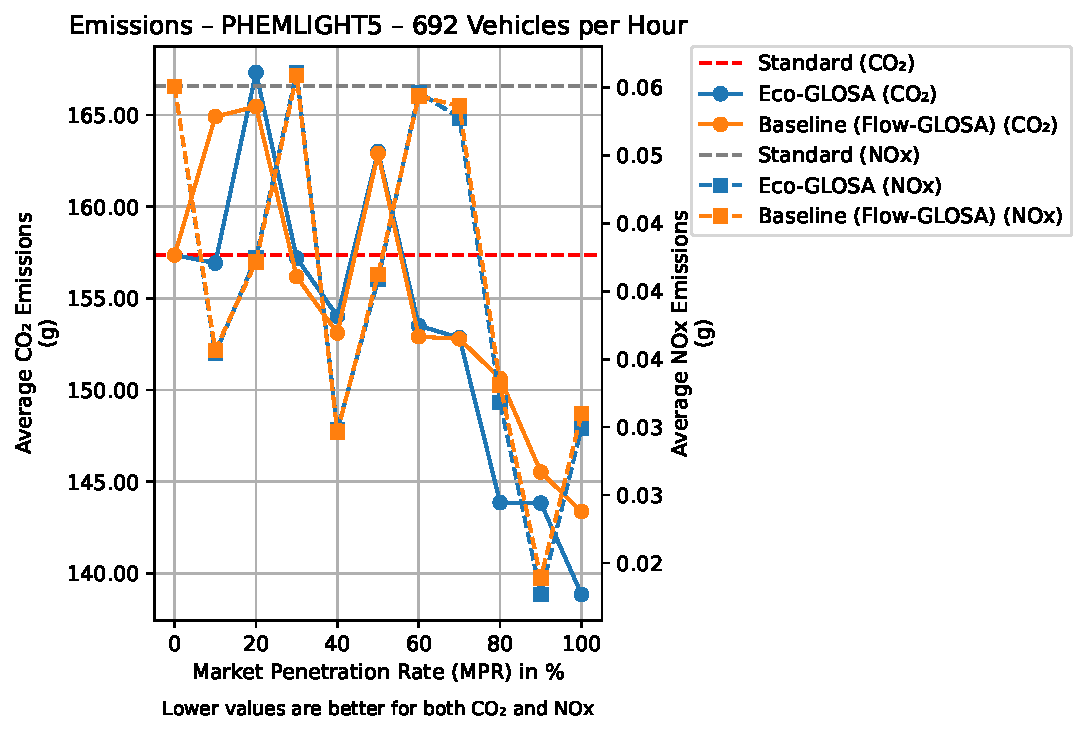
\includegraphics[width=\textwidth]{data/img/Emissions/Emissions_PHEMLIGHT5_Cars692.pdf}
    \caption{PHEMlight5 at $692\,\mathrm{veh/h}$.}
    \label{fig:Emis_692_PHEM}
  \end{subfigure}
  \caption[\ac{co2} and \ac{nox} emissions vs. \ac{mpr} at $692~\unit{\veh\per\hour}$]{\ac{co2} and \ac{nox} emissions versus \ac{mpr} at a low demand of $692~\unit{\veh\per\hour}$.}
\label{fig:Emis_692}
\end{figure}

\paragraph{Emerging Congestion ($1385$--$2077~\unit{\veh\per\hour}$).}
As traffic demand enters the range of emerging congestion, the \ac{eco-glosa} controller begins to realize tangible emission savings, particularly with the HBEFA4 model. At a demand of $1385~\unit{\veh\per\hour}$, the algorithm lowers \ac{co2} emissions from the Standard of $149.86~\unit{\gram\per\kilo\metre}$ to $131.05~\unit{\gram\per\kilo\metre}$ at $80\%$ \ac{mpr}, a reduction of $12.5\%$. This benefit is accompanied by a substantial decrease in \ac{nox} emissions from $0.0584$ to $0.0145~\unit{\gram\per\kilo\metre}$. Comparable gains are observed at $2077~\unit{\veh\per\hour}$, where full penetration of \ac{eco-glosa} reduces \ac{co2} by $12.8\%$ and \ac{nox} by a significant $77.6\%$.
\mynewline
The PHEMlight5 model demonstrates the same qualitative trend, although the magnitude of the savings is attenuated. In the $2077~\unit{\veh\per\hour}$ scenario, \ac{co2} emissions decrease from a baseline of $162.83~\unit{\gram\per\kilo\metre}$ to $154.31~\unit{\gram\per\kilo\metre}$ at $100\%$ \ac{mpr}, a more modest reduction of $5.2\%$. A comparison of the results in Figures~\vref{fig:Emis_2077_HBEFA4} and \vref{fig:Emis_2077_PHEM} corroborates this difference, suggesting the higher transient fidelity of the PHEMlight5 model provides a more conservative estimate of the achievable benefits.

\begin{figure}[htb]
  \centering
  \begin{subfigure}[b]{0.45\textwidth}
    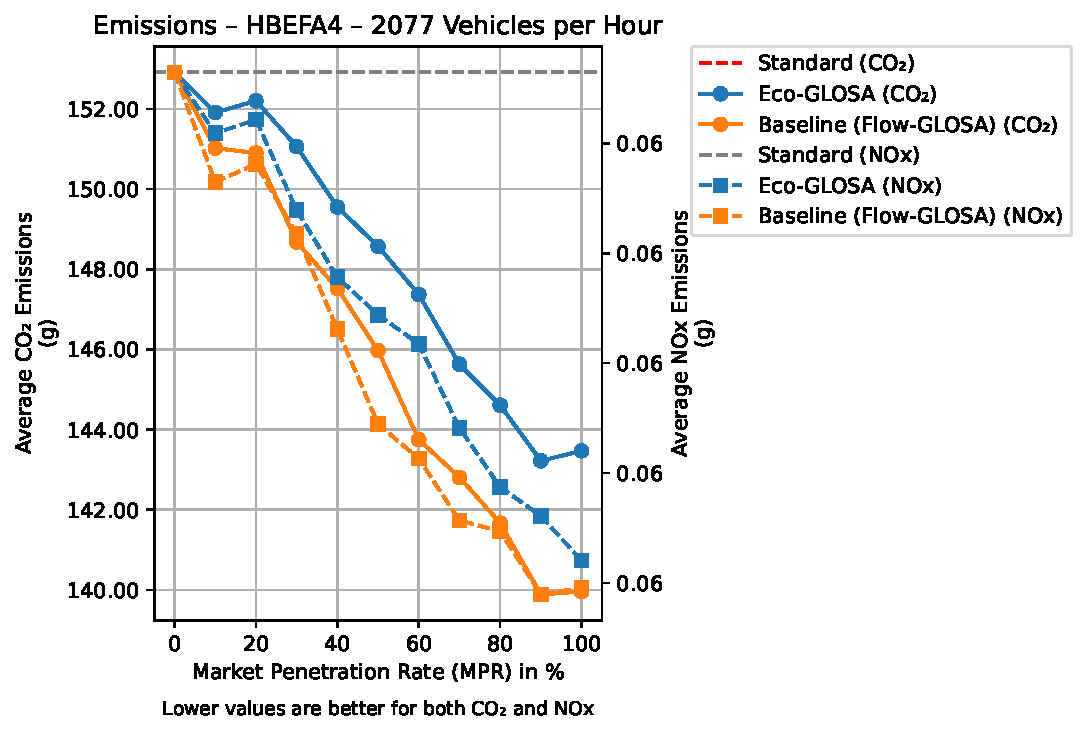
\includegraphics[width=\textwidth]{data/img/Emissions/Emissions_HBEFA4_Cars2077.pdf}
    \caption{HBEFA4 at $2077\,\mathrm{veh/h}$.}
    \label{fig:Emis_2077_HBEFA4}
  \end{subfigure}\hfill
  \begin{subfigure}[b]{0.45\textwidth}
    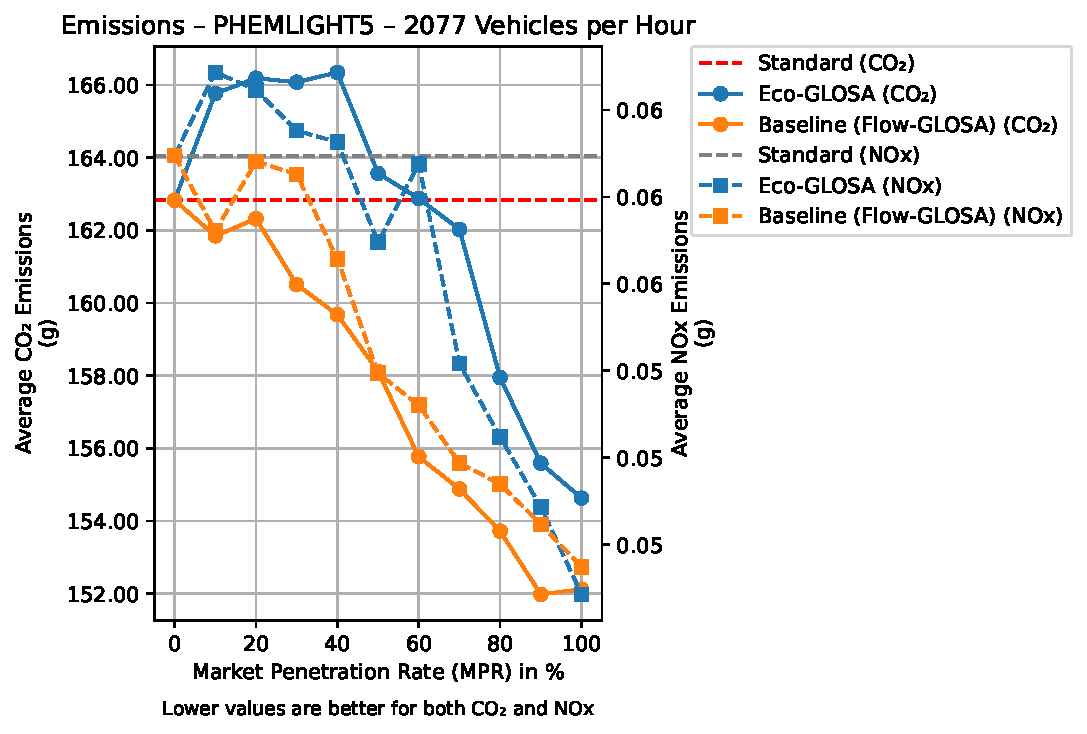
\includegraphics[width=\textwidth]{data/img/Emissions/Emissions_PHEMLIGHT5_Cars2077.pdf}
    \caption{PHEMlight5 at $2077\,\mathrm{veh/h}$.}
    \label{fig:Emis_2077_PHEM}
  \end{subfigure}
  \caption[\ac{co2} and \ac{nox} emissions vs. \ac{mpr} at $2077~\unit{\veh\per\hour}$]{\ac{co2} and \ac{nox} emissions versus \ac{mpr} under emerging congestion at $2077~\unit{\veh\per\hour}$.}
  \label{fig:Emis_2077}
\end{figure}

\paragraph{High Demand ($2769~\unit{\veh\per\hour}$).}
The demand level of $2769~\unit{\veh\per\hour}$ represents a critical turning point for the HBEFA4 model, where the \ac{eco-glosa} controller's performance collapses at moderate penetration rates. Instead of improvements, this leads to enormous emission spikes. The most severe outlier occurs at $60\%$ \ac{mpr}, where \ac{co2} emissions jump to $419.09~\unit{\gram\per\kilo\metre}$ and \ac{nox} emissions to $0.173~\unit{\gram\per\kilo\metre}$, representing increases of $164\%$ and $159\%$ over the Standard, respectively. A secondary peak in \ac{co2} emissions of $270.93~\unit{\gram\per\kilo\metre}$ is already present at $30\%$ \ac{mpr}. As seen in Figure~\vref{fig:Emis_2769_HBEFA4}, these excursions correspond to severe stop-and-go waves. In contrast, the \ac{flow-glosa} controller's emissions remain bounded and consistently below the Standard, showcasing its superior stability.
\mynewline
Under the PHEMlight5 model, the traffic jam is fully established at this demand, leading to poor performance for the \ac{eco-glosa} controller across all penetration rates. Its \ac{co2} emissions rise from the Standard of $168.29~\unit{\gram\per\kilo\metre}$ to a peak of $347.73~\unit{\gram\per\kilo\metre}$ at $70\%$ \ac{mpr}. Unlike the erratic spikes seen in the HBEFA4 model, PHEMlight5 predicts a more uniformly high emission profile for \ac{eco-glosa} in this congested state. This disparity stems from the PHEMlight5 model’s detailed transient engine maps, which impose a steep penalty on the inefficient, low-speed, high-load conditions that characterize a persistent traffic jam. As vehicles repeatedly accelerate from a standstill, their engines are forced into inefficient operating zones, inflating both fuel burn and \ac{nox} formation far beyond the forecasts of the HBEFA4 model.

\begin{figure}[htb]
  \centering
  \begin{subfigure}[b]{0.45\textwidth}
    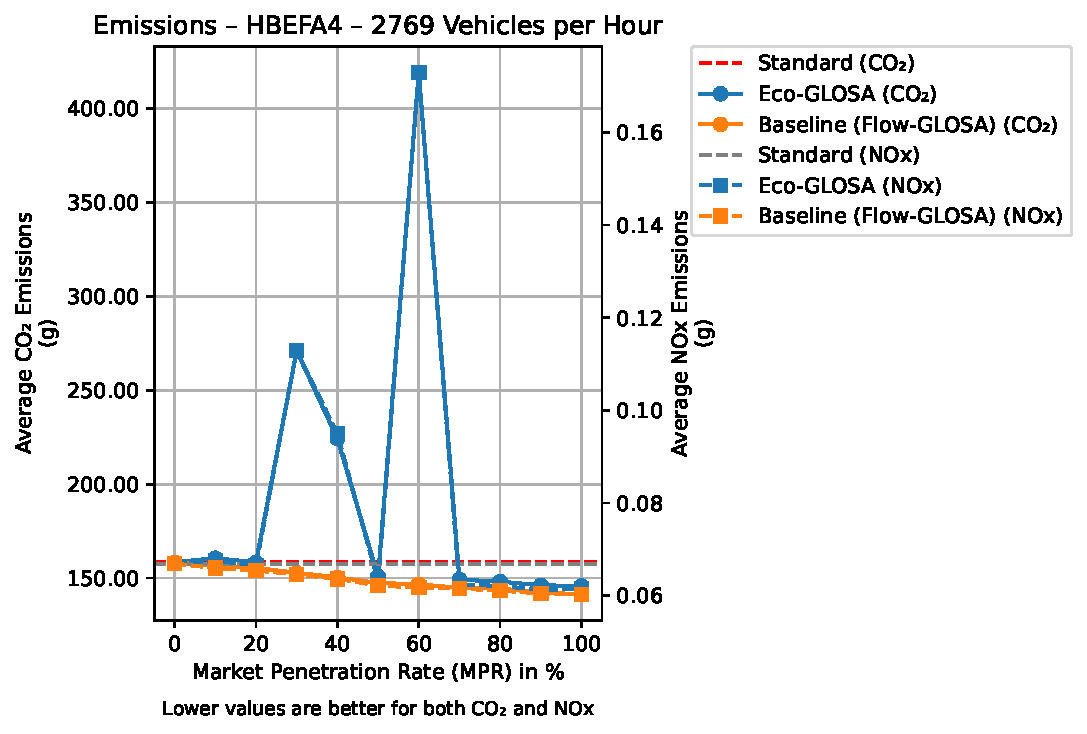
\includegraphics[width=\textwidth]{data/img/Emissions/Emissions_HBEFA4_Cars2769.pdf}
    \caption{HBEFA4 at $2769\,\mathrm{veh/h}$.}
    \label{fig:Emis_2769_HBEFA4}
  \end{subfigure}\hfill
  \begin{subfigure}[b]{0.45\textwidth}
    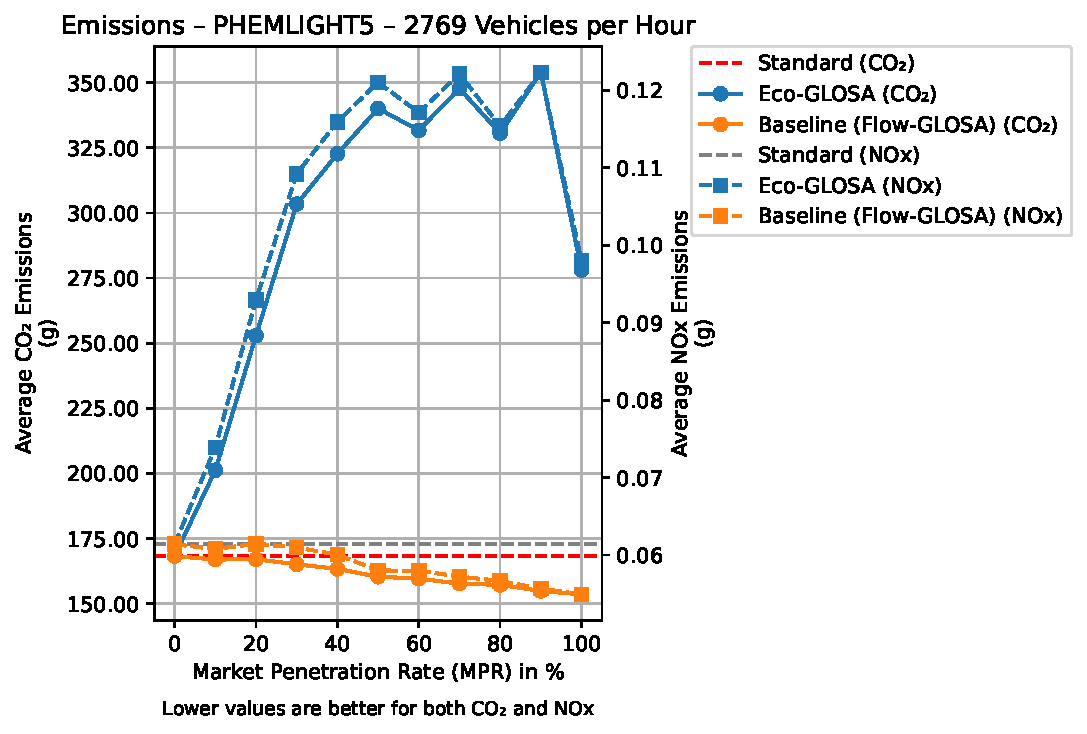
\includegraphics[width=\textwidth]{data/img/Emissions/Emissions_PHEMLIGHT5_Cars2769.pdf}
    \caption{PHEMlight5 at $2769\,\mathrm{veh/h}$.}
    \label{fig:Emis_2769_PHEM}
  \end{subfigure}
  \caption[\ac{co2} and \ac{nox} emissions vs. \ac{mpr} at $2769~\unit{\veh\per\hour}$]{\ac{co2} and \ac{nox} emissions versus \ac{mpr} at a high demand of $2769~\unit{\veh\per\hour}$, showing significant performance degradation for \ac{eco-glosa}.}
  \label{fig:Emis_2769}
\end{figure}

\paragraph{Saturated Regime ($3462~\unit{\veh\per\hour}$).}
The dichotomy between the two control philosophies is most striking in the fully saturated scenario, as shown in Figure~\vref{fig:Emis_3462}. Under the HBEFA4 model, the \ac{eco-glosa} controller consistently degrades performance as penetration increases. Its \ac{co2} emissions soar from the already high Standard of $426.68~\unit{\gram\per\kilo\metre}$ to a peak of $607.47~\unit{\gram\per\kilo\metre}$ at $80\%$ \ac{mpr}. Simultaneously, \ac{nox} emissions escalate dramatically from $0.175$ to $1.325~\unit{\gram\per\kilo\metre}$ at full penetration. This poor performance can be attributed to the controller's logic, which prioritises reaching the intersection for a green light, forcing futile and aggressive accelerations within an existing jam.
\mynewline
Conversely, the \ac{flow-glosa} controller drives the traffic jam to extinction. Under HBEFA4, its application causes \ac{co2} emissions to plummet from $426.68~\unit{\gram\per\kilo\metre}$ to just $151.33~\unit{\gram\per\kilo\metre}$ at $100\%$ \ac{mpr}. Once the queue clears, emissions settle on a plateau as vehicles traverse the corridor at a stable free-flow speed. This advantage is even more pronounced with the PHEMlight5 model. At full penetration, \ac{eco-glosa} still produces $367.78~\unit{\gram\per\kilo\metre}$ of \ac{co2}, whereas \ac{flow-glosa} emits only $152.59~\unit{\gram\per\kilo\metre}$. The absolute difference of $215.19~\unit{\gram\per\kilo\metre}$ represents a performance factor of $2.4$ in favour of the \ac{flow-glosa} strategy. A similar ratio is observed for \ac{nox} emissions ($0.829$ versus $0.341~\unit{\gram\per\kilo\metre}$). These findings reveal that a control law aimed at maximising throughput can dramatically outperform an ostensibly eco-oriented variant in heavily congested traffic.

\begin{figure}[htb]
  \centering
  \begin{subfigure}[b]{0.45\textwidth}
    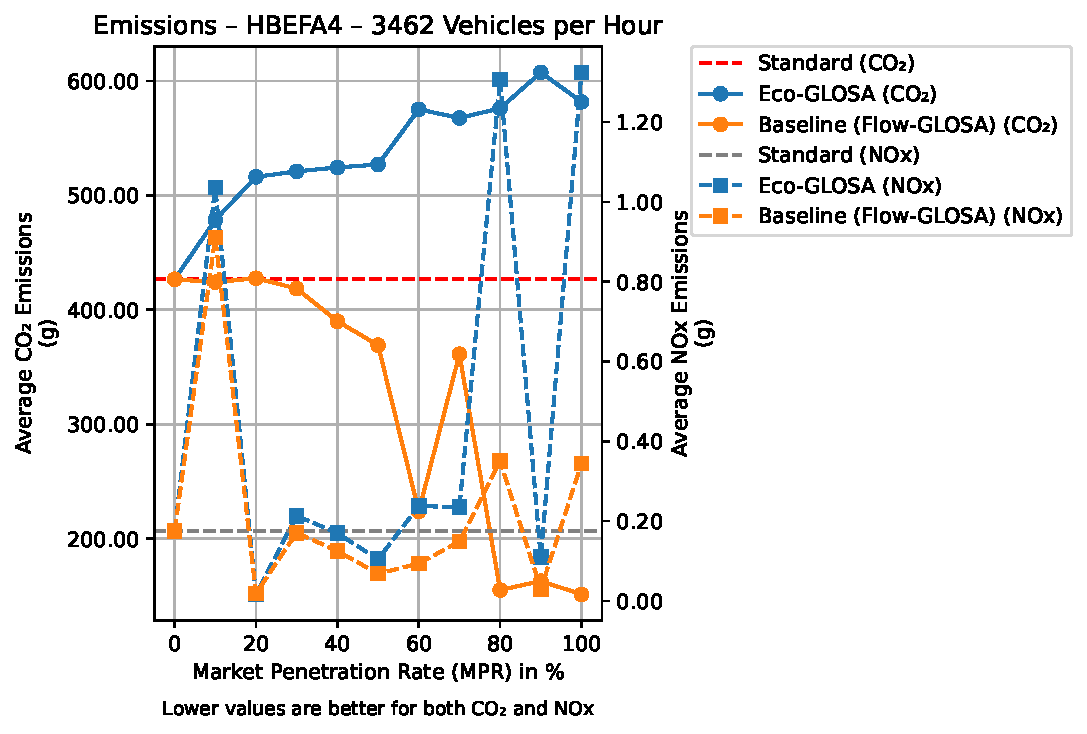
\includegraphics[width=\textwidth]{data/img/Emissions/Emissions_HBEFA4_Cars3462.pdf}
    \caption{HBEFA4 at $3462\,\mathrm{veh/h}$.}
    \label{fig:Emis_3462_HBEFA4}
  \end{subfigure}\hfill
  \begin{subfigure}[b]{0.45\textwidth}
    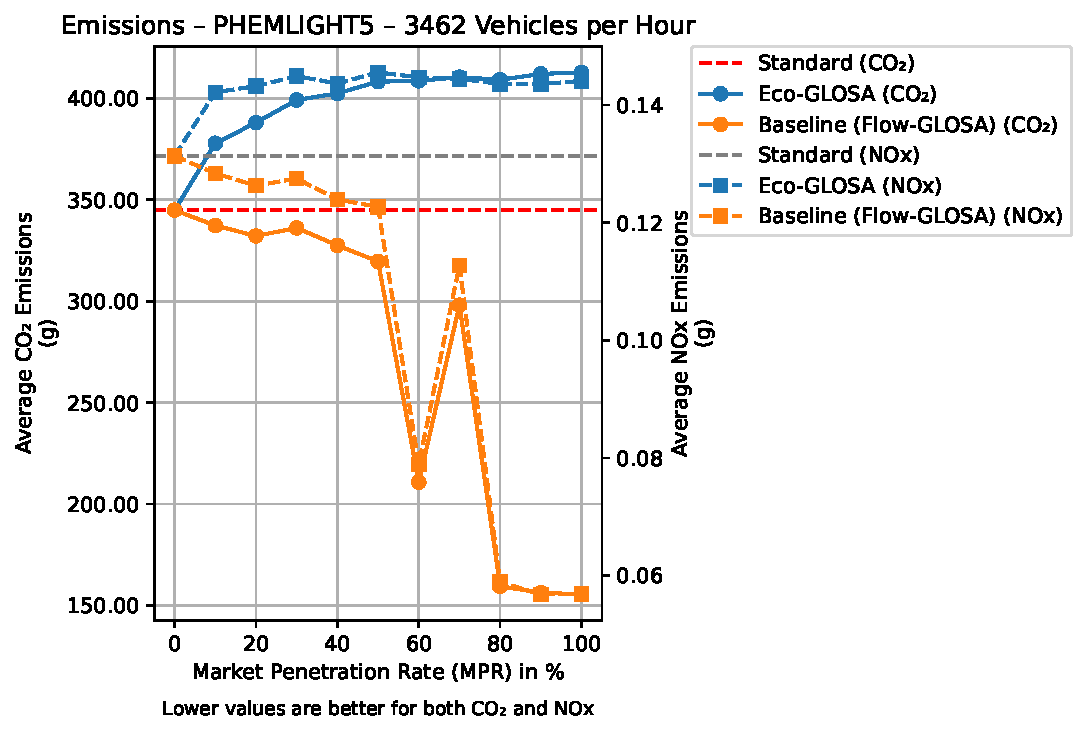
\includegraphics[width=\textwidth]{data/img/Emissions/Emissions_PHEMLIGHT5_Cars3462.pdf}
    \caption{PHEMlight5 at $3462\,\mathrm{veh/h}$.}
    \label{fig:Emis_3462_PHEM}
  \end{subfigure}
  \caption[\ac{co2} and \ac{nox} emissions vs. \ac{mpr} at $3462~\unit{\veh\per\hour}$]{\ac{co2} and \ac{nox} emissions versus \ac{mpr} in the fully saturated regime ($3462~\unit{\veh\per\hour}$), highlighting the superior performance of \ac{flow-glosa}.}
  \label{fig:Emis_3462}
\end{figure}

\paragraph{Inter-Model Comparison.}
Juxtaposing the HBEFA4 and PHEMlight5 models reveals two key differences in their predictions. First, they provide different estimates of the absolute benefits of \ac{flow-glosa} in saturation. For the $3462~\unit{\veh\per\hour}$ scenario, HBEFA4 predicts a \ac{co2} reduction of approximately $64\%$, while PHEMlight5 estimates a more conservative, though still substantial, $56\%$ reduction. This discrepancy arises because the Standard (baseline) emission value for HBEFA4 is inflated by more than $80~\unit{\gram\per\kilo\metre}$ compared to PHEMlight5, suggesting its static drive-cycle factors may inadequately capture engine behaviour during prolonged idling.
\mynewline
Second, the models diverge in their sensitivity to the performance degradation of \ac{eco-glosa} in congested traffic. At $2769~\unit{\veh\per\hour}$, the PHEMlight5 model shows that \ac{eco-glosa} becomes detrimental almost immediately, yielding higher emissions than \ac{flow-glosa} from just $10\%$ \ac{mpr} onwards. The HBEFA4 results are more volatile, showing severe emission spikes at certain penetration rates rather than a consistent trend. The earlier and more consistent penalty from PHEMlight5 is likely explained by its more granular power-band binning, which better captures the inefficiency of the aggressive, transient manoeuvres induced by \ac{eco-glosa} in dense traffic.

\paragraph{Key Conclusions on Emissions.}
The emission analysis reveals that a single \ac{glosa} strategy is not universally optimal; performance is highly dependent on traffic density. In under-saturated traffic, the emission impact is often dominated by stochastic effects, with neither controller showing a consistent advantage. As congestion becomes moderate, both algorithms can reduce \ac{co2} and \ac{nox} emissions, with \ac{eco-glosa} offering the greatest potential improvements provided that traffic oscillations remain mild.
\mynewline
Beyond a critical volume threshold, however, the myopic nature of the \ac{eco-glosa} controller becomes a significant liability. Its focus on individual vehicle efficiency amplifies stop-and-go waves, in some cases more than doubling emissions. This effect is so pronounced that, particularly when evaluated with the sensitive PHEMlight5 model, the introduction of \ac{eco-glosa} can \textit{induce a severe traffic jam} in conditions that would otherwise remain free-flowing. In these high-density scenarios, a throughput-centered strategy like \ac{flow-glosa} proves superior. By resolving the jam entirely at an \ac{mpr} of $80\%$ or higher, it can cut emissions by over $60\%$ compared to the Standard case. Ultimately, the choice of emission model is critical, as the higher fidelity of PHEMlight5 predicts these performance shifts more accurately than the HBEFA4 model.
\mynewline
This underscores a key methodological paradox concerning the choice of emission model. The high physical fidelity of PHEMlight5 accurately penalises the severe energy cost of transient, stop-and-go manoeuvres. In response, the \ac{eco-glosa} controller, in its strict pursuit of minimising fuel use, advises overly conservative speed profiles to avoid these high-cost states. Paradoxically, this locally optimal strategy is what induces severe network-level congestion, creating traffic jams where none existed and ultimately leading to far higher system-wide emissions. In contrast, the HBEFA4 model's relative insensitivity to these transient states leads to speed advisories that, while less \enquote{eco-optimal} in a narrow sense, are more compatible with maintaining traffic flow. The result is that the less accurate model, when paired with the \ac{eco-glosa} controller, leads to a better overall environmental outcome precisely because it prevents the controller from making decisions that are disastrous for network stability. This finding suggests that a successful eco-driving controller must balance high-fidelity physical models with robust, network-level traffic flow objectives to prevent locally optimal choices from causing globally detrimental effects.

\begin{table}[htb]
  \centering
  \caption[Average \ac{co2} and \ac{nox} emissions for all traffic volumes and \acp{mpr}]{Vehicle emissions in terms of average \ac{co2} ($\unit{\gram\per\kilo\metre}$) and \ac{nox} ($\unit{\gram\per\kilo\metre}$) for all traffic volumes and \acp{mpr}. The data compares the Standard, \ac{flow-glosa}, and \ac{eco-glosa} configurations.}
  \label{tab:Emissions}
  \resizebox{\textwidth}{!}{%
    \begin{tabular}{l l l *{11}{c}}
      \toprule
      Vehicles & Algorithm                & Fuel         & \textbf{0 \% (Standard)} & 10 \%     & 20 \%     & 30 \%       & 40 \%       & 50 \%       & 60 \%       & 70 \%       & 80 \%       & 90 \%       & 100 \%      \\
      \midrule
      69.0 & Eco-GLOSA                 & HBEFA4       & \textbf{149.99,0.0606}   & 164.05,0.03 & 169.37,0.0345 & 144.59,0.0582 & \textbf{127.88,0.0167} & 165.55,0.0342 & 143.45,0.0549 & 141.49,0.0555 & 154.28,0.0286 & 147.82,0.355  & 153.20,0.3521 \\
      69.0 & Baseline (Flow-GLOSA)     & HBEFA4       & \textbf{149.99,0.0606}   & 164.58,0.0302 & 171.67,0.0349 & 145.27,0.0588 & 128.53,0.0171 & 162.00,0.0332 & 145.08,0.0563 & 140.88,0.0548 & 153.86,0.0287 & 145.60,0.3528 & 149.80,0.3543 \\
      69.0 & Eco-GLOSA                 & PHEMlight5   & \textbf{155.51,0.0586}   & 156.20,0.0331 & \textbf{148.83,0.0358} & 148.37,0.0515 & 142.98,0.0199 & \textbf{131.45,0.0312} & 149.17,0.0552 & 144.54,0.0493 & 138.25,0.0296 & 136.50,0.3026 & 137.57,0.3034 \\
      69.0 & Baseline (Flow-GLOSA)     & PHEMlight5   & \textbf{155.51,0.0586}   & 150.06,0.0328 & 148.80,0.0367 & 150.51,0.0534 & 145.63,0.0215 & 138.77,0.0330 & 150.43,0.0531 & 147.89,0.0504 & 139.57,0.0291 & 141.36,0.3147 & 154.08,0.3891 \\
      \midrule
      138.0 & Eco-GLOSA                & HBEFA4       & \textbf{148.70,0.0653}   & 158.42,0.3739 & 142.81,0.0521 & 144.14,0.0660 & 142.15,0.0172 & 131.18,0.0215 & 141.96,0.0650 & 140.59,0.0634 & 161.97,0.3757 & 163.17,0.0337 & 146.68,0.3450 \\
      138.0 & Baseline (Flow-GLOSA)    & HBEFA4       & \textbf{148.70,0.0653}   & 151.97,0.3579 & 143.07,0.0522 & 145.54,0.0669 & 137.95,0.0169 & 133.02,0.0216 & 141.83,0.0661 & 139.88,0.0638 & 157.35,0.3669 & 168.69,0.0342 & 147.16,0.3522 \\
      138.0 & Eco-GLOSA                & PHEMlight5   & \textbf{155.28,0.0603}   & 155.68,0.3546 & 162.40,0.0403 & 149.91,0.0623 & 151.66,0.0208 & 144.26,0.0185 & 148.81,0.0583 & 147.75,0.0577 & 150.13,0.3467 & 136.40,0.0323 & 142.41,0.3166 \\
      138.0 & Baseline (Flow-GLOSA)    & PHEMlight5   & \textbf{155.28,0.0603}   & 150.74,0.3583 & 160.31,0.0409 & 153.54,0.0635 & 153.58,0.0224 & 148.65,0.0185 & 150.68,0.0638 & 148.26,0.0610 & 156.77,0.3734 & 144.61,0.0352 & 145.27,0.3295 \\
      \midrule
      346.0 & Eco-GLOSA                & HBEFA4       & \textbf{147.86,0.0613}   & 166.00,0.0303 & 135.38,0.0165 & 147.48,0.0607 & 153.16,0.3518 & 131.61,0.0150 & 142.92,0.0591 & 144.14,0.0596 & 159.45,0.0293 & 168.06,0.0348 & 162.48,0.0337 \\
      346.0 & Baseline (Flow-GLOSA)    & HBEFA4       & \textbf{147.86,0.0613}   & 164.34,0.0301 & 137.57,0.0163 & 146.00,0.0605 & 151.92,0.3526 & 132.37,0.0158 & 142.70,0.0592 & 142.98,0.0597 & 156.50,0.0288 & 166.58,0.0348 & 162.83,0.0342 \\
      346.0 & Eco-GLOSA                & PHEMlight5   & \textbf{156.60,0.0565}   & 143.04,0.0307 & 147.53,0.0193 & 155.81,0.0555 & 153.46,0.3496 & 147.79,0.0177 & 151.95,0.0540 & 151.23,0.0533 & 143.46,0.0302 & 141.59,0.0341 & 143.35,0.0348 \\
      346.0 & Baseline (Flow-GLOSA)    & PHEMlight5   & \textbf{156.60,0.0565}   & 151.50,0.0326 & 152.03,0.0201 & 155.66,0.0570 & 150.87,0.3398 & 147.92,0.0181 & 152.34,0.0549 & 152.69,0.0553 & 145.78,0.0311 & 147.78,0.0358 & 145.27,0.0356 \\
      \midrule
      692.0 & Eco-GLOSA                & HBEFA4       & \textbf{148.06,0.0611}   & 168.31,0.0314 & 146.24,0.0533 & 145.79,0.0608 & 139.15,0.0397 & 143.76,0.0524 & 142.99,0.0596 & 143.02,0.0588 & 166.96,0.0306 & 144.01,0.0141 & 161.09,0.0298 \\
      692.0 & Baseline (Flow-GLOSA)    & HBEFA4       & \textbf{148.06,0.0611}   & 179.99,0.0336 & 147.31,0.0537 & 145.89,0.0608 & 138.17,0.0393 & 144.78,0.0529 & 142.14,0.0592 & 141.76,0.0585 & 161.27,0.0299 & 141.95,0.0146 & 155.71,0.0287 \\
      692.0 & Eco-GLOSA                & PHEMlight5   & \textbf{157.36,0.0551}   & 156.92,0.0354 & 167.32,0.0424 & 157.20,0.0561 & 154.02,0.0298 & 163.01,0.0409 & 153.51,0.0546 & 152.85,0.0528 & 143.86,0.0318 & 143.84,0.0177 & 138.86,0.0299 \\
      692.0 & Baseline (Flow-GLOSA)    & PHEMlight5   & \textbf{157.36,0.0551}   & 164.91,0.0357 & 165.46,0.0422 & 156.18,0.0559 & 153.11,0.0297 & 162.90,0.0412 & 152.91,0.0544 & 152.79,0.0536 & 150.63,0.0331 & 145.53,0.0189 & 143.37,0.0310 \\
      \midrule
      1385.0 & Eco-GLOSA               & HBEFA4       & \textbf{149.86,0.0584}   & 137.88,0.0167 & 141.17,0.0403 & 147.99,0.0573 & 150.72,0.0157 & 153.69,0.3545 & 145.46,0.0562 & 144.34,0.0558 & 131.05,0.0145 & 167.72,0.0344 & \textbf{130.39,0.0141} \\
      1385.0 & Baseline (Flow-GLOSA)   & HBEFA4       & \textbf{149.86,0.0584}   & 138.62,0.0165 & 140.78,0.0402 & 147.28,0.0575 & 148.88,0.0156 & 153.32,0.3530 & 143.28,0.0561 & 142.33,0.0555 & 130.39,0.0155 & 168.69,0.0349 & 128.27,0.0154 \\
      1385.0 & Eco-GLOSA               & PHEMlight5   & \textbf{159.38,0.0528}   & 156.69,0.0206 & 158.86,0.0307 & 162.99,0.0548 & 156.69,0.0217 & 158.01,0.3604 & 160.70,0.0533 & 157.58,0.0508 & 154.07,0.0182 & 150.49,0.0365 & \textbf{148.21,0.0164} \\
      1385.0 & Baseline (Flow-GLOSA)   & PHEMlight5   & \textbf{159.38,0.0528}   & 155.23,0.0210 & 155.04,0.0300 & 158.16,0.0532 & 151.80,0.0209 & 153.21,0.3538 & 154.51,0.0519 & 153.93,0.0509 & 148.74,0.0187 & 149.63,0.0360 & 146.85,0.0180 \\
      \midrule
      2077.0 & Eco-GLOSA               & HBEFA4       & \textbf{152.91,0.0616}   & 141.32,0.0163 & 171.95,0.0317 & 151.06,0.0604 & 158.07,0.3611 & 157.57,0.3599 & 147.37,0.0592 & 145.63,0.0584 & 132.87,0.0138 & 145.67,0.0138 & \textbf{133.30,0.0138} \\
      2077.0 & Baseline (Flow-GLOSA)   & HBEFA4       & \textbf{152.91,0.0616}   & 141.43,0.0161 & 168.98,0.0314 & 148.68,0.0602 & 157.28,0.3600 & 153.32,0.3523 & 143.75,0.0581 & 142.81,0.0576 & 131.22,0.0153 & 143.94,0.0145 & 129.17,0.0152 \\
      2077.0 & Eco-GLOSA               & PHEMlight5   & \textbf{162.83,0.0565}   & 162.24,0.0215 & 165.20,0.0369 & 166.08,0.0568 & 161.99,0.3670 & 159.59,0.3623 & 162.88,0.0564 & 162.03,0.0541 & 157.46,0.0180 & 152.18,0.0185 & \textbf{154.31,0.0163} \\
      2077.0 & Baseline (Flow-GLOSA)   & PHEMlight5   & \textbf{162.83,0.0565}   & 158.18,0.0207 & 157.42,0.0348 & 160.51,0.0563 & 158.86,0.3637 & 154.02,0.3506 & 155.77,0.0536 & 154.88,0.0529 & 150.66,0.0189 & 148.04,0.0195 & 148.71,0.0182 \\
      \midrule
      2769.0 & Eco-GLOSA               & HBEFA4       & \textbf{158.44,0.0669}   & 149.68,0.0165 & 150.27,0.0438 & \textbf{270.93,0.1129} & 223.93,0.0152 & 144.07,0.0419 & \textbf{419.09,0.1730} & 149.20,0.0624 & 136.94,0.0136 & 137.47,0.0233 & \textbf{134.94,0.0131} \\
      2769.0 & Baseline (Flow-GLOSA)   & HBEFA4       & \textbf{158.44,0.0669}   & 144.45,0.0163 & 148.28,0.0431 & 152.84,0.0646 & 155.17,0.0153 & 140.40,0.0405 & 146.67,0.0617 & 144.90,0.0615 & 133.43,0.0148 & 134.78,0.0224 & 131.03,0.0145 \\
      2769.0 & Eco-GLOSA               & PHEMlight5   & \textbf{168.29,0.0614}   & 191.39,0.0278 & 232.01,0.0462 & 303.40,0.1092 & 284.24,0.0441 & 306.10,0.0621 & 331.67,0.1171 & \textbf{347.73,0.1221} & 295.95,0.0404 & 321.37,0.0433 & \textbf{255.90,0.0318} \\
      2769.0 & Baseline (Flow-GLOSA)   & PHEMlight5   & \textbf{168.29,0.0614}   & 161.20,0.0215 & 162.91,0.0316 & 165.15,0.0610 & 158.91,0.0223 & 157.16,0.0305 & 159.67,0.0580 & 157.75,0.0572 & 153.28,0.0188 & 153.69,0.0194 & 150.97,0.0179 \\
      \midrule
      3462.0 & Eco-GLOSA               & HBEFA4       & \textbf{426.68,0.1747}   & 478.55,1.0357 & 516.15,0.0163 & 520.98,0.2133 & 524.40,0.1698 & 526.96,0.1042 & 575.15,0.2378 & 567.63,0.2347 & \textbf{607.47,0.1096} & 581.74,0.1096 & \textbf{581.74,1.3247} \\
      3462.0 & Baseline (Flow-GLOSA)   & HBEFA4       & \textbf{426.68,0.1747}   & 424.17,0.9106 & 427.59,0.0187 & 418.54,0.1707 & 389.99,0.1248 & 369.14,0.0681 & \textbf{223.84,0.0933} & 361.16,0.1486 & \textbf{155.09,0.3505} & \textbf{162.90,0.0296} & \textbf{151.33,0.3443} \\
      3462.0 & Eco-GLOSA               & PHEMlight5   & \textbf{344.88,0.1313}   & 361.38,0.8343 & 343.20,0.0563 & 399.19,0.1449 & 357.12,0.0729 & 369.50,0.0461 & 408.63,0.1447 & 410.45,0.1445 & \textbf{364.90,0.8214} & 359.41,0.0796 & \textbf{367.78,0.8285} \\
      3462.0 & Baseline (Flow-GLOSA)   & PHEMlight5   & \textbf{344.88,0.1313}   & 329.05,0.7561 & 299.05,0.0511 & 336.12,0.1275 & 297.39,0.0604 & 297.18,0.0321 & 210.82,0.0789 & 298.02,0.1127 & \textbf{156.83,0.3529} & \textbf{151.75,0.0330} & \textbf{152.59,0.3409} \\
      \bottomrule
    \end{tabular}%
  }
\end{table}


\subsection{Break‐Even Penetration Analysis}
\label{sec:Results_BreakEven}

The break-even study identifies the combinations of traffic volume and \ac{mpr} for which \ac{eco-glosa} yields lower mean \ac{co2} emissions than (i) the \ac{flow-glosa} baseline and (ii) the uncontrolled Standard. The numerical results are listed in Tables~\ref{tab:BreakEven_EcoVsFlow} and \ref{tab:BreakEven_EcoVsStd}, while the decision maps are grouped in Figs.~\ref{fig:BE_EcoFlow} and \ref{fig:BE_EcoStd}.

\paragraph{\ac{eco-glosa} versus \ac{flow-glosa}.}
Under HBEFA4, the advantage of \ac{eco-glosa} shrinks as either \ac{mpr} or volume increases. For example, Table~\ref{tab:BreakEven_EcoVsFlow} shows a peak benefit of $+2.30\,\mathrm{g\,km^{-1}}$ at $69\,\mathrm{veh/h}$ and $20\%$ \ac{mpr}; thereafter values oscillate and turn negative beyond $50\%$ penetration. The transition is visible in Fig.~\subref{fig:BE_EcoFlow_HBEFA4}: the green region disappears above the dashed line, indicating that \ac{flow-glosa} becomes preferable once either traffic exceeds $500\,\mathrm{veh/h}$ or penetration surpasses $60\%$. 
\mynewline
PHEMlight5 produces a cleaner separation (Fig.~\subref{fig:BE_EcoFlow_PHEM}): \ac{eco-glosa} dominates below the grey envelope and cedes the advantage above it. Positive margins reach $+8.46$ at $346\,\mathrm{veh/h}$ and $10\%$ penetration, but fall to $-44.15\,\mathrm{g\,km^{-1}}$ at $3462\,\mathrm{veh/h}$ and $20\%$. The steeper penalty for high-demand stems from PHEMlight5’s transient engine map, which amplifies the fuel cost of the sharp accelerations induced by \ac{eco-glosa} when queues build up. A secondary insight is that the break-even curve is almost vertical between $30$ and $60\%$, implying that once penetration exceeds approximately $35\%$ the volume threshold shifts abruptly from $1000$ to $1500\,\mathrm{veh/h}$ with little sensitivity to further penetration increases.

\paragraph{\ac{eco-glosa} versus Standard.}
Figures~\ref{fig:BE_EcoStd} reveal that \ac{eco-glosa} can still outperform the uncontrolled scenario even when it loses to the baseline. For HBEFA4 (Fig.~\subref{fig:BE_EcoStd_HBEFA4}) low and medium volumes show sizeable gains, peaking at $+22.11\,\mathrm{g\,km^{-1}}$ for $69\,\mathrm{veh/h}$ and $40\%$ \ac{mpr}. The green zone narrows with demand and vanishes entirely once a stable jam exists above $2300\,\mathrm{veh/h}$. Under PHEMlight5 (Fig.~\subref{fig:BE_EcoStd_PHEM}) the usable region widens: positive differences appear for almost every \ac{mpr} above $30\%$ up to $1385\,\mathrm{veh/h}$, reaching $+24.06\,\mathrm{g\,km^{-1}}$ at $69\,\mathrm{veh/h}$ and $50\%$ \ac{mpr}. Only the two highest volumes show across-the-board detriment, with a worst case of $-163.38\,\mathrm{g\,km^{-1}}$ at $2769\,\mathrm{veh/h}$ and $60\%$ penetration.

\paragraph{Supplementary Findings.}
\begin{enumerate}
  \item \textit{Optimal penetration depends on demand.}  When traffic is light (below $500\,\mathrm{veh/h}$), each additional \ac{eco-glosa} vehicle delivers its greatest marginal emission reduction in the $10$–$30\%$ penetration range, because the algorithm can smooth vehicle arrivals without creating new stop-go waves. However, once volumes exceed $1000\,\mathrm{veh/h}$, meaningful gains only appear after $50\%$–$80\%$ of vehicles are equipped, since low to moderate penetration fails to overcome the inherent congestion dynamics. In practice, this means that planners deploying \ac{eco-glosa} should prioritise corridors with light to medium load for early rollout, while high-volume arterials require near-universal adoption before benefits materialize.
  \item \textit{Demand amplifies penalties more than partial coverage.}  Negative outcomes (where \ac{eco-glosa} increases emissions) escalate much more rapidly with rising traffic than with penetration rate. For example, at fixed $30\%$ penetration the worst-case CO$_2$ penalty under HBEFA4 grows from about $-19\,\mathrm{g/km}$ at $69\,\mathrm{veh/h}$ to over $-351\,\mathrm{g/km}$ at $3462\,\mathrm{veh/h}$, a nearly $19\times$ increase. By contrast, doubling penetration from $30\%$ to $60\%$ at moderate demand only doubles the penalty magnitude. Thus, network demand is the dominant factor in whether \ac{eco-glosa} will underperform, and flow-based control (\ac{flow-glosa}) is preferable whenever traffic approaches saturation.
\end{enumerate}

\paragraph{Implications for deployment.}
\begin{itemize}
  \item For urban volumes below $700\,\mathrm{veh/h}$, \ac{eco-glosa} becomes beneficial once penetration exceeds roughly $30\%$ (HBEFA4) or $20\%$ (PHEMlight5), offering up to $22\,\mathrm{g\,km^{-1}}$ reduction over the Standard.
  \item In the transition range ($700$–$2000\,\mathrm{veh/h}$) the algorithm should only be chosen at high penetration ($\geq80\%$); otherwise \ac{flow-glosa} is preferable, saving up to $44\,\mathrm{g\,km^{-1}}$ relative to \ac{eco-glosa}.
  \item In saturated corridors ($>2300\,\mathrm{veh/h}$) \ac{flow-glosa} is consistently superior, as its throughput maximisation suppresses stop–go oscillations that dominate fuel use.
\end{itemize}

These thresholds outline the general envelope of traffic volumes and equipment rates within which \ac{eco-glosa} can deliver emission savings, and indicate that beyond this region the throughput‐focused \ac{flow-glosa} is the more reliable choice.  

\begin{figure}[htb]
  \centering
  \begin{subfigure}[b]{0.45\textwidth}
    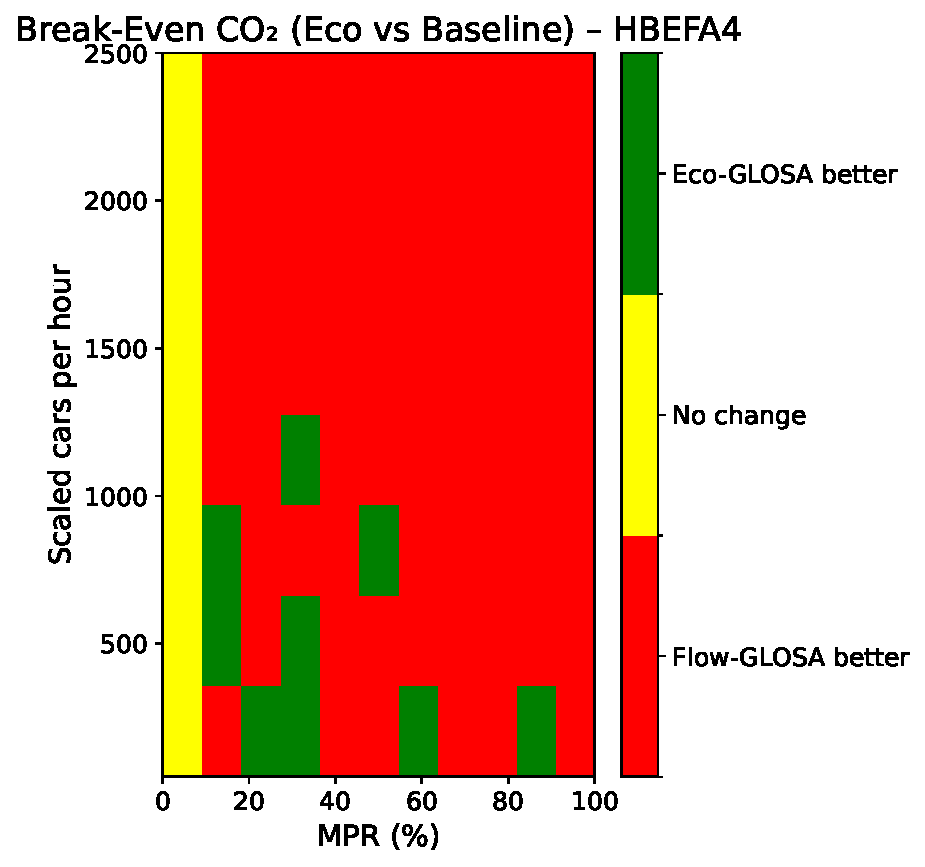
\includegraphics[width=\textwidth]{data/img/BreakEven/BreakEven_CO2_HBEFA4.pdf}
    \caption{HBEFA4 model.}
    \label{fig:BE_EcoFlow_HBEFA4}
  \end{subfigure}\hfill
  \begin{subfigure}[b]{0.45\textwidth}
    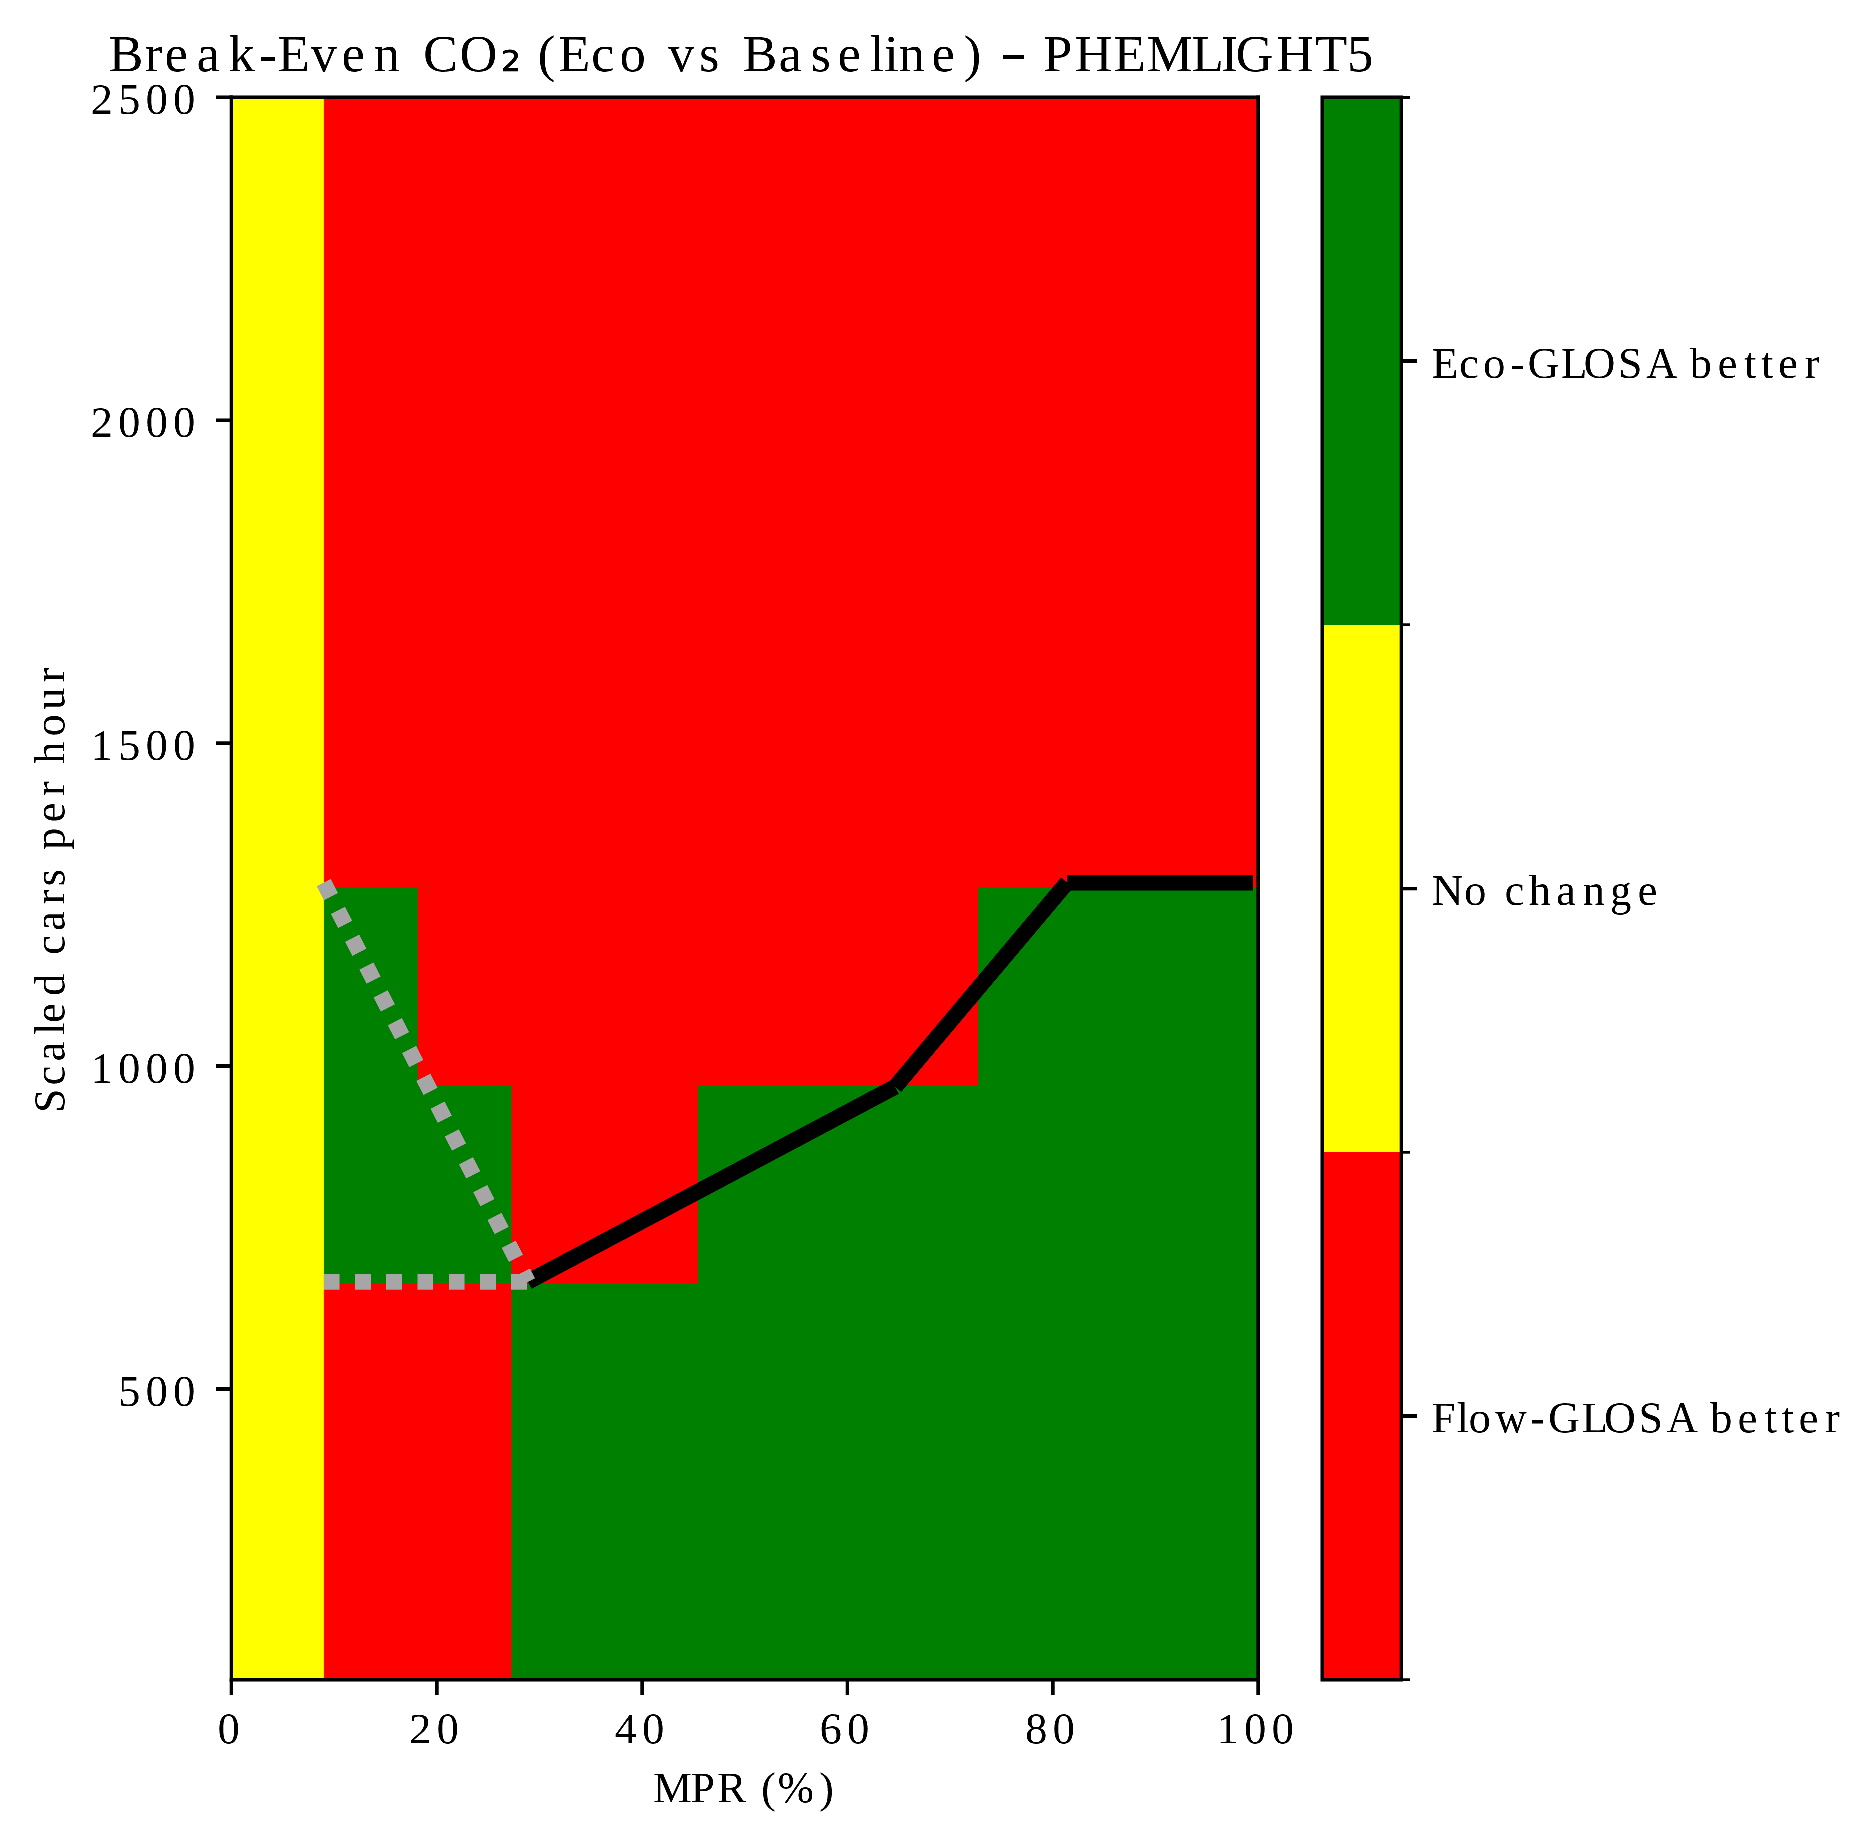
\includegraphics[width=\textwidth]{data/img/BreakEven/BreakEven_CO2_PHEMLIGHT5.pdf}
    \caption{PHEMlight5 model.}
    \label{fig:BE_EcoFlow_PHEM}
  \end{subfigure}
  \caption{Break-even CO$_2$ emission map showing the difference between \ac{eco-glosa} and \ac{flow-glosa}. Green regions indicate parameter combinations where \ac{eco-glosa} yields lower CO$_2$ emissions than \ac{flow-glosa}, while red regions denote scenarios where the baseline is more effective. Grey dashed lines represent the empirical boundary between advantageous regimes, and the solid black curve connects the points of maximum CO$_2$ benefit.}
  \label{fig:BE_EcoFlow}
\end{figure}

\begin{figure}[htb]
  \centering
  \begin{subfigure}[b]{0.45\textwidth}
    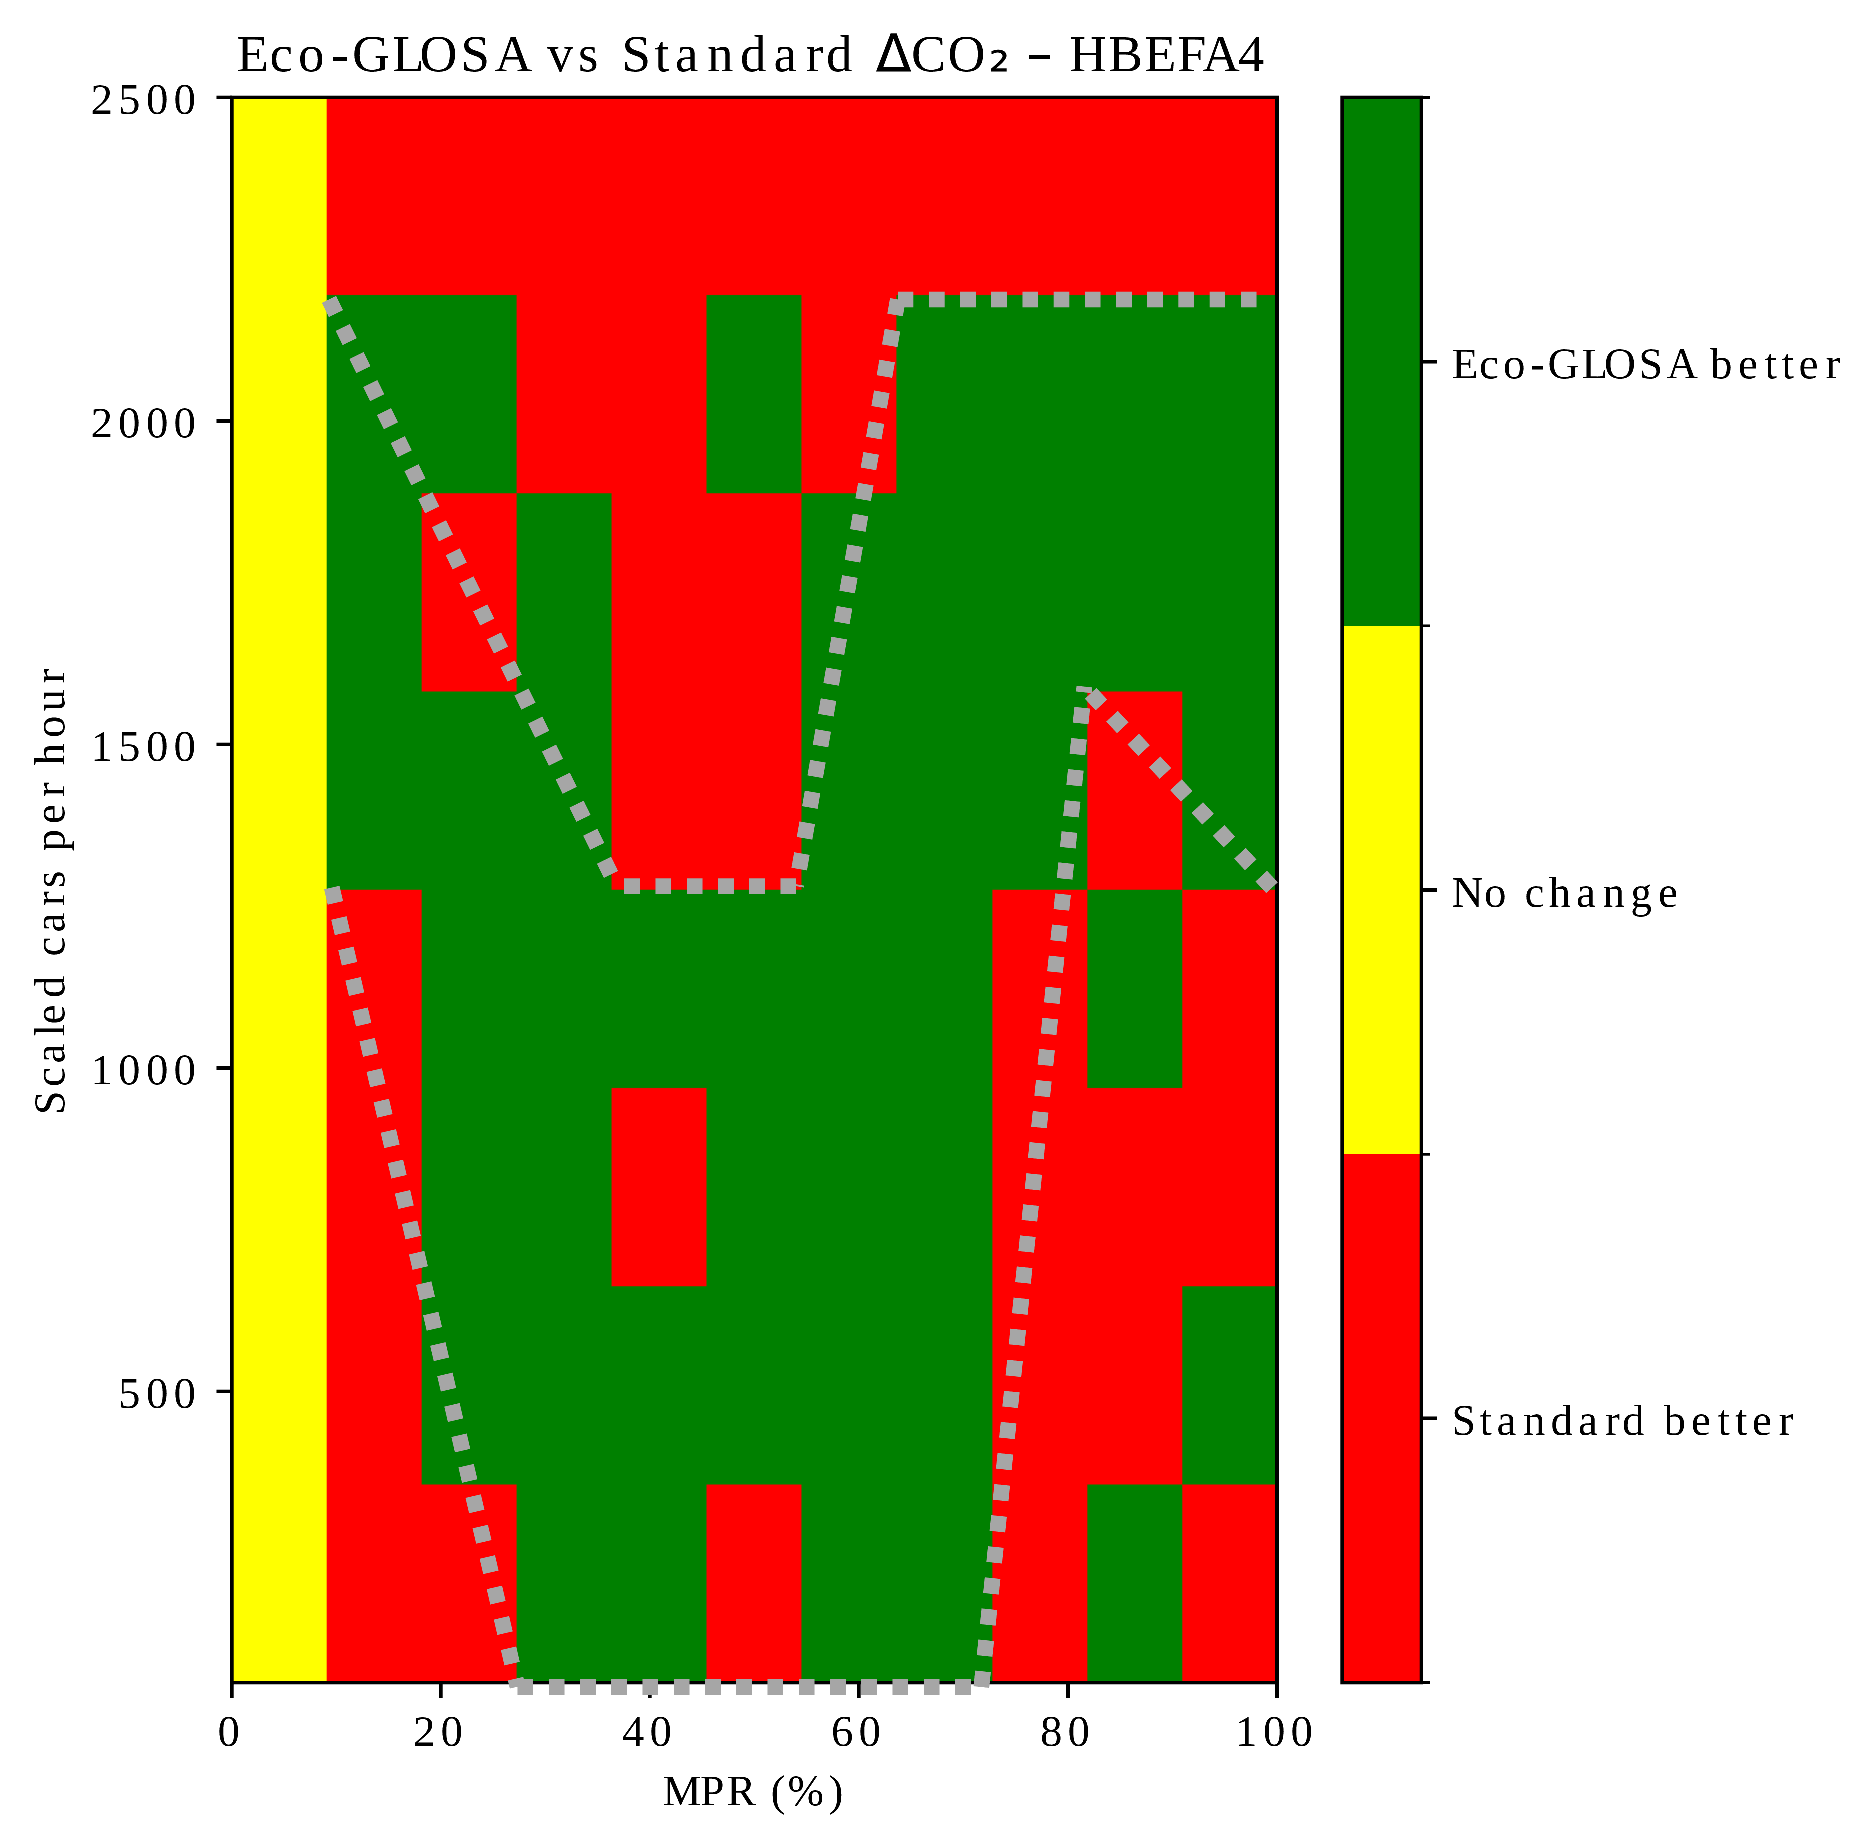
\includegraphics[width=\textwidth]{data/img/BreakEven/delta_CO2_HBEFA4.pdf}
    \caption{HBEFA4 model.}
    \label{fig:BE_EcoStd_HBEFA4}
  \end{subfigure}\hfill
  \begin{subfigure}[b]{0.45\textwidth}
    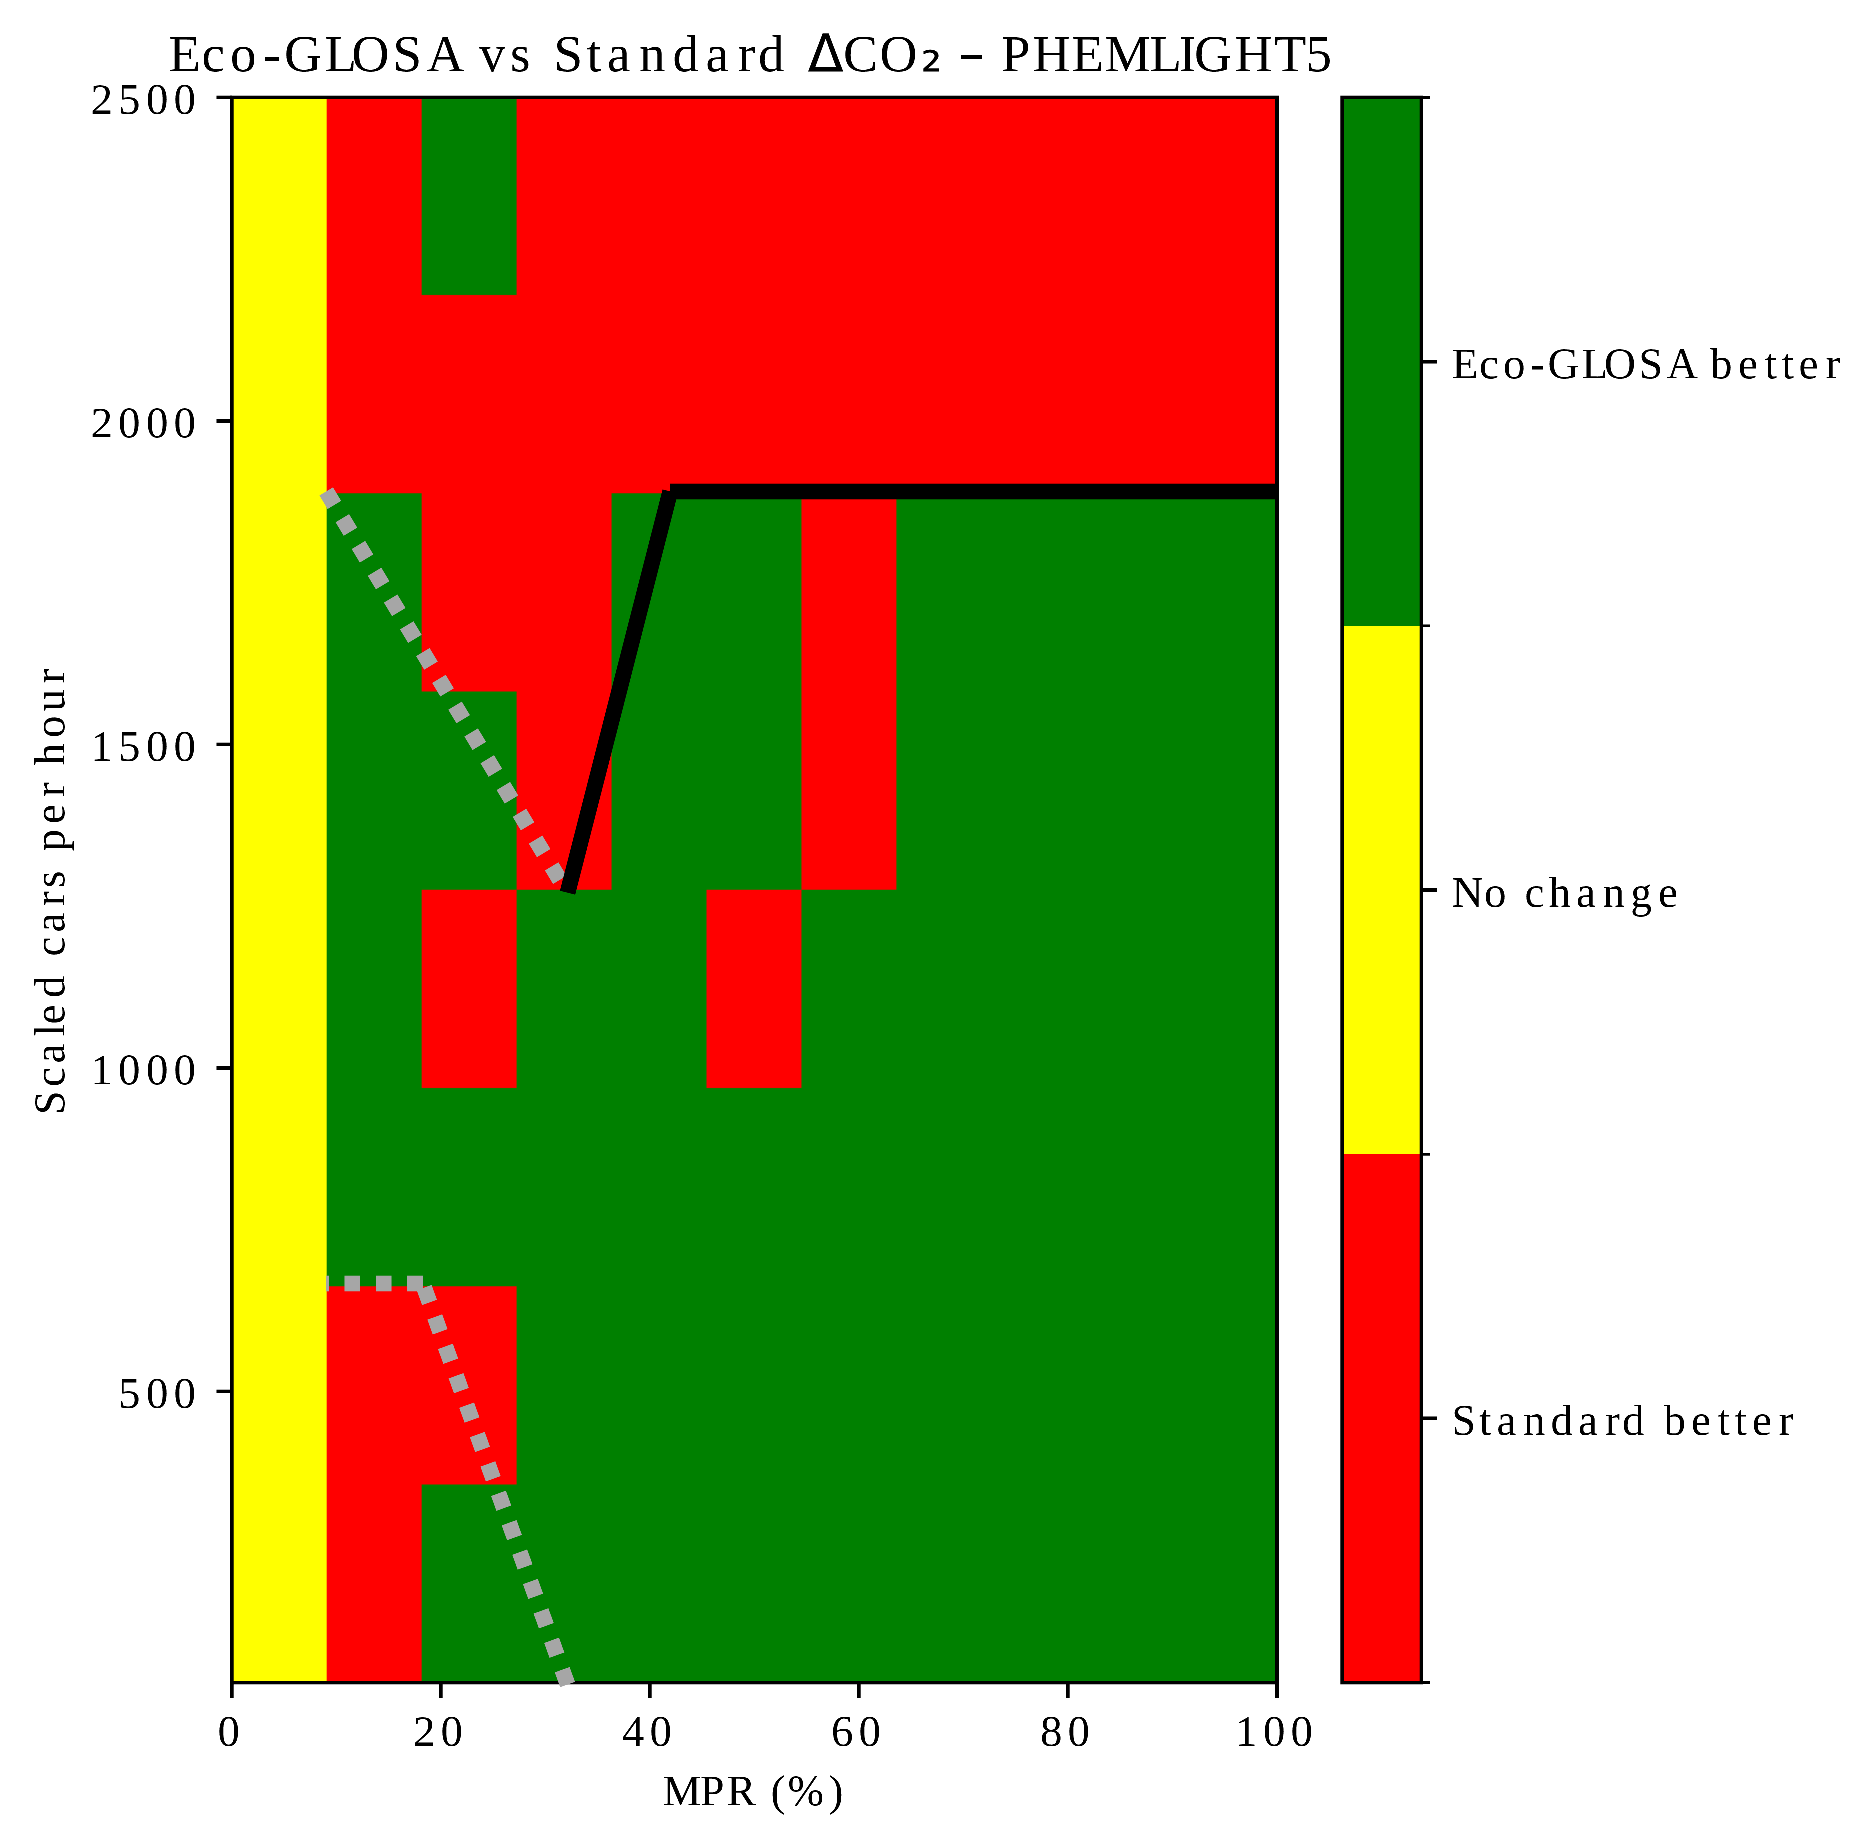
\includegraphics[width=\textwidth]{data/img/BreakEven/delta_CO2_PHEMLIGHT5.pdf}
    \caption{PHEMlight5 model.}
    \label{fig:BE_EcoStd_PHEM}
  \end{subfigure}
  \caption{Relative CO$_2$ emission reduction achieved by \ac{eco-glosa} compared to the Standard scenario (no \ac{glosa}). Green regions denote positive emission savings, while red regions indicate higher emissions relative to the Standard. Grey dashed envelopes delineate the empirically determined range in which \ac{eco-glosa} is effective; the solid black curve traces the optimal path of maximum emission reduction.}
  \label{fig:BE_EcoStd}
\end{figure}

\begin{table}[htb]
  \centering
  \caption{Break‐even analysis: CO$_2$ difference (g/km) between \ac{eco-glosa} and \ac{flow-glosa}. Positive values indicate \ac{eco-glosa} outperforms \ac{flow-glosa}.}
  \label{tab:BreakEven_EcoVsFlow}
  \resizebox{\textwidth}{!}{%
    \begin{tabular}{r l *{12}{r}}
      \toprule
      Cars & Fuel       & \textbf{0\% (Standard)} & 10\%    & 20\%    & 30\%      & 40\%      & 50\%     & 60\%       & 70\%    & 80\%    & 90\%    & 100\%   \\
      \midrule
      69   & HBEFA4     & \textbf{149.99}      & \textbf{0.53}   & \textbf{2.30}   & \textbf{0.68}   & \textbf{0.65}   & –3.55   & \textbf{1.63}    & –0.61  & –0.42  & –2.22  & –3.40  \\
      138  & HBEFA4     & \textbf{148.70}      & –6.45  & \textbf{0.26}   & \textbf{1.40}   & –4.20  & \textbf{1.84}  & –0.13   & –0.71  & –4.62  & 5.52   & 0.48   \\
      346  & HBEFA4     & \textbf{147.86}      & –1.66  & \textbf{2.19}   & –1.48  & –1.24  & \textbf{0.76}  & –0.22   & –1.16  & –2.95  & –1.48  & 0.35   \\
      692  & HBEFA4     & \textbf{148.06}      & \textbf{11.68}  & \textbf{1.07}   & \textbf{0.10}   & –0.98  & \textbf{1.02}  & –0.85   & –1.26  & –5.69  & –2.06  & –5.38  \\
      1385 & HBEFA4     & \textbf{149.86}      & \textbf{0.74}   & –0.39  & –0.71  & –1.84  & –0.37   & –2.18   & –2.01  & –0.66  & \textbf{0.97}   & –2.12  \\
      2077 & HBEFA4     & \textbf{152.91}      & \textbf{0.11}   & –2.97  & –2.38  & –0.79  & –4.25   & –3.62   & –2.82  & –1.65  & –1.73  & –4.13  \\
      2769 & HBEFA4     & \textbf{158.44}      & –5.23  & –1.99  & \textbf{–118.09} & –68.76 & –3.67   & \textbf{–272.42} & –4.30  & –3.51  & –2.69  & –3.91  \\
      3462 & HBEFA4     & \textbf{426.68}      & –54.38 & –88.56 & –102.44 & –134.41 & –157.82 & \textbf{–351.31} & –206.47 & –421.00 & –444.57 & –430.41 \\
      \midrule
      69   & PHEMlight5 & \textbf{155.51}      & –6.14  & –0.03  & \textbf{2.14}   & \textbf{2.65}   & \textbf{7.32}  & \textbf{1.26}    & \textbf{3.35}   & \textbf{1.32}   & \textbf{4.86}   & \textbf{16.51} \\
      138  & PHEMlight5 & \textbf{155.28}      & –4.94  & –2.09  & \textbf{3.63}   & \textbf{1.92}   & \textbf{4.39}  & \textbf{1.87}    & 0.51   & \textbf{6.64}   & \textbf{8.21}   & 2.86   \\
      346  & PHEMlight5 & \textbf{156.60}      & \textbf{8.46}   & \textbf{4.50}   & –0.15  & –2.59  & 0.13    & 0.39    & \textbf{1.46}   & \textbf{2.32}   & \textbf{6.19}   & 1.92   \\
      692  & PHEMlight5 & \textbf{157.36}      & 7.99   & –1.86  & –1.02  & –0.91  & –0.11   & \textbf{ –0.60} & –0.06  & \textbf{6.77}   & 1.69   & \textbf{4.51}  \\
      1385 & PHEMlight5 & \textbf{159.38}      & –1.46  & –3.82  & –4.83  & –4.89  & –4.80   & –6.19   & –3.65  & –5.33  & –0.86  & –1.36  \\
      2077 & PHEMlight5 & \textbf{162.83}      & –4.06  & –7.78  & –5.57  & –3.13  & –5.57   & –7.11   & –7.15  & –6.80  & –4.14  & –5.60  \\
      2769 & PHEMlight5 & \textbf{168.29}      & –30.19 & –69.10 & –138.25 & –125.33 & –148.94 & –172.00  & –189.98 & –142.67 & –167.68 & –104.93 \\
      3462 & PHEMlight5 & \textbf{344.88}      & –32.33 & –44.15 & –63.07  & –59.73  & –72.32  & –197.81  & –112.43 & –208.07 & –207.66 & –215.19 \\
      \bottomrule
    \end{tabular}%
  }
\end{table}

\begin{table}[htb]
  \centering
  \caption{Break‐even analysis: CO$_2$ difference (g/km) between \ac{eco-glosa} and Standard. Positive values indicate a reduction relative to the Standard.}
  \label{tab:BreakEven_EcoVsStd}
  \resizebox{\textwidth}{!}{%
    \begin{tabular}{r l *{12}{r}}
      \toprule
      Cars & Fuel       & \textbf{0\% (Standard)} & 10\%    & 20\%    & 30\%     & 40\%     & 50\%    & 60\%    & 70\%     & 80\%     & 90\%     & 100\%    \\
      \midrule
      69   & HBEFA4     & \textbf{149.99}      & –14.06 & –19.38 & \textbf{5.40}  & \textbf{22.11} & –15.56 & \textbf{6.54}  & \textbf{8.50}  & –4.29  & \textbf{2.17}  & –3.21  \\
      138  & HBEFA4     & \textbf{148.70}      & –9.72  & \textbf{5.89}  & \textbf{4.56}  & \textbf{6.55}  & \textbf{17.52} & \textbf{6.74}  & \textbf{8.11} & –13.27 & –14.47 & \textbf{2.02} \\
      346  & HBEFA4     & \textbf{147.86}      & –18.14 & \textbf{12.48} & \textbf{0.38}  & –5.30  & \textbf{16.25} & \textbf{4.94}  & \textbf{3.72} & –11.59 & –20.20 & –14.62 \\
      692  & HBEFA4     & \textbf{148.06}      & –20.25 & \textbf{1.82}  & \textbf{2.27}  & \textbf{8.91}  & \textbf{4.30}  & \textbf{5.07}  & \textbf{5.04} & –18.90 & \textbf{4.05}  & –13.03 \\
      1385 & HBEFA4     & \textbf{149.86}      & \textbf{11.98} & \textbf{8.69}  & \textbf{1.87}  & –0.86  & –3.83 & \textbf{4.40}  & \textbf{5.52} & \textbf{18.81} & –17.86 & \textbf{19.47} \\
      2077 & HBEFA4     & \textbf{152.91}      & \textbf{11.59} & –19.04 & \textbf{1.85}  & –5.16  & –4.66 & \textbf{5.54}  & \textbf{7.28} & \textbf{20.04} & \textbf{7.24}  & \textbf{19.61} \\
      2769 & HBEFA4     & \textbf{158.44}      & \textbf{8.76}  & \textbf{8.17}  & –112.49 & –65.49 & \textbf{14.37} & –260.65 & \textbf{9.24}  & \textbf{21.50} & \textbf{20.97} & \textbf{23.50} \\
      3462 & HBEFA4     & \textbf{426.68}      & –51.87 & –89.47 & –94.30  & –97.72 & –100.28 & –148.47 & –140.95 & –149.41 & –180.79 & –155.06 \\
      \midrule
      69   & PHEMlight5 & \textbf{155.51}      & –0.69  & \textbf{6.68}  & \textbf{7.14}  & \textbf{12.53} & \textbf{24.06} & \textbf{6.34}  & \textbf{10.97} & \textbf{17.26} & \textbf{19.01} & \textbf{17.94} \\
      138  & PHEMlight5 & \textbf{155.28}      & –0.40  & –7.12  & \textbf{5.37}  & \textbf{3.62}  & \textbf{11.02} & \textbf{6.47}  & \textbf{7.53}  & \textbf{5.15}  & \textbf{18.88} & \textbf{12.87} \\
      346  & PHEMlight5 & \textbf{156.60}      & \textbf{13.56} & \textbf{9.07}  & \textbf{0.79}  & \textbf{3.14}  & \textbf{8.81}  & \textbf{4.65}  & \textbf{5.37}  & \textbf{13.14} & \textbf{15.01} & \textbf{13.25} \\
      692  & PHEMlight5 & \textbf{157.36}      & \textbf{0.44}  & –9.96  & \textbf{0.16}  & \textbf{3.34}  & –5.65  & \textbf{3.85}  & \textbf{4.51}  & \textbf{13.50} & \textbf{13.52} & \textbf{18.50} \\
      1385 & PHEMlight5 & \textbf{159.38}      & \textbf{2.69}  & \textbf{0.52}  & –3.61 & \textbf{2.69}  & \textbf{1.37}  & –1.32  & \textbf{1.80}  & \textbf{5.31}  & \textbf{8.89}  & \textbf{11.17} \\
      2077 & PHEMlight5 & \textbf{162.83}      & \textbf{0.59}  & –2.37  & –3.25 & \textbf{0.84}  & \textbf{3.24}  & –0.05  & \textbf{0.80}  & \textbf{5.37}  & \textbf{10.65} & \textbf{8.52}  \\
      2769 & PHEMlight5 & \textbf{168.29}      & –23.10 & –63.72 & –135.11 & –115.95 & –137.81 & –163.38 & –179.44 & –127.66 & –153.08 & –87.61 \\
      3462 & PHEMlight5 & \textbf{344.88}      & –16.50 & \textbf{1.68}  & –54.31 & –12.24 & –24.62 & –63.75 & –65.57 & –20.02 & –14.53 & –22.90 \\
      \bottomrule
    \end{tabular}%
  }
\end{table}


\section{Computational Viability}
\label{sec:Results_Computational}

The computational viability of the \ac{eco-glosa} and \ac{flow-glosa} algorithms was assessed by measuring the total simulation runtime for each scenario. Because absolute execution times are hardware-dependent, this analysis focuses primarily on the relative computational overheads between different configurations. The raw durations are listed in Table~\vref{tab:CompViability_TraciComparison} and Table~\vref{tab:CompViability_SumoTraci}.
\mynewline
A primary finding is that the \ac{eco-glosa} algorithm is markedly slower than \ac{flow-glosa}, with the performance gap growing super-linearly with traffic volume, as documented in table~\vref{tab:CompViability_TraciComparison}. At a low demand of $69~\unit{\veh\per\hour}$, the controllers have nearly identical runtimes when no vehicles are equipped. However, at $100\%$ \ac{mpr} under the HBEFA4 model, the \ac{flow-glosa} simulation finishes in $154.27~\unit{\second}$, whereas \ac{eco-glosa} requires $282.56~\unit{\second}$, an increase of $83\%$. This disparity is accentuated by the more demanding PHEMlight5 model, where the slowdown factor reaches $6.2\times$ at full penetration. The performance gap becomes extreme in the saturated scenario of $3462~\unit{\veh\per\hour}$. Here, the \ac{eco-glosa} simulation is over $8.4\times$ slower with HBEFA4 and more than $32\times$ slower with PHEMlight5 compared to its \ac{flow-glosa} counterpart. This significant additional cost is attributable to the fuel-minimisation routine and the high-resolution engine-map lookups that the \ac{eco-glosa} controller must evaluate for every equipped vehicle at each simulation time step.
\mynewline
The choice of simulation interface also introduces a significant bottleneck. A comparison between running \ac{sumo} natively versus controlling it via the \ac{traci} client-server protocol reveals a substantial overhead caused by per-step socket communication (table~\vref{tab:CompViability_SumoTraci}. For a low-demand scenario ($69~\unit{\veh\per\hour}$), a \ac{traci}-controlled simulation takes up to nine times longer than a native \ac{sumo} run ($138.50~\unit{\second}$ versus $15.31~\unit{\second}$). In the saturated regime ($3462~\unit{\veh\per\hour}$), the penalty can be even higher. At $60\%$ \ac{mpr}, the \ac{traci} implementation requires $8613.54~\unit{\second}$, which is over $12\times$ longer than the $709.81~\unit{\second}$ needed for the native run. This demonstrates that the communication overhead of \ac{traci} is a major performance consideration, independent of the controller logic itself.
\mynewline
The graphical results in Figures~\vref{fig:Comp_69} to \vref{fig:Comp_3462} visually confirm these trends. At every demand level, the simulation time for \ac{eco-glosa} increases with a much steeper slope as a function of \ac{mpr} than that of \ac{flow-glosa}, which exhibits a milder, more manageable scaling.

\begin{figure}[htb]
  \centering
  \begin{subfigure}[b]{0.45\textwidth}
    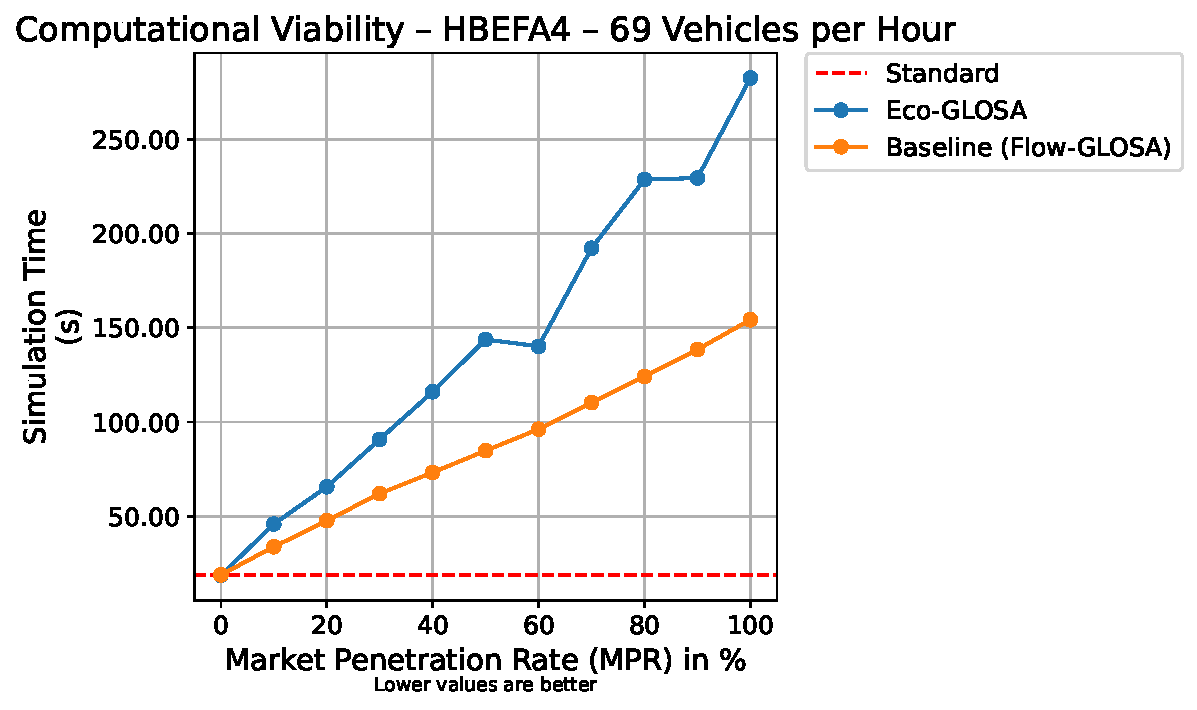
\includegraphics[width=\textwidth]{data/img/ComputationalViability/ComputationalViability_HBEFA4_Cars69.pdf}
    \caption{Runtimes with the HBEFA4 emission model.}
    \label{fig:Comp_69_HBEFA4}
  \end{subfigure}\hfill
  \begin{subfigure}[b]{0.45\textwidth}
    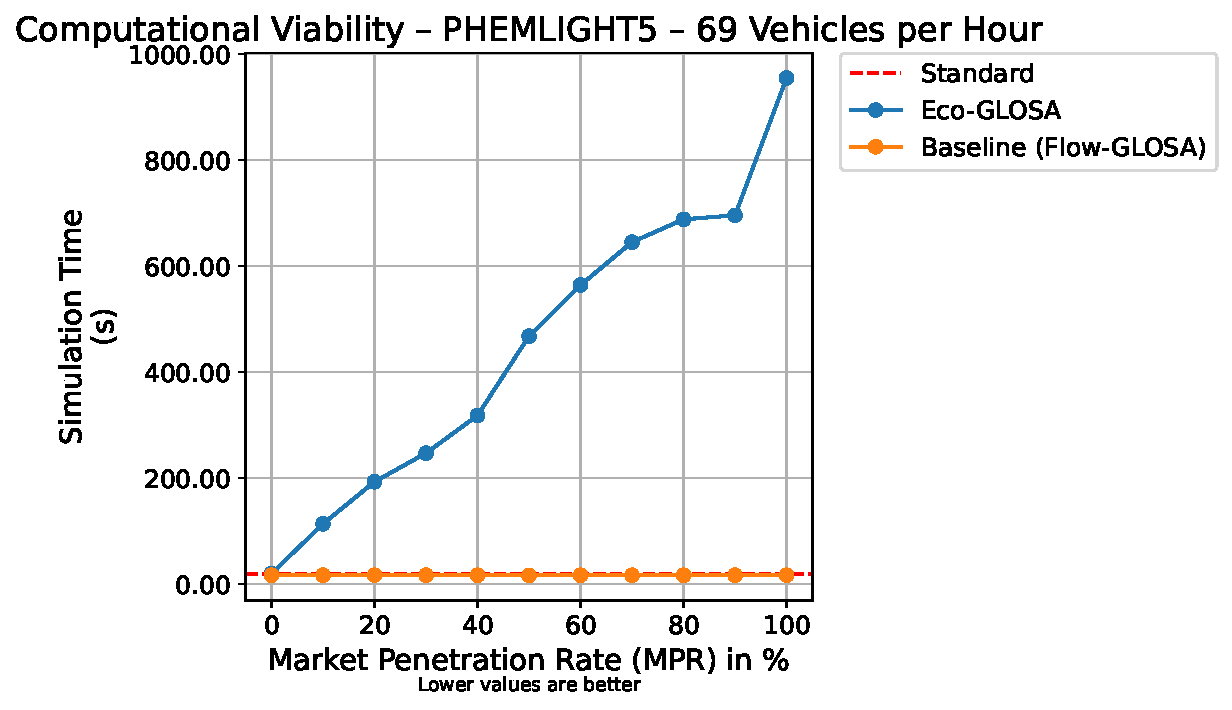
\includegraphics[width=\textwidth]{data/img/ComputationalViability/ComputationalViability_PHEMLIGHT5_Cars69.pdf}
    \caption{Runtimes with the PHEMlight5 emission model}
    \label{fig:Comp_69_PHEM}
  \end{subfigure}
  \caption[Computational Cost at Low Traffic Volume]{A comparison of simulation runtimes as a function of \ac{mpr} at a low traffic volume of $69~\unit{\veh\per\hour}$. The plots illustrate the computational cost for the Standard, \ac{eco-glosa}, and \ac{flow-glosa} controllers.}
  \label{fig:Comp_69}
\end{figure}

\begin{figure}[htb]
  \centering
  \begin{subfigure}[b]{0.45\textwidth}
    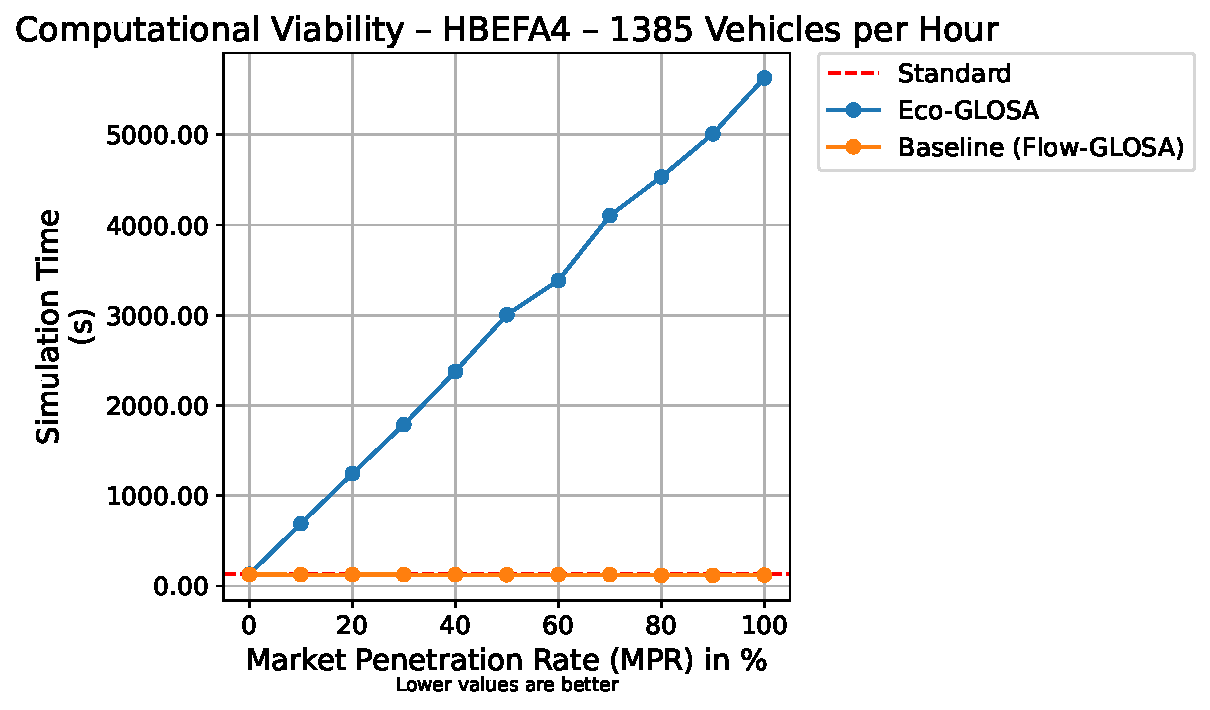
\includegraphics[width=\textwidth]{data/img/ComputationalViability/ComputationalViability_HBEFA4_Cars1385.pdf}
    \caption{Runtimes with the HBEFA4 emission model.}
    \label{fig:Comp_1385_HBEFA4}
  \end{subfigure}\hfill
  \begin{subfigure}[b]{0.45\textwidth}
    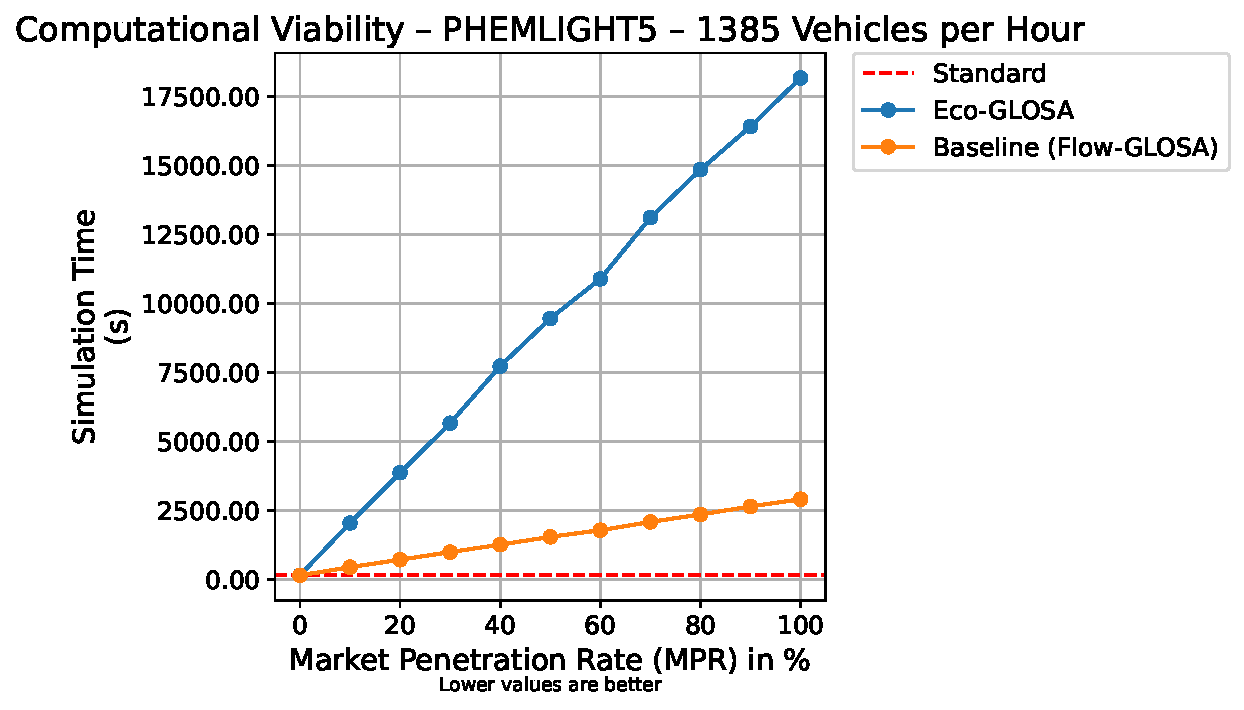
\includegraphics[width=\textwidth]{data/img/ComputationalViability/ComputationalViability_PHEMLIGHT5_Cars1385.pdf}
    \caption{Runtimes with the PHEMlight5 emission model.}
    \label{fig:Comp_1385_PHEM}
  \end{subfigure}
  \caption[Computational Cost at Intermediate Traffic Volume]{Simulation runtimes as a function of \ac{mpr} at an intermediate traffic volume of $1385~\unit{\veh\per\hour}$. The divergence in computational cost between \ac{eco-glosa} and \ac{flow-glosa} becomes more pronounced.}
  \label{fig:Comp_1385}
\end{figure}

\begin{figure}[htb]
  \centering
  \begin{subfigure}[b]{0.45\textwidth}
    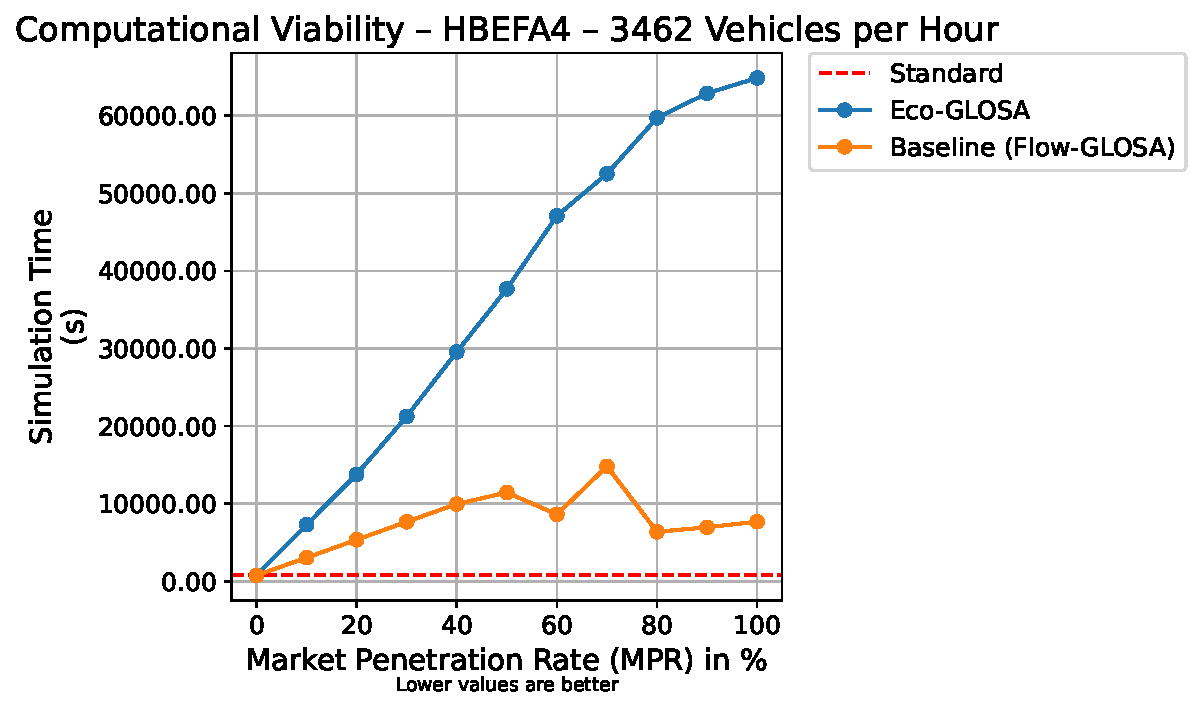
\includegraphics[width=\textwidth]{data/img/ComputationalViability/ComputationalViability_HBEFA4_Cars3462.pdf}
    \caption{Runtimes using the HBEFA4 model.}
    \label{fig:Comp_3462_HBEFA4}
  \end{subfigure}\hfill
  \begin{subfigure}[b]{0.45\textwidth}
    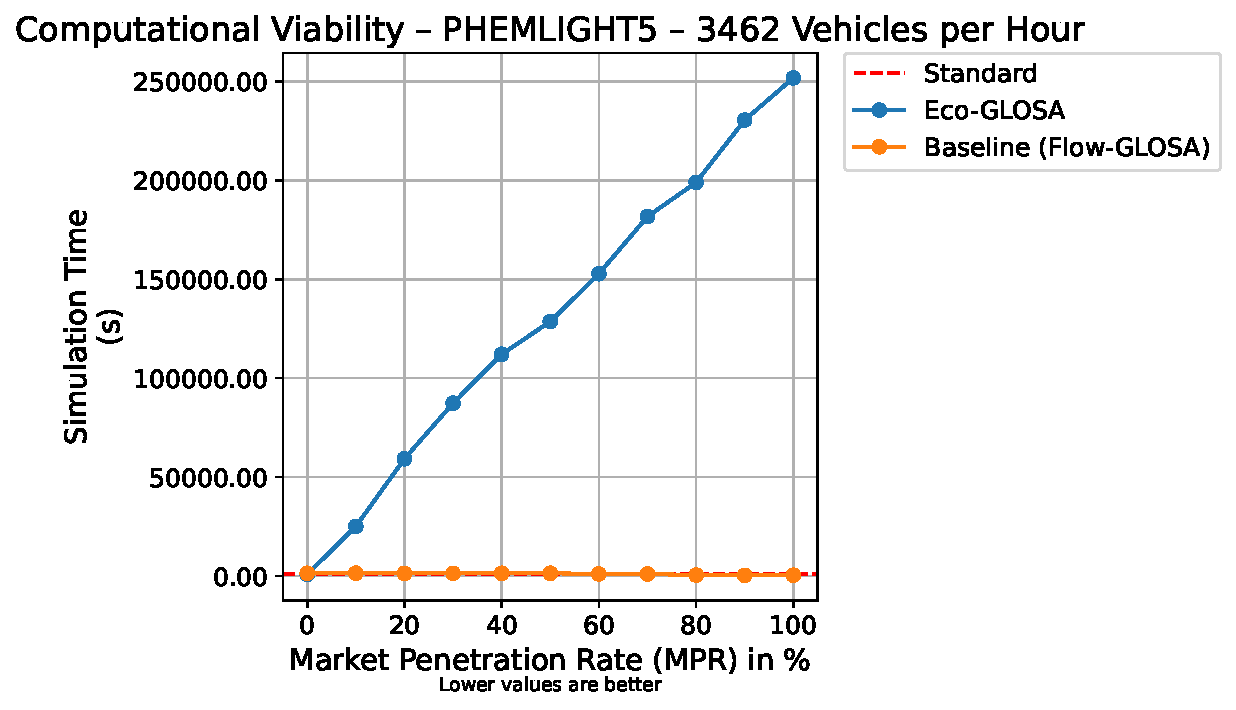
\includegraphics[width=\textwidth]{data/img/ComputationalViability/ComputationalViability_PHEMLIGHT5_Cars3462.pdf}
    \caption{Runtimes using the PHEMlight5 model}
    \label{fig:Comp_3462_PHEM}
  \end{subfigure}
  \caption[Computational Cost in Saturated Conditions]{Simulation runtimes versus \ac{mpr} in the fully saturated regime of $3462~\unit{\veh\per\hour}$. The plots highlight the extreme computational overhead of the \ac{eco-glosa} controller in high-density scenarios.}
  \label{fig:Comp_3462}
\end{figure}

\paragraph{Conclusion on Computational Cost.}
In summary, the \ac{eco-glosa} controller entails a steep computational surcharge, running up to $6\times$ slower than the baseline at low volumes and more than $32\times$ slower in full saturation. Furthermore, the \ac{traci} interface alone imposes an additional slowdown factor of $9\times$ to $12\times$ relative to a native implementation. These findings underline the necessity of using a native \ac{sumo} integration or a dedicated, GPU-accelerated implementation to achieve practical runtimes for complex \ac{eco-glosa} algorithms in large-scale or real-time deployments.

\begin{table}[htb]
  \centering
  \caption[Simulation Runtimes: Controller Comparison]{Absolute simulation runtimes (in seconds) for the \ac{eco-glosa} and \ac{flow-glosa} controllers under the \ac{traci} interface. The data is presented for all traffic volumes and both emission models. Note: absolute times are hardware-dependent.}
  \label{tab:CompViability_TraciComparison}
  \resizebox{\textwidth}{!}{%
    \begin{tabular}{l l l *{11}{c}}
      \toprule
      Vehicles & Algorithm                 & Fuel         & \textbf{0\% (Std.)} & 10\%       & 20\%       & 30\%       & 40\%       & 50\%       & 60\%       & 70\%       & 80\%       & 90\%       & 100\%      \\
      \midrule
      69.0  & Eco-GLOSA                  & HBEFA4       & \textbf{18.64}      & 45.85      & 65.61      & 90.83      & 116.07     & 143.79     & 140.17     & 192.22     & 228.63     & 229.47     & 282.56     \\
      69.0  & Baseline (Flow-GLOSA)      & HBEFA4       & \textbf{18.89}      & 33.81 & 47.66      & 62.03      & 73.24      & 84.78      & 96.20      & 110.26     & 124.18     & 138.50     & 154.27     \\
      69.0  & Eco-GLOSA                  & PHEMlight5   & \textbf{19.79}      & 113.47     & 192.99     & 246.83     & 318.11     & 467.78     & 564.11     & 645.15     & 688.17     & 695.72     & \textbf{954.95} \\
      69.0  & Baseline (Flow-GLOSA)      & PHEMlight5   & \textbf{19.74}      & 35.07      & 48.86      & 62.42      & 74.12      & 86.59      & 97.60      & 111.75     & 126.13     & 139.04     & 153.64     \\
      \midrule
      138.0 & Eco-GLOSA                  & HBEFA4       & \textbf{24.35}      & 71.47      & 109.07     & 147.94     & 199.01     & 276.45     & 271.03     & 374.97     & 429.04     & 476.37     & 538.66     \\
      138.0 & Baseline (Flow-GLOSA)      & HBEFA4       & \textbf{24.51}      & 52.91 & 78.94      & 101.98     & 133.92     & 160.74     & 183.96     & 216.30     & 243.30     & 272.53     & 296.83     \\
      138.0 & Eco-GLOSA                  & PHEMlight5   & \textbf{26.35}      & 167.41     & 324.63     & 393.20     & 508.62     & 859.65     & 808.66     & 1041.76    & 1225.48    & 1519.14    & \textbf{1617.62} \\
      138.0 & Baseline (Flow-GLOSA)      & PHEMlight5   & \textbf{26.35}      & 55.08      & 81.36      & 104.24     & 136.92     & 164.67     & 186.48     & 218.25     & 249.58     & 275.22     & 299.86     \\
      \midrule
      346.0 & Eco-GLOSA                  & HBEFA4       & \textbf{41.48}      & 157.89     & 280.45     & 464.09     & 539.94     & 709.78     & 802.68     & 933.80     & 1062.64    & 1178.17    & 1337.18    \\
      346.0 & Baseline (Flow-GLOSA)      & HBEFA4       & \textbf{41.25}      & 108.99 & 179.65     & 253.48     & 309.06     & 382.80     & 449.63     & 510.24     & 581.60     & 654.66     & 697.96     \\
      346.0 & Eco-GLOSA                  & PHEMlight5   & \textbf{45.96}      & 408.26     & 909.13     & 1422.53    & 1636.71    & 2058.14    & 2573.80    & 2762.42    & 3290.75    & 3709.17    & \textbf{4034.62} \\
      346.0 & Baseline (Flow-GLOSA)      & PHEMlight5   & \textbf{45.96}      & 113.87     & 183.71     & 257.67     & 314.50     & 384.77     & 449.25     & 522.51     & 583.57     & 653.83     & 702.11     \\
      \midrule
      692.0 & Eco-GLOSA                  & HBEFA4       & \textbf{70.06}      & 290.22     & 507.57     & 824.96     & 1077.34    & 1316.33    & 1604.01    & 1844.68    & 2081.46    & 2413.43    & 2689.71    \\
      692.0 & Baseline (Flow-GLOSA)      & HBEFA4       & \textbf{70.01}      & 199.61 & 328.83     & 466.43     & 598.32     & 746.09     & 878.61     & 1009.32    & 1138.79    & 1285.82    & 1423.82    \\
      692.0 & Eco-GLOSA                  & PHEMlight5   & \textbf{79.38}      & 830.27     & 1458.45    & 2363.30    & 3059.37    & 3879.64    & 4721.61    & 5316.79    & 6342.07    & 7676.13    & \textbf{8407.14} \\
      692.0 & Baseline (Flow-GLOSA)      & PHEMlight5   & \textbf{78.96}      & 207.93     & 339.90     & 475.03     & 608.61     & 761.29     & 905.29     & 1024.79    & 1159.32    & 1286.28    & 1435.04    \\
      \midrule
      1385.0& Eco-GLOSA                  & HBEFA4       & \textbf{129.28}     & 690.08     & 1243.97    & 1788.03    & 2377.18    & 3004.73    & 3385.14    & 4103.90    & 4533.56    & 5010.08    & 5629.95    \\
      1385.0& Baseline (Flow-GLOSA)      & HBEFA4       & \textbf{129.45}     & 429.51 & 708.63     & 967.43     & 1238.00    & 1535.47    & 1790.18    & 2092.41    & 2322.02    & 2641.07    & 2872.80    \\
      1385.0& Eco-GLOSA                  & PHEMlight5   & \textbf{149.43}     & 2044.34    & 3869.10    & 5660.32    & 7731.41    & 9458.66    & 10890.27   & 13110.24   & 14853.12   & 16414.57   & \textbf{18175.02} \\
      1385.0& Baseline (Flow-GLOSA)      & PHEMlight5   & \textbf{147.99}     & 443.74     & 714.95     & 990.27     & 1261.04    & 1543.80    & 1784.86    & 2084.13    & 2356.39    & 2643.55    & 2908.28    \\
      \midrule
      2077.0& Eco-GLOSA                  & HBEFA4       & \textbf{194.76}     & 1059.69    & 1975.94    & 2762.06    & 3673.14    & 4655.86    & 5286.35    & 6359.72    & 7099.10    & 8021.73    & 8871.25    \\
      2077.0& Baseline (Flow-GLOSA)      & HBEFA4       & \textbf{192.60}     & 627.27 & 1045.43    & 1477.00    & 1903.69    & 2327.89    & 2743.54    & 3146.68    & 3573.26    & 3965.27    & 4393.02    \\
      2077.0& Eco-GLOSA                  & PHEMlight5   & \textbf{226.03}     & 2940.59    & 5345.12    & 8709.82    & 12229.50   & 14562.74   & 17021.70   & 19812.39   & 22670.23   & 24838.64   & \textbf{27842.28} \\
      2077.0& Baseline (Flow-GLOSA)      & PHEMlight5   & \textbf{222.82}     & 652.90     & 1077.84    & 1530.54    & 1937.15    & 2392.21    & 2784.75    & 3172.89    & 3612.89    & 4026.18    & 4391.33    \\
      \midrule
      2769.0& Eco-GLOSA                  & HBEFA4       & \textbf{265.40}     & 1717.59    & 3066.87    & 9783.80 & 9676.92    & 6817.65    & 29119.22 & 9456.50    & 10410.82   & 11515.24   & 12838.56   \\
      2769.0& Baseline (Flow-GLOSA)      & HBEFA4       & \textbf{263.91}     & 911.38     & 1502.86    & 2086.31    & 2665.99    & 3275.49    & 3829.42    & 4361.18    & 4926.63    & 5492.37    & 5976.06    \\
      2769.0& Eco-GLOSA                  & PHEMlight5   & \textbf{306.78}     & 5033.51    & 18916.38   & 47755.69   & 69552.51   & 94654.61   & 114831.96  & 145268.05  & 142126.60  & 165711.80  & \textbf{139171.65} \\
      2769.0& Baseline (Flow-GLOSA)      & PHEMlight5   & \textbf{305.10}     & 944.66     & 1549.56    & 2131.41    & 2691.56    & 3273.49    & 3865.19    & 4369.02    & 4948.13    & 5467.45    & 6036.59    \\
      \midrule
      3462.0& Eco-GLOSA                  & HBEFA4       & \textbf{762.47}     & 7291.92    & 13774.00   & 21248.52   & 29553.07   & 37682.93   & 47089.12   & 52511.10   & 59711.69   & 62882.26   & 64860.61   \\
      3462.0& Baseline (Flow-GLOSA)      & HBEFA4       & \textbf{753.90}     & 3029.19 & 5342.64    & 7660.62    & 9947.82    & 11430.39   & 8613.54    & 14805.14   & 6367.47    & 6947.72    & 7670.32    \\
      3462.0& Eco-GLOSA                  & PHEMlight5   & \textbf{867.03}     & 25083.58   & 59247.59   & 87348.07   & 112061.03  & 128604.77  & 152756.97  & 181628.56  & 198892.38  & 230399.98  & \textbf{251661.36} \\
      3462.0& Baseline (Flow-GLOSA)      & PHEMlight5   & \textbf{858.37}     & 3133.66    & 5465.48    & 7801.65    & 9987.87    & 11538.38   & 8697.48    & 14902.05   & 6354.86    & 7020.78    & 7713.73    \\
      \bottomrule
    \end{tabular}%
  }
\end{table}

\begin{table}[htb]
  \centering
  \caption[Simulation Runtimes: Native SUMO vs. TraCI]{Comparison of simulation runtimes (in seconds) between a native \ac{sumo} implementation and the \ac{traci} interface for the \ac{flow-glosa} controller. The data illustrates the computational overhead introduced by the external interface.}
  \label{tab:CompViability_SumoTraci}
  \resizebox{\textwidth}{!}{%
    \begin{tabular}{l l l *{11}{c}}
      \toprule
      Cars & Interface    & Fuel         & \textbf{0\% (Std.)} & 10\%       & 20\%       & 30\%       & 40\%       & 50\%       & 60\%       & 70\%       & 80\%       & 90\%       & 100\%      \\
      \midrule
      69.0  & \ac{sumo}     & HBEFA4       & \textbf{15.51}      & 15.38      & 15.64      & 15.55      & 15.52      & 15.79      & 15.15      & 15.41      & 15.52      & 15.31      & \textbf{15.20}      \\
      69.0  & \ac{traci}    & HBEFA4       & \textbf{18.89}      & \textbf{33.81} & 47.66      & 62.03      & 73.24      & 84.78      & 96.20      & 110.26     & 124.18     & 138.50     & \textbf{154.27}     \\
      69.0  & \ac{sumo}     & PHEMlight5   & \textbf{16.47}      & 16.34      & 16.41      & 16.61      & 16.47      & 15.98      & 16.39      & 16.24      & 16.37      & 16.37      & \textbf{16.42}      \\
      69.0  & \ac{traci}    & PHEMlight5   & \textbf{19.74}      & \textbf{35.07} & 48.86      & 62.42      & 74.12      & 86.59      & 97.60      & 111.75     & 126.13     & 139.04     & \textbf{153.64}     \\
      \midrule
      3462.0& \ac{sumo}     & HBEFA4       & \textbf{732.46}     & 738.94     & 744.20     & 696.91     & 713.94     & 729.21     & 709.81     & 686.57     & 739.10     & 725.49     & \textbf{727.38}     \\
      3462.0& \ac{traci}    & HBEFA4       & \textbf{753.90}     & \textbf{3029.19} & 5342.64    & 7660.62    & 9947.82    & 11430.39   & 8613.54    & 14805.14   & 6367.47    & 6947.72    & \textbf{7670.32}    \\
      3462.0& \ac{sumo}     & PHEMlight5   & \textbf{834.27}     & 842.27     & 848.58     & 792.96     & 819.15     & 832.40     & 815.79     & 785.65     & 846.47     & 835.91     & \textbf{831.79}     \\
      3462.0& \ac{traci}    & PHEMlight5   & \textbf{858.37}     & \textbf{3133.66} & 5465.48    & 7801.65    & 9987.87    & 11538.38   & 8697.48    & 14902.05   & 6354.86    & 7020.78    & \textbf{7713.73}    \\
      \bottomrule
    \end{tabular}%
  }
\end{table}

\section{Discussion}
\label{sec:Results_Discussion}

This discussion synthesises the extensive observations from the simulation campaign, providing a holistic interpretation of the empirical results. The primary goal is to address the three research questions articulated in Section~\vref{sec:Proposed_Eco_Driving_GLOSA_Algorithm} by integrating quantitative findings from the performance metrics with qualitative insights from trajectory-level analyses. By examining the performance of the \ac{eco-glosa} controller against both the Standard (uncontrolled) and \ac{flow-glosa} benchmarks, it is possible to delineate the precise operating conditions under which each strategy is most effective. The central narrative emerging from this analysis is that of a fundamental trade-off between vehicle-level eco-efficiency and network-level traffic stability, a dichotomy whose balance is critically dependent on traffic density and technology penetration.

\subsection*{Addressing Research Question 1: Fuel Efficiency}
The first research question sought to quantify the extent to which the \ac{eco-glosa} algorithm reduces fuel consumption. The findings reveal a stark, bimodal performance profile that is highly sensitive to traffic density.
\mynewline
In under-saturated conditions, \ac{eco-glosa} consistently and significantly reduces per-vehicle fuel consumption. Under light demand ($q=69~\unit{\veh\per\hour}$), for instance, the mean \ac{co2} emissions are reduced by a substantial $15.5\%$ relative to Standard driving. This considerable saving originates directly from the \ac{dp} controller's core logic, which actively suppresses high-power transient states. The optimal trajectory prescribed by the algorithm effectively shifts necessary acceleration phases into the engine's most efficient operating band and, most importantly, avoids energy-intensive stop-start cycles by timing the arrival at the intersection with the green phase. This benefit persists up to moderate demand levels, where at $q=692~\unit{\veh\per\hour}$, fuel usage is still diminished by a notable $11.8\%$ at full penetration under the PHEMlight5 model.
\mynewline
However, this paradigm of efficiency dramatically inverts as traffic density surpasses a critical threshold. At higher demand levels ($\gls{q} > 1385~\unit{\veh\per\hour}$), the \ac{eco-glosa} strategy becomes counterproductive. The controller, in its myopic pursuit of an optimal energy profile for the individual vehicle, frequently revises its speed advisories in response to emergent queueing dynamics. This leads to oscillatory speed profiles and repeated, inefficient re-accelerations. At a demand of $2769~\unit{\veh\per\hour}$ and $30\%$ penetration, the strategy increases \ac{co2} emissions by over $35~\unit{\gram\per\kilo\metre}$ compared to the Standard scenario (under PHEMlight5). Trajectory plots reveal the cause: equipped vehicles repeatedly accelerate to catch a green window, only to brake hard due to the slower, non-equipped vehicle queue ahead.
\mynewline
This behaviour means that the break-even penetration rate, $\gls{p}^\star$, at which \ac{eco-glosa} becomes beneficial, shifts upwards with demand. As shown in Figure~\vref{fig:BE_EcoFlow}, for flows below $700~\unit{\veh\per\hour}$, a penetration of just $\gls{p}^\star\approx30\%$ is often sufficient. In contrast, at flows approaching $2000~\unit{\veh\per\hour}$, the required penetration rises to $\gls{p}^\star > 80\%$. Furthermore, the choice of emission model sensitises these trends. The physics-based PHEMlight5 model predicts a narrower region of net benefit for \ac{eco-glosa} than the polynomial HBEFA4 model, as it more accurately penalises the transient events induced by the controller in dense traffic. This underscores the need for back-end models that faithfully represent real-world powertrain dynamics.

\subsection*{Addressing Research Question 2: Traffic-Flow Effects}
The second research question addressed the impact of the \ac{eco-glosa} controller on network-level traffic performance. The evidence unequivocally demonstrates that the \ac{flow-glosa} controller systematically outperforms both the eco-variant and the no-GLOSA Standard in terms of network throughput and kinematic smoothness, especially when it matters most: in congested conditions.
\mynewline
This divergence is most apparent under heavy demand. At $2769~\unit{\veh\per\hour}$ and a high penetration rate of $90\%$, the \ac{flow-glosa} controller successfully maintains traffic flow, achieving a high average speed of $12.46~\unit{\metre\per\second}$ while virtually eliminating stops, reducing them to just $0.07~\unit{\stops\per\veh}$. In stark contrast, under the same conditions, the \ac{eco-glosa} strategy induces a severe traffic jam. Its average speed collapses to just $2.57~\unit{\metre\per\second}$, and the stop frequency explodes to over $23~\unit{\stops\per\veh}$ (under the PHEMlight5 model).
\mynewline
The fundamental cause of this divergence lies in the objective mismatch between the controllers. The cost function for the \ac{eco-glosa} controller meticulously prioritises the vehicle's fuel consumption, penalising deviation from a calculated optimal speed. Crucially, it omits any term related to network throughput or queue length. Consequently, the optimiser often schedules extended slack times to allow for slower, more gradual approaches. While beneficial for a single vehicle in a vacuum, this behaviour in dense traffic creates voids in the traffic stream, inadvertently promoting queue growth and forcing following vehicles to brake.
\mynewline
The acceleration and jerk metrics, which serve as proxies for driving comfort, mirror this divergence. At a moderate demand of $692~\unit{\veh\per\hour}$, the eco-guidance successfully reduces mean acceleration by $12\%$ compared to standard driving. However, the frequent speed revisions in denser traffic can increase mean jerk by up to $8\%$, indicating a less smooth ride. Conversely, \ac{flow-glosa} smooths both acceleration and jerk profiles once penetration exceeds $60\%$, as it encourages vehicles to form stable platoons that traverse the green window at a near-constant speed. This is a direct result of its singular focus on maintaining traffic momentum.
\mynewline
Finally, green‐phase utilisation further highlights the trade‐offs. At low flows, \ac{eco-glosa} can achieve higher per‐vehicle green‐time utilisation ratios as individual vehicles glide more slowly across the intersection. From a network perspective, however, this comes at the expense of overall capacity. At demand levels above $1500~\unit{\veh\per\hour}$, the number of vehicles dispatched per green phase under \ac{eco-glosa} declines relative to both the Standard and \ac{flow-glosa} benchmarks, for example, under PHEMlight5 at $2769~\unit{\veh\per\hour}$ dispatch falls from $46.03$ to $37.83$ vehicles ($–17.9\%$), as confirmed in Table~\vref{tab:GreenPhaseFlow}. In contrast, the \ac{flow-glosa} baseline curves not only preserve but enhance throughput at full penetration, increasing dispatch by up to $17.5\%$ at $3462~\unit{\veh\per\hour}$ (from $49.03$ to $57.60$ vehicles) by design, demonstrating superior green‐phase capacity under heavy demand.

\subsection*{Addressing Research Question 3: Critical Thresholds and Operating Regimes}
The third research question sought to identify the critical thresholds where the benefits and drawbacks of each controller strategy become significant. By synthesising the full suite of performance metrics, including emissions, throughput, speed, and stop frequency, the analysis defines three distinct operating regimes. The optimal controller choice depends critically on these regimes, which are a function of traffic density ($\gls{q}$) and market penetration rate ($\gls{p}$).

\paragraph{The Under-Saturated Regime ($\gls{q} < 700~\unit{\veh\per\hour}$)}
In low-density traffic, \textit{\ac{eco-glosa} is the superior strategy for improving fuel efficiency}. The analysis of the PHEMlight5 model, considered the more physically accurate, shows that \ac{eco-glosa} consistently outperforms both the Standard and \ac{flow-glosa} scenarios once penetration surpasses a modest $30\%$ \ac{mpr}. It achieves a peak \ac{co2} reduction of $+24.06~\unit{\gram\per\kilo\metre}$ compared to an uncontrolled vehicle. The HBEFA4 model also shows benefits, though its predictions are more volatile. Crucially, in this regime, the application of \ac{eco-glosa} does not negatively impact key traffic flow metrics; average speeds and throughput are maintained. This makes it a low-risk, high-reward strategy in light traffic conditions.

\paragraph{The Transition Regime ($700 \le q \le 2300~\unit{\veh\per\hour}$)}
This intermediate range represents a critical and unstable \enquote{tipping point} where \textit{\ac{flow-glosa} becomes the more robust and reliable choice}. The myopic, fuel-saving logic of the \ac{eco-glosa} controller becomes a significant liability here. As seen with the PHEMlight5 model, its attempts to advise slower speeds can actively induce a traffic jam where none existed, causing average speeds to collapse and emissions to increase by as much as $163.38~\unit{\gram\per\kilo\metre}$ compared to the Standard case. The break-even analysis further reveals that the required penetration for \ac{eco-glosa} to outperform \ac{flow-glosa} skyrockets from $30\%$ to over $80\%$ as density increases through this regime. Given the severe emission penalties associated with failure, deploying \ac{eco-glosa} is only advisable if near-universal adoption can be guaranteed.

\paragraph{The Saturated Regime ($q > 2300~\unit{\veh\per\hour}$)}
In heavy and over-saturated traffic, \textit{\ac{flow-glosa} is unequivocally the dominant and only effective strategy}. The primary challenge in this regime is not optimising fuel efficiency but preventing total network collapse. The \ac{eco-glosa} controller consistently exacerbates congestion, increasing \ac{co2} emissions by over $50\%$ and accumulating more than $35~\unit{\stops\per\veh}$. In stark contrast, \ac{flow-glosa}, at a penetration of $80\%$ or higher, actively dissolves traffic jams. This intervention restores free-flow speeds and, by eliminating highly inefficient stop-start cycles, delivers profound \ac{co2} reductions of up to $64\%$. In this regime, maximising throughput is the most effective ecological strategy.

\paragraph{Final Answer to Research Question 3}
In conclusion, there is no single superior controller; the optimal strategy is dictated by the real-time traffic state. The critical thresholds are not fixed points but rather dynamic boundaries between three core operating regimes. For demands below approximately $700~\unit{\veh\per\hour}$, \ac{eco-glosa} can be safely deployed to achieve moderate energy savings. For demands above $2300~\unit{\veh\per\hour}$, \ac{flow-glosa} is essential for resolving gridlock and yielding the largest environmental co-benefits. In the wide and volatile transition range between these thresholds, the risk of \ac{eco-glosa} inducing congestion makes the throughput-focused \ac{flow-glosa} the most prudent and reliable choice for deployment.

\subsection*{Supplementary Observations and Practical Considerations}
Beyond the primary performance metrics, two practical considerations emerge from the analysis: the substantial computational burden of the \ac{eco-glosa} controller and the critical influence of the chosen emission model on the results.
\mynewline
First, the computational cost of the \ac{eco-glosa} optimiser is significant. In the most demanding scenario of $3462~\unit{\veh\per\hour}$ with full penetration, a simulation run under the PHEMlight5 model requires over $250,000~\unit{\second}$ of computation time. This is more than $32$ times longer than the $7,714~\unit{\second}$ needed for the simpler \ac{flow-glosa} logic under the same conditions (Table~\vref{tab:CompViability_TraciComparison}). This massive overhead, which scales with the number of advisory updates and engine-map lookups, indicates that real-world, online deployment of such a detailed optimisation algorithm would necessitate either dedicated hardware acceleration or the use of computationally cheaper surrogate models to approximate the fuel consumption function.
\mynewline
Second, the choice of emission back-end model critically influences the strategic conclusions that can be drawn. The high-fidelity PHEMlight5 model reveals a well-defined, albeit smaller, operational window where the \ac{eco-glosa} controller is beneficial. As seen in the break-even charts (Figure~\vref{fig:BE_EcoFlow_PHEM}), its performance boundaries are clear, providing a predictable understanding of where the strategy succeeds and where it fails. By comparison, the performance map generated by the HBEFA4 model is extremely unstable and fragmented (Figure~\vref{fig:BE_EcoFlow_HBEFA4}). Its relative insensitivity to transient driving states results in an unpredictable mix of benefits and penalties, which makes a clear and confident evaluation of the controller's effectiveness far more challenging. This underscores a key methodological insight: for developing and assessing advanced control strategies, a physics-based model like PHEMlight5 is invaluable. While it may reveal a more constrained operating range, the clarity and predictability it provides are essential for defining reliable deployment guidelines.

\subsection*{Limitations of the Study}
For academic rigour, it is essential to acknowledge the limitations of this work. The findings should be interpreted in the context of the following methodological constraints:
\begin{itemize}
    \item \textbf{Network Scope:} The analysis is confined to a single, isolated intersection corridor with a length of $1.2~\unit{\kilo\metre}$. Consequently, network-level phenomena such as multi-junction signal coordination and queue spill-back from downstream bottlenecks are not modelled.

    \item \textbf{Fleet Homogeneity:} The study assumes a homogenous powertrain fleet. It does not capture the complex dynamic and emission interactions that would occur in a mixed fleet of passenger cars, heavy-duty vehicles, and hybrid or electric vehicles.

    \item \textbf{Ideal Communications:} An ideal \ac{v2i} communication channel is assumed, with no modelling of real-world factors such as data latency, packet loss, or communication range limitations, which could affect controller performance.

    \item \textbf{Driver Compliance:} The model presupposes that all drivers comply perfectly with the issued advisories. Real-world driver behaviour would likely involve probabilistic compliance, which would effectively alter the operational market penetration rate.

    \item \textbf{Static Signal Control:} The analysis is based on a static, fixed-time signal plan. The results may differ in corridors that employ modern adaptive traffic signal control systems, which dynamically adjust phasing in response to traffic demand.
\end{itemize}

\subsection*{Conclusion}
In aggregate, this research provides a nuanced and data-driven answer to the question of how to best leverage \ac{glosa} systems for environmental and traffic benefits. The primary conclusion is that a \enquote{one-size-fits-all} approach is suboptimal. The optimal controller strategy is not fixed but is instead a function of the real-time traffic state, with a clear trade-off emerging between vehicle-level eco-efficiency and network-level stability.
\mynewline
The \ac{eco-glosa} strategy demonstrates this trade-off clearly. It yields robust fuel savings of up to $15.5\%$ in low-density conditions by smoothing driving profiles and avoiding unnecessary stops. However, its effectiveness erodes rapidly with increasing demand. The controller's myopic focus on per-vehicle optimisation induces system-level instabilities, leading to increased congestion and, paradoxically, a surge in emissions by over $160\%$ in some scenarios. In contrast, the \ac{flow-glosa} strategy, by synchronising vehicle platoons, proves to be a powerful tool for suppressing queue growth and restoring free-flow conditions. In doing so, it delivers profound emission reductions of up to $64\%$ in saturated regimes, demonstrating that in congested cities, the most effective green driving strategy is one that keeps traffic moving. These performance characteristics are framed by practical considerations, including the substantial computational overhead of the \ac{eco-glosa} algorithm, which can be over $30\times$ slower than \ac{flow-glosa}, and the critical influence of the emission model, where the higher fidelity of PHEMlight5 is essential for accurately revealing the controller's failure modes in congestion.
\mynewline
In direct answer to the research questions, this thesis finds that: \textit{\vref{rq1}} --- the \ac{eco-glosa} controller's impact on fuel efficiency is dichotomous, offering modest savings in light traffic but causing severe penalties in congestion; \textit{\vref{rq2}} --- the \ac{eco-glosa} controller severely degrades network performance in congestion, whereas the \ac{flow-glosa} strategy successfully preserves throughput; and \textit{\vref{rq3}} --- the optimal controller is determined by traffic density, shifting from \ac{eco-glosa} in light traffic to \ac{flow-glosa} as the only viable strategy in saturated conditions.
\mynewline
Therefore, a key recommendation for practitioners is to transition from static to adaptive, hybrid control systems. Such controllers would dynamically balance energy efficiency and traffic flow objectives using real-time estimates of traffic density and market penetration. These systems could operate in an eco-centric mode during periods of lower demand and smoothly switch to a flow-centric mode as congestion builds. A detailed discussion of these adaptive control strategies and other future work is provided in Chapter~\vref{ch:SummaryOutlook}.